%% Template para dissertacao/tese na classe UFBAthesis
%% versao 1.0
%% (c) 2005 Paulo G. S. Fonseca
%% (c) 2012 Antonio Terceiro
%% (c) 2014 Christina von Flach
%% www.dcc.ufba.br/~flach/ufbathesis

%% Carrega a classe ufbathesis
%% Opcoes: * Idiomas
%%           pt   - portugues (padrao)
%%           en   - ingles
%%         * Tipo do Texto
%%           bsc  - para monografias de graduacao
%%           msc  - para dissertacoes de mestrado (padrao)
%%           qual - exame de qualificacao de mestrado
%%           prop - exame de qualificacao de doutorado
%%           phd  - para teses de doutorado
%%         * Media
%%           scr  - para versao eletronica (PDF) / consulte o guia do usuario
%%         * Estilo
%%           classic - estilo original a la TAOCP (deprecated) - apesar de deprecated, manter esse.
%%           std     - novo estilo a la CUP (padrao)
%%         * Paginacao
%%           oneside - para impressao em face unica
%%           twoside - para impressao em frente e verso (padrao)

% Atenção: Manter 'classic' na declaracao abaixo:
\documentclass[msc, classic, a4paper]{ufbathesis}

%% Preambulo:
\usepackage[utf8]{inputenc}
\usepackage{graphicx}
\usepackage{lipsum}
\usepackage{hyphenat}
\usepackage[usenames, dvipsnames, table]{xcolor}
\usepackage{booktabs}
\usepackage{pifont}
\usepackage{multirow,multicol}
\usepackage{listings} 
\usepackage{colortbl}
\usepackage{xfrac}
\usepackage[FIGTOPCAP]{subfigure}
\usepackage[printonlyused, withpage]{acronym}
\usepackage{abc}
\usepackage{ae}
\usepackage{xparse}

\newcommand{\suprimir}[1]{}
% incluir Likert
\newcommand{\NewItem}[1]{%
$\bullet$ #1
}

\newcommand{\AfirmacaoSimNao}[1]{\item{#1}
\begin{tabular}{ll}
\NewItem{Não} & \NewItem{Sim}
\end{tabular}
                                }

\newcommand{\AfirmacaoLikertBase}[1]{%
\begin{tabular}{lll}
\NewItem{Discordo} & \NewItem{Discordo parcialmente} & \NewItem{Indiferente}\\
\NewItem{Concordo parcialmente} & \NewItem{Concordo} &
{\ifthenelse{\equal{#1}{}}{}{\NewItem{#1}}}
\end{tabular}
                                }

\newcommand{\AfirmacaoLikert}[1]{\item{#1}\\
				\AfirmacaoLikertBase{}
}

\newcommand{\AfirmacaoLikertA}[1]{\item{#1}\\
				\AfirmacaoLikertBase{Não tive trabalho neste período}
}

% form problemas
\newcommand{\LikertPA}{A construção da solução envolveu
a elaboração, análise e exposição clara e racional de argumentos.}
\newcommand{\LikertPB}{Foram identificadas ideias alternativas para uma mesma situação (ou seja, partes ou etapas individuais do problema).}
\newcommand{\LikertPC}{Foram utilizadas, ao menos, uma das referências bibliográficas indicadas no texto do problema para estudo extraclasse.}
\newcommand{\LikertPD}{Foi necessário recorrer a livros, vídeos, apostilas ou outros recursos não indicados no problema para chegar à solução.}
\newcommand{\LikertPE}{O problema lhe deixou motivado para descobrir uma possível solução.}
\newcommand{\LikertPF}{Você acredita que cumpriu com os objetivos de aprendizagem do problema.}
\newcommand{\LikertPG}{Você teve que aprender novos conhecimentos (conceitos, habilidades ou atitudes) para chegar à solução do problema.}
\newcommand{\LikertPH}{As situações abordadas pelo problema se aproximam de um cenário real e atual.}
\newcommand{\LikertPI}{O conhecimento aprendido é útil para um profissional da área de Computação.}
\newcommand{\LikertPJ}{O texto do problema estava claro e bem escrito.}
\newcommand{\LikertPK}{Havia no texto informações suficientes para direcionar a investigação.}
\newcommand{\LikertPL}{O tempo disponibilizado para o desenvolvimento da solução foi adequado.}
\newcommand{\LikertPM}{O problema estimulou o trabalho em grupo.}
\newcommand{\LikertPN}{Você utilizou conhecimentos prévios (de um problema anterior ou mesmo de outro componente curricular) para chegar à solução do problema.}
\newcommand{\LikertPO}{O problema exigiu o estudo individual de seus conteúdos fora das sessões tutoriais.}
\newcommand{\LikertPP}{O método \ac{PBL} me motiva para ir em busca do meu próprio conhecimento.}
\newcommand{\LikertPQ}{As sessões tutoriais contribuem para o processo de resolução do problema.}
\newcommand{\LikertPR}{Os participantes geralmente apresentam uma relação interpessoal boa e produtiva.}
\newcommand{\LikertPS}{A quantidade de pessoas em cada Grupo Tutorial é apropriada.}
\newcommand{\LikertPT}{Os problemas são úteis no processo de ensino-aprendizagem.}
\newcommand{\LikertPU}{Os tutores contribuem, quando necessário, para a evolução das sessões tutoriais.}
\newcommand{\LikertPV}{Os tutores deixam claros os critérios de avaliação do produto.}
\newcommand{\LikertPW}{Os tutores dão \textit{feedbacks} sobre o desempenho do grupo tutorial a cada sessão.}
\newcommand{\LikertPX}{Eu gosto do método \ac{PBL}.}

% form concluintes
\newcommand{\LikertCA}{A abordagem da disciplina me agradou.}
\newcommand{\LikertCB}{Gosto que a minha presença em sala faça parte da avaliação.}
\newcommand{\LikertCC}{Gosto de ser avaliado pela participação durante as aulas.}
\newcommand{\LikertCD}{Gosto de ter várias avaliações.}
\newcommand{\LikertCE}{Gosto de avaliações em equipe.}
\newcommand{\LikertCF}{Acredito que os tutores me motivaram suficientemente.}
\newcommand{\LikertCG}{Consigo conciliar a disciplina com o trabalho profissional.}
\newcommand{\LikertCH}{Eu entendi a abordagem \ac{PBL}.}
\newcommand{\LikertCI}{Falar em público é um grande problema para mim.}
\newcommand{\LikertCJ}{Eu gostaria de experimentar outras abordagens de ensino
durante o meu curso além das aulas tradicionais.}
\newcommand{\LikertCK}{A abordagem da disciplina me ajudou nas avaliações
escritas (provas).}
\newcommand{\LikertCL}{A abordagem da disciplina me ajudou a entender melhor
a maioria dos conceitos estudados na disciplina.}
\newcommand{\LikertCM}{A carga horária entre sessões tutorias e
aulas expositivas foi suficientemente balanceada.}
\newcommand{\LikertCN}{Tenho interesse em cursar outras
disciplinas que possam utilizar esta abordagem.}

% form desistentes
\newcommand{\LikertDA}{Desisti da disciplina porque a abordagem não me agradou.}
\newcommand{\LikertDB}{Desisti da disciplina porque não gosto que a minha
presença em sala faça parte da avaliação.}
\newcommand{\LikertDC}{Desisti da disciplina porque não gosto de ser avaliado
pela participação durante as aulas.}
\newcommand{\LikertDD}{Desisti da disciplina porque não gosto de ter várias avaliações.}
\newcommand{\LikertDE}{Desisti da disciplina porque não gosto de avaliações em equipe.}
\newcommand{\LikertDF}{Desisti da disciplina porque acredito que os tutores
não me motivaram suficientemente.}
\newcommand{\LikertDG}{Desisti da disciplina porque não consigo conciliar
a disciplina com o trabalho profissional.}
\newcommand{\LikertDGa}{Desisti da disciplina porque tive
questões pessoais (exceto trabalho).}
\newcommand{\LikertDH}{Eu entendi a abordagem \ac{PBL}.}
\newcommand{\LikertDI}{Falar em público é um grande problema para mim.}
\newcommand{\LikertDJ}{Eu gostaria de experimentar outras abordagens de ensino
durante o meu curso além das aulas tradicionais.}
\newcommand{\LikertDO}{Eu gostaria de experimentar a abordagem
\ac{PBL}, mas com mais carga horária de aulas expositivas.}
\newcommand{\LikertDOa}{Tenho interesse em cursar em breve a disciplina com esta abordagem.}

% incluir hipóteses
% hipóteses
\newcommand{\hatexto}{A metodologia é bem avaliada pelos estudantes}
\newcommand{\hbtexto}{Em disciplinas teóricas, como é o caso da disciplina de
Teoria da Computação, os problemas são capazes de cumprir com os objetivos de
aprendizagem na percepção dos estudantes}
\newcommand{\hctexto}{Os estudantes se sentem motivados com
a utilização da metodologia}

% objetivos gerais
\newcommand{\ogatexto}{Discutir a percepção dos estudantes sobre aprendizagem}
\newcommand{\ogbtexto}{Discutir sobre a motivação dos estudantes}
\newcommand{\ogctexto}{Analisar a avaliação dos estudantes para os problemas}

% objetivos específicos
\newcommand{\oeatexto}{Avaliar se as sessões tutoriais contribuem
no processo de solução dos problemas}
\newcommand{\oebtexto}{Avaliar se os problemas construídos
são capazes de motivar o trabalho em grupo}
\newcommand{\oectexto}{Avaliar utilidade dos problemas no
processo de ensino e aprendizagem}
\newcommand{\oedtexto}{Avaliar estímulo a autoaprendizagem pela metodologia}
\newcommand{\oeetexto}{Avaliar se os tutores contribuem positivamente}
\newcommand{\oeftexto}{Avaliar utilidade dos conhecimentos nos problemas para um profissional
da área de Computação}
\newcommand{\oegtexto}{Avaliar percepção de conexões entre o conhecimento e o problema}

% incluir problemas
% form problemas
\newcommand{\ProblemaA}{Coleção de músicas}
\newcommand{\ProblemaB}{A máquina de vender refrigerantes}
\newcommand{\ProblemaC}{O controle de tráfego (com Autômatos Finitos com Pilha)}
\newcommand{\ProblemaD}{O controle de tráfego (com Máquina de Turing)}
\newcommand{\ProblemaE}{Uma função bastante curiosa}
\newcommand{\ProblemaF}{P \textit{versus} NP (P = NP?)}
\newcommand{\ProblemaG}{O código Morse}
\newcommand{\ProblemaH}{O defeito nos computadores}
\newcommand{\ProblemaI}{A torta e o ladrao de pimenta}



% Universidade
\university{Universidade Federal da Bahia}

% Endereco (cidade)
\address{Salvador}

% Instituto ou Centro Academico
\institute{Instituto de Matem\'{a}tica}

% Nome da biblioteca - usado na ficha catalografica
\library{Biblioteca Reitor Mac\^{e}do Costa}

% Programa de pos-graduacao
\program{Programa de P\'{o}s-Gradua\c{c}\~{a}o em Ci\^{e}ncia da Computa\c{c}\~{a}o}

% Area de titulacao
\majorfield{Ci\^{e}ncia da Computa\c{c}\~{a}o}

% Titulo da dissertacao
\title{Pesquisa descritiva sobre motivação e aprendizagem na percepção de estudantes de Teoria da Computação em uma abordagem baseada em problemas}

% Data da defesa
% e.g. \date{19 de fevereiro de 2013}
\date{13 de janeiro de 2014}
% e.g. \defenseyear{2013}
\defenseyear{2017}

% Autor
% e.g. \author{Jose da Silva}
\author{Luiz Otávio Ramos Gavaza}

% Orientador(a)
% Opcao: [f] - para orientador do sexo feminino
% e.g. \adviser[f]{Profa. Dra. Maria Santos}
\adviser[f]{ Profa. Dra. Laís do Nascimento Salvador}

% Orientador(a)
% Opcao: [f] - para orientador do sexo feminino
% e.g. \coadviser{Prof. Dr. Pedro Pedreira}
% Comente se nao ha co-orientador
\coadviser{Prof. Dr. David Moises Barreto dos Santos}

%% Inicio do documento
\begin{document}

\pgcompfrontpage

%% Parte pre-textual
\frontmatter

\pgcomppresentationpage

\suprimir{
%%%%%%%%%%%%%%%%%%%%%%%%%
% Ficha catalografica
%%%%%%%%%%%%%%%%%%%%%%%%%

\authorcitationname{Sobrenome, Nome do ALUNO (usado em CITACOES)} % e.g. Terceiro, Antonio Soares de Azevedo
\advisercitationname{Sobrenome, Nome do ORIENTADOR} % e.g. Chavez, Christina von Flach Garcia
\coadvisercitationname{Sobrenome, Nome do CO-ORIENTADOR} % e.g. Mendonca, Manoel Gomes de
\catalogtype{Disserta\c{c}\~{a}o (Mestrado)} % e.g. ou ``Tese (Doutorado)''

\catalogtopics{1. Primeira palavra-chave. 2. Segunda palavra-chave. 3. Terceira palavra-chave} % Listar palavras-chave do trabalho para a FICHA CATALOGRAFICA}, por exemplo, ``1. Complexidade Estrutural. 2. Qualidade de Software 3. Engenharia de Software''
\catalogcdd{XXX.XX} % e.g.  XXX.XX (número nesse formato serah dado pela biblioteca)
\catalogcdu{XXX.XX.XXX} % e.g.  XXX.XX.XXX (idem) 
\catalogingsheet

%%%%%%%%%%%%%%%%%%%%%
% Termo de aprovacaoo
%%%%%%%%%%%%%%%%%%%%%

\approvalsheet{Salvador, DIA de MES de ANO}{
   \comittemember{Profa. Dra. Professora 1}{Universidade XYZ}
   \comittemember{Prof. Dr. Professor 2}{Universidade 123}
   \comittemember{Profa. Dra. Professora 3}{Universidade ABC}
   % Para mestrado, apenas 3.
   % \comittemember{Prof. Dr. Professor 4}{Universidade HJKL}
   % \comittemember{Profa. Dra. Professora 5}{Universidade QWERTY}
}

}

%%%%%%%%%%%%%%%%%%%%%%%%%%%%%%%%%%%%%%%%
% Dedicatoria, Agradecimentos, Epigrafe
%%%%%%%%%%%%%%%%%%%%%%%%%%%%%%%%%%%%%%%%

% Comente para ocultar
\begin{dedicatory}
DIGITE A DEDICATORIA AQUI
\end{dedicatory}

% Agradecimentos
% Se preferir, crie um arquivo `a parte e o inclua via \include{}
\acknowledgements
DIGITE OS AGRADECIMENTOS AQUI


% Epigrafe
\begin{epigraph}[1951]{Alan Turing}
``It seems probable that once the machine thinking
method had started, it would not take long to
outstrip our feeble powers \ldots
They would be able to converse with each other
to sharpen their wits.
At some stage therefore, we should have to expect the
machines to take control.''
\end{epigraph}

%%%%%%%%%%%%%%%%%%%%%
% Resumo em Portugues
%%%%%%%%%%%%%%%%%%%%%

\resumo
A disciplina de Teoria da Computação é uma das bases de
sustentação da área de computação, por este motivo, de
fundamental importância na formação dos estudantes
da área.
A disciplina de Teoria da Computação possui
um alto nível de abstração e exige um grande esforço
dos estudantes e dos educadores no processo de
ensino e aprendizagem.
As disciplinas que possuem necessidade mais elevada de dedicação
por parte dos estudantes ou conceitos com alto de nível de abstração
são um desafio para os estudantes e também para os educadores.
A percepção por parte de estudantes de
que não estão compreendendo muito bem os conceitos e
desmotivação destes são os principais desafios para o processo
de ensino e aprendizagem.
A capacidade de construção de conhecimento é uma
questão importante na formação dos estudantes, por este
motivo, é igualmente importante tentar superar as
dificuldades.
Este trabalho realizou uma pesquisa descritiva na forma
de pesquisa de opinião dos estudantes em dois semestres
na Universidade Federal da Bahia utilizando a
metodologia PBL em uma disciplina de Teoria da
Computação.
Os estudantes foram convidados a responder questionários com
caracterização de perfil, afirmativas em escala Likert e
espaço aberto.
O estudo utilizou critérios bem conservadores para qualificação
de uma avaliação como favorável e para avaliação da validação das
hipóteses.
Os excelentes resultados, deste estudo, dentro do contexto
em que foram realizadas as avaliações, indicaram que a
metodologia PBL também poderá ser utilizada como ferramenta
no ensino e aprendizagem de disciplinas teóricas
de Computação.

% Palavras-chave do resumo em Portugues
\begin{keywords}
PBL, Teoria da Computação, metodologia.
\end{keywords}


%%%%%%%%%%%%%%%%%%%
% Resumo em Ingles
%%%%%%%%%%%%%%%%%%%

\abstract
COLOQUE O RESUMO EM INGL\^{E}S. Se preferir, crie um arquivo separado e o inclua via comando include.
% Palavras-chave do resumo em Ingles
\begin{keywords}
PALAVRAS-CHAVE EM INGL\^{E}S.
\end{keywords}

%%%%%%%%%%%%%%%%%%%
% Sumario / Indice
%%%%%%%%%%%%%%%%%%%

% Comente para ocultar
\tableofcontents

% Lista de figuras
% Comente para ocultar
\listoffigures

% Lista de tabelas
% Comente para ocultar
\listoftables


\chapter*{Lista de Siglas}

% Sintaxe da lista de acordo com a documentação do pacote `acronym'
% documentação: http://mirror.unl.edu/ctan/macros/latex/contrib/acronym/acronym.pdf
\begin{acronym}[PGCOMP]
    \acro{PGCOMP}{Programa de Pós-Graduação em Ciência da Computação}
    \acro{CNPq}{Conselho Nacional de Desenvolvimento Científico e Tecnológico}
    \acro{PBL}{\textit{Problem Based Learning}}
    \acro{UFBA}{Universidade Federal da Bahia}
\end{acronym}

%% Parte textual
\mainmatter

% Eh aconselhavel criar cada capitulo em um arquivo separado, digamos
% "capitulo1.tex", "capitulo2.tex", ... "capituloN.tex" e depois
% inclui-los com:
\newcommand{\publicacaoTemplate}[2]{%
\textbf{#1} : #2}


\xchapter{Introdução}{} %sem preambulo
% É recomendável utilizar `\acresetall' no início de cada capítulo para reiníciar o contator de referências às siglas.
\acresetall
\label{cap-introducao}
A disciplina de Teoria da Computação é uma parte muito importante
na formação dos estudantes dos cursos da área de Computação, uma 
vez que este é um conhecimento que permite aos estudantes
entenderem as bases de sustentação da área de Computação.
Na disciplina de Teoria da Computação os tópicos tratados
possuem um alto nível de abstração e exigem bastante esforço
por parte dos estudantes para que possam acompanhar o
andamento.

Muitas são as dificuldades para que os estudantes se sintam
motivados e consigam construir o entendimento dos conceitos.
Os educadores em Ciência da Computação enfrentam muitas questões no que diz
respeito a como conduzir uma disciplina de forma que a construção do conhecimento
por parte dos estudantes seja satisfatória.
Isto não é um caso particular do ensino de Computação,
mas é necessário considerar que se trata de
conhecimento relativamente novo, e que só muito
recentemente está presente em instituições de ensino universitário.
Devemos considerar que ainda não existem metodologias e procedimentos
suficientemente testados para o ensino de Computação.
Além disto, há a natureza intrinsecamente multidisciplinar e
o desenvolvimento contínuo da área.
Embora seja possível perceber um contínuo desenvolvimento também em
outras áreas do conhecimento, em Computação é notória a robustez e
continuidade do progresso produzido nas últimas décadas.

Ao verificar as grades curriculares dos cursos de Computação,
serão encontradas algumas atividades práticas em laboratórios,
sobretudo para o ensino de disciplinas com tópicos de programação e
algumas atividades práticas como complemento à carga horária teórica,
constituída essencialmente na exposição de conhecimento pelo educador
aos estudantes.

A abordagem pedagógica tradicional não parece ser suficiente para enfrentar
os desafios do ensino e aprendizagem das disciplinas
em Computação.
Apesar de tudo, o ensino de Computação, em geral, segue a abordagem
tradicional, com educadores atuando como transmissores de conhecimento
enquanto estudantes são receptores.
Este tipo de abordagem prioriza a memorização de conteúdos para
que os estudantes sejam capazes de replicar procedimentos,
normalmente não são desenvolvidas habilidades críticas e
necessárias para resolução de problemas do cotidiano.

A inexistência de ligação direta entre os conteúdos
e a sua vida cotidiana é normalmente uma das queixa dos estudantes
que experimentam apenas abordagens pedagógicas onde não
há este tipo de contextualização.
Ainda que o educador possa em alguns momentos tentar
utilizar gatilhos para contextualizar, para o
estudante o foco ainda estará essencialmente
na memorização dos conteúdos para futura
replicação.
Assim, nesse contexto, a aprendizagem se torna monótona
e desinteressante para os estudantes.


\section{Proposta}
\label{sec-proposta}
Utilizar uma abordagem baseada em problemas em uma disciplina
introdutória de Teoria da Computação na \ac{UFBA} e
verificar as percepções dos estudantes sobre
motivação e aprendizagem.

\section{Hipóteses}
\label{sec-hipoteses}
Este trabalho se propõe validar as hipóteses a seguir.

\begin{enumerate}
\item{\label{h1ref} \hatexto;}
\item{\label{h2ref} \hbtexto;}
\item{\label{h3ref} \hctexto.}
\end{enumerate}

\section{Objetivos}
\label{sec-objetivos}

\subsection{Objetivo geral}
Aumentar a motivação e aprendizagem dos estudantes de Computação no estudo
de disciplinas teóricas, como Teoria da Computação, para reduzir a evasão e reprovação,
por meio de uma metodologia baseada em problemas.

\subsection{Objetivos específicos}
\begin{enumerate}
\item{\label{oe1ref} \oeatexto;}
\item{\label{oe2ref} \oebtexto;}
\item{\label{oe3ref} \oectexto;}
\item{\label{oe4ref} \oedtexto;}
\item{\label{oe5ref} \oeetexto;}
\item{\label{oe6ref} \oeftexto;}
\item{\label{oe7ref} \oegtexto.}
\end{enumerate}

\section{Justificativa}
A forma de ensino e aprendizagem de Computação pode
ser determinante para o sucesso na formação dos
estudantes e também no que diz respeito a inclusão
e pensamento crítico, esses motivos servem de estímulo
para que os educadores pesquisem sobre intervenções e
abordagens de ensino e aprendizagem.

A utilização de abordagens que obtiveram
resultados positivos em outras áreas do conhecimento é uma
alternativa que surge quase que naturalmente quando
nos deparamos com desafios existentes em contextos
em que uma determinada abordagem um pouco mais difundida
não atende algum objetivo.

Existem inúmeras abordagens pedagógicas que poderiam ser
candidatas utilizando os critérios mencionados,
mas entre as mais promissoras que serviriam
as nossas necessidades, sobretudo na possibilidade
de desenvolver habilidades de pensamento crítico, se
pode destacar a abordagem baseada em problemas.

No caso da abordagem baseada em problemas, entre as
várias qualidades, podemos destacar que o processo
possui como grande objetivo ``ensinar a aprender'' para
que os estudantes possam assumir a
responsabilidade pela aprendizagem.
Na abordagem baseada em problemas os estudantes
são capacitados para as investigações e a aprendizagem
dos conceitos será consequência das investigações.

Ao assumir a responsabilidade pela aprendizagem, os
estudantes podem construir um conhecimento mais sólido
e amplo, investigar outras linhas de estudo e ter opiniões
críticas sobre os conceitos.
Assim, é esperado que estes estudantes possuam uma
formação que permita a eles trazer contribuições
relevantes para a ciência e para a sociedade.

A aplicação da abordagem baseada em problemas
para disciplinas teóricas não é difundida, desta forma,
este estudo traz resultados novos para este contexto
específico.
Este estudo também discute questões sobre a utilização
de uma abordagem de ensino e aprendizagem alternativa
para a disciplina teórica de Teoria da Computação.

\section{Publicações}
\label{sec-publicacoes}
Alguns dos resultados parciais desta dissertação já
foram publicados em conferência e revista científica,
como pode ser observado abaixo:
\begin{itemize}
\item{\textbf{Uma experiência de aplicação de uma
abordagem baseada em problemas no ensino
de Teoria da Computação em sala de aula tradicional}.
O trabalho relatou a experiência de aplicação de \ac{PBL}
para o ensino da disciplina introdutória de Teoria da
Computação utilizando uma infraestrutura básica na
\ac{UFBA} no semestre 2016.1.
Os resultados dessa experiência mostraram que os estudantes participantes
tiveram boas percepções sobre a abordagem utilizada, o que confirma o
grande potencial para aplicação de \ac{PBL} no ensino de
disciplinas teóricas como é o caso da disciplina introdutória de
Teoria da Computação.
Os resultados extraídos dos formulários respondido pelos estudantes
foram analisados na ótica da percepção
destes estudantes sobre os problemas.
Os dados foram consolidados e analisados em médias
de favorabilidade~\cite{gavaza2017}.}


\end{itemize}
Os últimos resultados obtidos nesta dissertação estão
em fase de organização para submissão como segue abaixo:

\begin{itemize}
\item{\publicacaoTemplate{Replicação}{Apresentar os
resultados para a replicação no semestre 2017.1};}
\item{\publicacaoTemplate{Comparativo}{Realizar comparativo em relação
ao tamanho do grupo tutorial};}
\item{\publicacaoTemplate{Comparativo}{Realizar comparativo em relação
a quantidade de tutores para a quantidade de estudantes};}
\item{\publicacaoTemplate{Detalhamento}{Detalhar especificamente
sobre as questões de estudo}.}
\end{itemize}

\section{Organização do trabalho}
Este trabalho está organizado em capítulos, seções e subseções.
Em cada capítulo que segue será inicialmente
apresentada uma pequena introdução do capítulo e um detalhamento
das seções do capítulo.

Além deste primeiro capítulo que apresenta uma introdução geral
para o trabalho;
o Capítulo~\ref{cap-revisao} contém a revisão bibliográfica;
o Capítulo~\ref{cap-estudo} descreve a metodologia da experiência em sala de aula;
o Capítulo~\ref{cap-resultados} apresenta os resultados obtidos nas pesquisas, bem
como discussão destes resultados;
e, por fim, o Capítulo~\ref{sec-conclusao} apresenta a conclusão e perspectivas
para trabalhos futuros.

\xchapter{Revisão bibliográfica}{} %sem preambulo
\label{cap-revisao}
% É recomendável utilizar `\acresetall' no início de cada capítulo para reiníciar o contator de referências às siglas.
\acresetall
\section{Problem Based Learning}

% origem
A metodologia de Aprendizagem Baseada em Problemas, em
inglês \textit{Problem Based Learning} (PBL),
foi criada na Universidade McMaster nos anos 1960.
A metodologia PBL tem origem no ensino de disciplinas e cursos de medicina,
mas é também utilizada amplamente em disciplinas de enfermagem,
odontologia, artes, arquitetura, arqueologia, engenharias, direitos
etc.~\cite{albanese2010problem, amos1998problem}.

% definição
A metodologia PBL pode ser definida como uma abordagem educacional
construtivista ativa que usa problemas como contexto para que os estudantes
adquiram conhecimentos sobre os conceitos. O foco de aprendizagem está
nos estudantes, que são capacitados para que assumam a responsabilidade pela
aprendizagem que acontece nas interações dinâmicas
entre eles, sendo assim, os professores exercem um papel
de facilitador~\cite{dolmans2005problem, albanese2010problem,
amos1998problem, forsythe2002problem}.

% o que é / como é
Na metodologia, os estudantes trabalham em pequenos grupos colaborativos
e aprendem o que precisam saber para resolver um problema.
O professor atua como um facilitador para orientar a aprendizagem
dos alunos através do ciclo
de aprendizagem.
A metodologia é uma estratégia pedagógica que situa a aprendizagem em
complexos contextos de resolução de problemas.
Fornece aos estudantes oportunidades para pensar nos relacionamentos
entre os fatos em um contexto de um problema específico em questão.
Os estudantes são obrigados a se perguntar o que precisam saber.
O PBL oferece o potencial para ajudar os estudantes a se tornarem
pensadores reflexivos e flexíveis que podem usar o conhecimento
para agir~\cite{hmelo2004problem}.

% eficácia da metodologia
Na metodologia PBL o problema é uma ferramenta que busca fornecer
aos estudantes motivações para que eles alcancem os
objetivos de aprendizagem.
Para que a aprendizagem seja efetiva é importante considerar os objetivos
dos estudantes.
Então, sua aprendizagem poderá ser mais eficaz se os cenários utilizados
nos problemas são baseados em situações desencadeantes para
aprendizagem~\cite{wood2003problem, o2012practical, amos1998problem}.

A utilização da metodologia PBL não apenas permite desenvolvimento
técnico dos participantes, mas também os capacita em outros
atributos relevantes da formação, como capacidade de pensar
criticamente, comunicação, trabalho em equipe,
analisar e resolver problemas complexos do mundo real,
autodidatismo, compartilhamento de conhecimento e informações,
argumentação e respeito às
divergências~\cite{wood2003problem, savery2015overview}.

% objetivos da metodologia
O principal objetivo da metodologia é manter a motivação
dos estudantes.
Essa motivação ocorre quando os estudantes trabalham em
uma tarefa motivada por seus próprios interesses, desafiantes
ou tem a sensação de satisfação~\cite{hmelo2004problem}.

% ferramentas utilizadas
Em termos de ferramentas, a metodologia utiliza ferramentas simples,
um quadro branco estruturado com listas de fatos,
ideias (hipóteses), problemas de aprendizagem (questões)
e planos de ação (metas) para ajudar a estruturar a
resolução de problemas dos alunos e a
aprendizagem~\cite{hmelo2004problem}. 

% o que são os problemas
Os problemas na metodologia se referem aos materiais de instrução apresentados
aos estudantes para desencadear seus processos de aprendizagem.
Os problemas são frequentemente apresentados em formato de texto,
às vezes com imagens e simulações de computador.
Eles geralmente descrevem situações ou fenômenos estabelecidos
em contextos da vida real e exige que os estudantes expliquem ou
resolvam~\cite{hmelo2004problem}.

% pra que serve os problemas
Ainda que as habilidades em resolver problemas possam ser benéficas
para a metodologia baseada em problemas, a resolução de problemas em si não é o
principal objetivo da metodologia.
Os problemas são na metodologia ferramentas para estimular e
favorecer a compreensão dos conceitos pelos
estudantes~\cite{wood2003problem, amos1998problem}.

Os problemas também servem para reativar o conhecimento prévio dos
estudantes, bem como estimular as suas habilidades de aprendizagem
autodirigidas em um processo, na maioria das vezes com colegas,
de explicar, entender e resolver o problema em
questão.
Os problemas permitem que os estudantes forneçam evidências
e raciocínio para pontos de vista e ações.
As informações ficam retidas na memória de longo
prazo~\cite{des1999delphi, azer2012twelve}.

% qualidade dos problemas
A qualidade de construção dos problemas é crítico para o
sucesso da metodologia PBL, uma vez que é através destes
que os educadores conduzem a
aprendizagem.
Isso implica que a qualidade de aprendizagem dos estudantes
pode ser melhorada com controle de qualidade dos
problemas~\cite{santos2009analisa,des1999delphi,dolmans1997seven}.

Os criadores de problemas precisam considerar cuidadosamente
os objetivos de aprendizagem pretendidos de um problema
e formular o problema de forma que seja claro e
orientado para os objetivos
de aprendizagem~\cite{sockalingam2011student}.

Apesar da relevância atribuída a qualidade dos problemas para o
sucesso da metodologia, não há instrumentos suficientemente
validados para medir sua
qualidade~\cite{des1999delphi,sockalingam2012assessing}.

Os problemas devem ser construídos de forma a
%Para construção de problemas é necessário
%considerar o nível de
%conhecimento prévio dos estudantes, e claro, 
direcionar os estudantes
para um ou mais objetivos de educacionais.
Geralmente os problemas são construídos baseados em conhecimentos,
experiências e princípios teóricos de aprendizagem e
cognição~\cite{des1999delphi,dolmans1997seven}.
O trabalho \cite{dolmans1997seven} consolida em sete
princípios que devem ser considerados na construção
de problemas:

\begin{enumerate}
\item{O problema deve considerar o conhecimento
prévio dos estudantes porque influencia bastante na
natureza e na quantidade de novas informações que
eles podem processar, uma vez que possuir
uma base de conhecimento a respeito do assunto
discutido no problema irá motivar eles sobre os
detalhes do problema;}
\item{O problema deve sugerir várias dicas
que estimulem os estudantes para discussões
e buscar explicações. O problema não deve
conter tantas dicas ao ponto de o trabalho
para os estudantes ser filtrar as sem relevância,
além disto, conteúdo sem sentido irá distrair
os estudantes;}
\item{O problema deve apresentar um contexto relevante,
apresentar os conceitos como desafios motivantes aos
estudantes, tentando situar a aprendizagem em contextos
semelhantes aos que os alunos enfrentam em suas
situações na vida real presente ou futura;}
\item{O problema deve apresentar conceitos básicos
relevantes no contexto mais específico.
Isso permite aos estudantes a oportunidade
de integrar o conhecimento mais básico para obter melhores
respostas no contexto mais específico;}
%Permitir que os estudantes gerem hipóteses e discutam
%estas hipóteses~\cite{albanese2010problem, azer2012twelve}.
\item{O problema deve ser ``mal estruturado'', assim como
são os problemas do mundo real, isto é, não
devem ser descritos como especificações ou apresentar
todos os parâmetros, de forma a permitir questões em
aberto para discussão entre os participantes.
Assim, o problema não deve conter as questões do problema
explicitamente e nem referências para uma solução,
para não prejudicar os estudantes na
autoaprendizagem;}
%A capacidade de identificar o problema e definir os
%parâmetros para o desenvolvimento de uma solução é uma
%habilidade desenvolvida em problemas que apresentam
%tal qualidade.
%É necessário considerar também que os participantes
%são menos motivados e envolvidos no caso de problemas
%``bem estruturados''~\cite{savery2015overview}.
\item{O problema deve estar sustentado uma discussão
sobre possíveis soluções e facilitar que os estudantes
explorem alternativas para melhorar o seu interesse
no assunto;}
\item{O problema deve confrontar os estudantes com
os seus objetivos acadêmicos, isso é capaz de
fazer o estudante dedique tempo ao problema.}
\end{enumerate}

Utilizar um formato adequado poderá ajudar os estudantes
a compreender melhor e ajudar na motivação no processo
de resolução de problemas, resultando em uma
melhor aprendizagem.
A escolha do formato do problema pode se basear na análise
das necessidades dos estudantes, no estilo de aprendizagem
e na adequação do formato aos objetivos de
aprendizagem pretendidos.
Em vez de descrição textual apenas, o problema pode
utilizar analogias, comparações ou apresentar imagens,
gráficos etc.~\cite{sockalingam2011student}.

O projeto de construção de problemas adequados é um desafio, uma
vez que um problema ineficaz resulta em falhas no processo de
aprendizagem~\cite{azer2012twelve,amos1998problem,
des1999delphi,kukkamalla2011designing}.

% dificuldade para construir problemas
\suprimir{
TODO: dificuldades na construção dos problemas.
FONTE: azer2012twelve, amos1998problem, des1999delphi
}

% papel do tutor
O professor não é considerado o principal repositório
de conhecimento, é considerado facilitador da aprendizagem
colaborativa.
Na metodologia o professor exerce um papel de tutor, orientando
o processo de aprendizagem através de questionamentos abertos
destinados a fazer com que os estudantes tornem o seu pensamento
visível e que todos os estudantes se mantenham envolvidos
no processo do grupo~\cite{hmelo2004problem}.

É também importante para o sucesso da metodologia PBL o
papel do tutor que orienta o processo de aprendizagem
e conduz um debate detalhado na experiência de
aprendizagem~\cite{savery2015overview}.

O tutor ajuda os estudantes a aprender as habilidades cognitivas
necessárias para solucionar problemas e colaborar.
Como os estudos são autodirigidos, com os estudantes gerenciando
seus objetivos de aprendizagem e estratégias
para resolver os problemas mal estruturados do PBL, eles
também adquirem as habilidades necessárias para a
aprendizagem ao longo da vida~\cite{hmelo2004problem}.

% ciclo PBL
\suprimir{
TODO: o ciclo PBL
FONTE: azer2012twelve, albanese2010problem, forsythe2002problem
}

No ciclo PBL, também conhecido como sessão ou reunião tutorial, os estudantes
são apresentados para um cenário problemático.
Eles formulam e analisam o problema identificando os fatos relevantes do cenário.
Este passo de identificação de fato ajuda os estudantes a representar o problema.
Uma parte importante desse ciclo é a identificação de deficiências
de conhecimento em relação ao problema.
Os estudantes realizam estudos próprios para obtenção de
conhecimentos destas deficiências.
À medida que os alunos compreendem o problema melhor, eles geram
hipóteses sobre possíveis soluções~\cite{hmelo2004problem}.

% variações no ciclo PBL
\suprimir{
TODO: variações existentes na metodologia.
FONTE: azer2012twelve, albanese2010problem
}

% o que é esperado da metodologia
A metodologia baseada em problemas deve capacitar os estudantes a
realizar pesquisas, integrar teoria e prática e aplicar conhecimentos
e habilidades para desenvolver uma solução viável para
um problema definido~\cite{savery2015overview}.

%São elaborados de forma a estimular os alunos a lidar com
%problemas ligados ao mundo real e que ao mesmo tempo tenham que
%abordar os conhecimentos teóricos exigidos nos módulos específicos.
%Normalmente tentam simular o ambiente computacional encontrado nas
%empresas, estipulando metas, prazos, comportamentos em grupo,
%tarefas e dinâmicas de empreendendorismo.

% agrupamento dos estudantes
A colaboração entre os estudantes é de grande importância para o
processo de aprendizagem na metodologia PBL.
O agrupamento dos estudantes é tanto relevante para o processo quanto
são os problemas. Assim, é necessário dimensionar os grupos de forma
que os estudantes tenham mais facilidade de agendar reuniões e que
os menos participativos possam contribuir e participar das
deliberações~\cite{savery2015overview, albanese2010problem}.

O trabalho \cite{van2000motivation}, entre outras conclusões
relevantes para o estudo da metodologia, chegou a conclusão
que com quanto melhor o grupo funcionar, melhor será o
resultando em avaliações tradicionais de aprendizagem.

% avaliação de aprendizagem
Para medir o nível de aprendizagem dos estudantes é necessário considerar
a importância não só da solução efetivamente produzida, mas também do
processo de resolução do problema.
As interações sociais entre os estudantes durante
o processo também são importantes para a
avaliação de aprendizagem~\cite{albanese2010problem}.

Os resultados obtidos com uma abordagem baseada em problemas para o ensino
produz resultados no mínimo iguais aos das abordagens tradicionais em
termos testes convencionais de conhecimento~\cite{savery2015overview}.

\suprimir{
TODO : comparação PBL x abordagem tradicional
FONTE: savery2015overview
}

% percepção dos estudantes x percepção dos tutores
Uma das conclusões do trabalho \cite{sockalingam2011student} é que
não existem diferenças significativas nas percepções dos estudantes
e dos tutores sobre a eficácia geral dos problemas.
O argumento é que apesar de desempenharem papeis distintos
no processo, além das diferenças de experiências e conhecimento,
ambos são envolvidos no processo de resolução de problemas.
Este consenso entre estudantes e tutores sugere que o \textit{feedback} de estudantes
e tutores sobre a eficácia do problema pode ser útil para melhorar
os problemas.

\section{Problem Based Learning em Computação}
No ensino de Computação, a aplicação de PBL ainda é restrita, e geralmente
acontece por iniciativa própria de alguns educadores,
quase sempre isoladamente tentando melhorar a
absorção do conteúdo de uma disciplina
pelos estudantes~\cite{wood2003problem, o2012practical}.

\section{Teoria da Computação}
% origem (história)
Nos anos 1930 os matemáticos lógicos começaram a explorar
o significado de computação~\cite{sipser2006introduction}.

% o que é
Tradicionalmente a Teoria da Computação contém três áreas centrais
do conhecimento: complexidade, computabilidade e autômatos.

% complexidade
A complexidade é área do conhecimento que estuda a complexidade
dos problemas no contexto computacional.
Quando pensamos em atividades, tarefas ou problemas computacionais,
uma variedade destes podem ser construídos.
Alguns destes, podem ser trivialmente fáceis, como por exemplo,
realizar a classificação de uma lista de números inteiros baseado
em algum critério de seleção que seja computacionalmente fácil.
Outros podem ser mais difíceis do ponto de vista computacional,
uma vez que exigem maiores esforços para obter uma resposta, um exemplo seria
realizar a conciliação de uma lista de atividades para uma lista
de agendas, de forma, a atender algum critério
ótimo~\cite{sipser2006introduction}.

A teoria da complexidade formaliza a intuição de dificuldade descrita acima
utilizando modelos matemáticos de computação que estudam problemas
computacionais, nesse contexto, e quantificam os recursos necessários
para resolvê-los, sendo tempo e armazenamento exemplos de recursos
quantificáveis.

% computabilidade
Os matemáticos Kurt G{\"o}del, Alan Turing e Alonzo Church descobriram que
certos tipos de problemas básicos não podem ser
resolvidos por computadores.
Um exemplo seria verificar computacionalmente se um programa em questão
sempre irá parar e apresentar uma resposta para qualquer que seja
as entradas possíveis~\cite{sipser2006introduction}.

A teoria da computabilidade está bastante relacionada com a teoria da complexidade.
Enquanto a teoria da complexidade classifica problemas por dificuldade, a teoria
da computabilidade classifica problemas por capacidade de resolver em sistemas
computacionais~\cite{sipser2006introduction}.

% autômatos

% contexto
As escolas de Computação, portanto, integram nas grades dos seus cursos disciplinas
para trabalhar os conhecimentos de Teoria da Computação.


\section{Trabalhos relacionados}
\section{Considerações finais}

% incluir template
\newcommand{\descricaoSemestre}[6]{
Neste semestre foi utilizado uma abordagem híbrida com abordagem tradicional de ensino
e aprendizagem, e metodologia \ac{PBL}.

A carga horária de #1 horas da disciplina no semestre foi dividida em:
#2 horas para a realização de sessões tutoriais de \ac{PBL} em que foi conduzida a abordagem;
#3 horas para a realização de aulas expositivas em que o educador apresentou
conceitos da disciplina;
e #4 horas para a realização de avaliações tradicionais.

A experiência aconteceu em uma sala de aula tradicional equipada com um
quadro branco{\ifthenelse{\equal{#5}{1}}{.}{ e com quadros adicionais
feitos com papel metro colados nas paredes da sala.}}
Nas sessões tutorias os estudantes foram
distribuídos{\ifthenelse{\equal{#5}{1}}{ em semicírculo de
forma que todos foram capazes de enxergar o quadro e
tiveram interação entre eles facilitada.}{ em grupos de
cinco até dez participantes.
Os grupos formaram semicírculos de forma que todos foram
capazes de enxergar o quadro adicional referente ao grupo
ao qual foi designado e tiveram interação dentro do grupo
facilitada.}}

% perfil dos participantes
Para este semestre foram #6 estudantes inscritos na disciplina.}

\newcommand{\descricaoSemestreProblemas}[4]{% problemas utilizados

Foram escolhidos #1 problemas, para este semestre, para trabalhar o
conteúdo da disciplina em conjunto com a abordagem tradicional.
No que se refere a abordagem tradicional, os conteúdos foram trabalhados
com os estudantes em aulas expositivas utilizando quadro e apresentações
pelo educador.
Ao longo deste semestre, os estudantes {\ifthenelse{\equal{#2}{1}}
{construíram uma apresentação, um seminário, }
{construíram um projeto de desenvolvimento, }
com conteúdos relacionados aos
compiladores, como por exemplo, analisadores léxico, sintático e semântico,
otimizações de código, árvores de derivação}.

Para avaliação de conceito dos estudantes foram atribuídas notas para
o {\ifthenelse{\equal{#2}{1}}{seminário}{projeto de desenvolvimento}},
para os problemas e duas avaliações escritas individuais e sem consultas.
No caso dos problemas, a nota considerou assiduidade e participação dos
estudantes nas discussões das sessões tutoriais e o produto produzido
como solução para o problema.

O problema ``#3'' foi utilizado como demonstração
aos estudantes do funcionamento da metodologia \ac{PBL} e por não abordar
especificamente nenhum conteúdo da disciplina não foi considerado para
efeitos de avaliação dos estudantes, nem foi considerado para
efeitos de análise deste estudo.

Para este semestre os problemas aplicados para
avaliação dos estudantes foram:
\begin{enumerate}
\item{{\ifthenelse{\equal{#4}{1}}{\ProblemaA}{\ProblemaG}}}
\item{\ProblemaB}
\item{\ProblemaC}
\item{\ProblemaD}
\item{\ProblemaE}
\item{\ProblemaF}
\end{enumerate}

Um detalhe a considerar é que embora as discussões referente ao sexto problema
tenha seguido a metodologia \ac{PBL}, ao estudante foi solicitado responder
uma lista de exercícios referente as questões apresentadas ao longo
do texto ao invés da produção de um produto solução para o problema.
Esse problema não é considerado para efeitos análises e resultados
deste estudo.
}

\newcommand{\problemaExemplo}[1]{
Este é um problema construído apenas para exemplificar
a metodologia \ac{PBL} para os estudantes.
#1

O objetivo deste problema é mostrar aos estudantes
a condução com a metodologia.
}

\xchapter{Metodologia de estudo}{`` (...) ensinar não é transferir conhecimento, mas criar as possibilidades para a sua própria produção ou a sua construção.'' Paulo Freire, 2003} %sem preambulo
\label{cap-estudo}
% É recomendável utilizar `\acresetall' no início de cada capítulo para reiníciar o contator de referências às siglas.
\acresetall
Este capítulo descreve a experiência em dois semestres onde foi aplicada a metodologia \ac{PBL}
em conjunto com a abordagem tradicional, sendo assim, uma abordagem híbrida.
Nesse capítulo são descritos os problemas, os instrumentos de pesquisa e a
experiência.

% TODO: escrever uma pequena introdução
No curso de Sistemas da Informação da \ac{UFBA} existe
a disciplina ``Introdução as linguagens Formais e Teoria da Computação'',
que possui uma carga teórica extensa, que além dos tópicos de Linguagens Formais e Teoria
da Computação, também inclui tópicos de Complexidade e de Compiladores.
Essa disciplina também é elegível aos estudantes dos cursos de bacharelado
interdisciplinar, uma modalidade de curso oferecida pela universidade
em que o estudante tem uma formação geral antes de escolher
uma formação específica.
Na reserva de matrícula, a maioria das vagas desta disciplina são ofertadas aos
estudantes do curso de Sistema de Informação, sendo estes, assim, maioria no curso.
Nos dois semestres em que o estudo foi aplicado, não houve mudança nesse
contexto mencionado.

A disciplina tem carga horária de 68 horas conduzida ao longo de um semestre, sendo duas
aulas por semana com 2 horas aula cada, sendo cada hora aula 50 minutos.
É ofertada aos estudantes anualmente, no primeiro semestre de cada ano.

Na experiência, foi utilizado a oportunidade como critério de seleção de participantes, onde todos os
estudantes regularmente inscritos na disciplina participaram da abordagem.

A Seção~\ref{sec-experiencia} descreve a experiência em sala de aula;
a Seção~\ref{sec-instrumentos-pesquisa} descreve os instrumentos de pesquisa;
a Seção~\ref{sec-problemas-listas} lista os problemas utilizados
na aplicação da metodologia com uma breve
descrição;
e, por fim, a Seção~\ref{sec-consideracoes-estudo} apresenta
considerações sobre a aplicação da metodologia.

\section{Experiência em sala de aula}
\label{sec-experiencia}

No estudo foi utilizada uma metodologia de pesquisa descritiva na forma
de pesquisa de opinião.
Essa é uma pesquisa de satisfação dos estudantes
realizada no contexto que é descrito a seguir.

A metodologia realiza replicações de execução de problemas
PBL em dois semestres, onde as características
estão descritas na Seção \ref{sec-exp-2016} e na Seção \ref{sec-exp-2017}.

\subsection{Contexto educacional}
\label{sec-contexto-educacional}
% curso
Os cursos da área de informática na Universidade Federal da Bahia
utilizam majoritariamente a abordagem tradicional, onde
algumas disciplinas específicas contam com carga horária específica
para laboratórios práticos.
Existem algumas poucas iniciativas de novas abordagens como é
o caso deste estudo.

Apesar de ser uma disciplina situada no início do
curso, entre os estudantes participantes deste estudo,
é grande a quantidade de estudantes que já abandonaram uma
outra disciplina do curso.
A disciplina deste estudo também possui historicamente um índice
elevado de evasão.

% papeis dos estudantes
O primeiro passo a cada sessão tutorial é a escolha dentre os
estudantes de três voluntários.
Um voluntário é responsável por realizar o registro da discussão
da sessão no quadro branco, esse
participante é denominado \textit{relator de quadro}.
Um segundo voluntário é responsável por realizar o registro
das discussões e disponibilizar um documento consolidado para todos
os participantes logo após
a sessão, sendo denominado \textit{relator de mesa}.
A discussão é conduzida por um terceiro voluntário,
denominado \textit{coordenador da sessão}, que administra
as intervenções dos participantes, permitindo que esses
tenham espaço para se posicionar.
Existe um rodízio nos papéis a cada sessão para que todos
os estudantes tenham oportunidade de desempenhar todos
os papéis descritos acima.

% o tutor
Os tutores são os principais responsáveis por facilitar o andamento
das sessões tutoriais, zelando pelos objetivos de aprendizagem.
Durante as sessões tutoriais as intervenções dos tutores
foram mínimas, apenas em casos extremos de
afastamento dos conceitos estudados no problema existiu intervenção dos tutores.

% como decorre a sessão tutorial
Os estudantes são apresentados ao problema na primeira reunião, durante
a qual eles discutem um primeiro esboço geral do problema com seus
colegas de equipe em supervisão dos tutores.
A sessão segue com argumentações, exposição de ideias,
questionamentos e levantamento de fatos.
Nos minutos finais da reunião, os estudantes propõe metas de estudos para
que apresentem ao longo da discussão das próximas sessões tutoriais.
As metas apresentadas pelos estudantes são verificadas pelos tutores
para que estejam em um nível adequado, isto é, plausíveis e exequíveis
dentro do prazo, uma vez que metas não
alcançáveis para o período poderia desestimular os estudantes, assim
como metas muito fáceis de alcançar também poderia levar
ao mesmo problema.

% ambiente virtual de aprendizagem (AVA)
Foi disponibilizado aos estudantes um ambiente virtual de aprendizagem
institucional, que eles foram incentivados a utilizar ao longo
da disciplina.
A condução da disciplina estimulou os estudantes a
utilizarem este ambiente virtual que para eles serviu como um
espaço para continuidade das discussões sobre os problemas
e conceitos em fóruns, além de repositório para armazenar
os conteúdos produzidos.
O documento consolidado que é produzido pelo relator de mesa
durante a sessão tutorial é disponibilizado em um espaço
do ambiente virtual.
Para este estudo, o ambiente de virtual serviu
também como ferramenta para obtenção dos dados,
como está detalhado no
capítulo~\ref{cap-resultados}.


\subsection{Semestre 2016.1}
\label{sec-exp-2016}
\descricaoSemestre{68}{26}{32}{10}{1}{26}
\descricaoSemestreProblemas{seis}{1}{\ProblemaH}{1}

\subsection{Semestre 2017.1}
\label{sec-exp-2017}
\descricaoSemestre{68}{26}{32}{10}{2}{50}
\descricaoSemestreProblemas{seis}{2}{\ProblemaI}{2}

\section{Instrumentos de pesquisa}
\label{sec-instrumentos-pesquisa}
Todos os dados são recebidos em formulários
disponibilizados para os participantes no ambiente virtual.
No ambiente virtual, foi escolhida a opção de não
obter registro do participante nos formulários, com o objetivo
de garantir o anonimato das respostas.

Os dados recebidos não foram processados ou analisados
tempestivamente, assim, está garantido que não foram
realizadas mudanças na condução da abordagem
por influências dos dados em pesquisa.

Importante em pesquisa científica, a assinatura do termo
de consentimento livre e esclarecido pelos participantes foi digital,
isto é, assinado no ambiente virtual.
O termo utilizado está disponível
no Apêndice~\ref{termo-ciencia}.

Além de facilitar o pós-processamento dos dados, a opção de
formulário digital em contrapartida a formulário impresso foi
realizada com o objetivo de dissociar para o participante
uma falsa impressão de obrigatoriedade em participar do experimento,
que pode ocorrer com a utilização de formulário impresso disponibilizado
logo após a realização da atividade.

Uma vez registrados no ambiente virtual, estes dados são consolidados
para utilização durante o processo de análise de dados.

A Seção~\ref{form-percepcoes} descreve
o conteúdo do formulário apresentado aos participantes para obter
informações sobre as percepções desses sobre a aplicação de um problema;
a Seção~\ref{form-disciplinas} descreve
o conteúdo do formulário apresentado aos participantes para obter
informações sobre as percepções destes em uma visão geral sobre a disciplina.

\subsection{Formulário de percepções de problema}
\label{form-percepcoes}
Para cada problema os estudantes foram convidados a responder um formulário de percepções de problema.
Neste formulário, foram apresentados aos participantes 32 itens entre questões, afirmações e espaço aberto.
Os cinco primeiros itens foram questões de caracterização de perfil, como
idade e sexo.
Os próximos vinte e quatro itens foram afirmativas sobre as percepções dos participantes sobre a abordagem, o
problema, o tutor e auto avaliação.
Uma questão para o participante apresentar uma nota geral entre 0 e 10 para o problema.
Um espaço aberto para incluir considerações adicionais sobre
as percepções sobre o problema especificamente e um espaço aberto para considerações
sobre a utilização da abordagem.

No caso das afirmativas, cada afirmação sobre o tema ao qual se desejava obter informações
foi obtida em uma escala Likert com cinco itens,
sendo as opções ``concordo'', ``concordo parcialmente'', ``indiferente'',
``discordo parcialmente'' e ``discordo''.

O questionário referente a percepção de participante sobre problema está disponível no
Apêndice~\ref{form-problema}.

\subsection{Formulário de percepções da disciplina}
\label{form-disciplinas}
O formulário ``percepções da disciplina'' é utilizado como uma ferramenta adicional para obtenção de dados sobre uma visão geral do estudante com relação a disciplina.

Para obter dados sobre as percepções da disciplina, os participantes foram caracterizados em \textit{desistente}
se por algum motivo desistiu da disciplina antes da conclusão, sendo assim, foi reprovado por
falta ou realizou trancamento, e \textit{concluinte} que concluiu a disciplina independente
de aprovação ou reprovação por conceito.

Aos participantes foi apresentado um formulário de acordo com a sua condição de desistente
ou concluinte.
Em ambos os casos, o formulário apresentou 24 itens aos participantes entre questões,
afirmações e espaço aberto.
No caso do participante desistente o formulário foi focado em obter indicações
que ajudassem a trazer informações sobre o motivo da desistência, enquanto para o participante concluinte
o foco foi em trazer indicações que ajudassem a identificar benefícios da abordagem na percepção
do participante.
Os cinco primeiros itens foram questões de caracterização de perfil, como
idade e sexo.
Os próximos dezessete itens foram afirmativas sobre as percepções dos participantes em
relação ao foco do formulário respondido.
Um espaço aberto para incluir considerações adicionais.

No caso das afirmativas, cada afirmação sobre o tema ao qual se desejava obter informações
foi obtida em uma escala Likert com cinco itens, como as da Seção~\ref{form-percepcoes}.

O questionário referente a percepção sobre disciplina de participante
concluinte está disponível no Apêndice~\ref{form-disciplina-concluinte}
e de participante desistente está disponível no
Apêndice~\ref{form-disciplina-desistente}.

\section{Problemas}
\label{sec-problemas-listas}
Os problemas foram construídos seguindo as diretivas
apresentadas no Capítulo~\ref{cap-revisao}.
Nesta seção os problemas são apresentados com uma breve
descrição do contexto e objetivos de aprendizagem.
Os textos dos problemas estão disponíveis no
Apêndice~\ref{cap-problemas-textos}.

\subsection{\ProblemaA}
O problema menciona um colecionador musical que deseja que
novas músicas sejam criadas utilizando como base as músicas
de uma biblioteca fornecida.

O objetivo desse problema é trabalhar os conceitos de
Linguagens Formais por meio de uma equivalência dos conceitos
de notas musicais com os conceitos de símbolos e cadeias.

\subsection{\ProblemaB}
O problema menciona uma empresa que deseja construir uma máquina
de vender refrigerantes.

O objetivo desse problema é trabalhar os conceitos de Autômatos
Finitos e introduzir o conceito de não determinismo.

\subsection{\ProblemaC}
\label{problema3}
O problema menciona a situação de buracos em uma estrada e
solicita aos estudantes que realizem um balanceamento da proporção
entre veículos leves e pesados.

O objetivo desse problema é trabalhar os conceitos de Autômatos
Finitos com Pilha.

\subsection{\ProblemaD}
O problema é uma extensão do descrito na Seção~\ref{problema3}.
Neste problema, o estudante consegue identificar que apenas uma pilha
é insuficiente para realizar o controle da proporção proposta para este
problema.

O objetivo desse problema é trabalhar os conceitos de Máquinas de Turing.

\subsection{\ProblemaE}
O problema relata sobre a capacidade dos compiladores
em identificar erros e otimizar códigos e convida os
estudantes a discutirem o quanto um compilador
pode ser inteligente.

O objetivo desse problema é trabalhar a teoria da
computabilidade, especificamente, utiliza o Problema
da Parada para exemplificar.

\subsection{\ProblemaF}
O problema apresenta uma discussão sobre as questões
de classes de problema P \textit{versus} NP.

O objetivo desse problema é trabalhar a teoria da complexidade
computacional, especificamente, utiliza as questões de
P \textit{versus} NP.

\subsection{\ProblemaG}
O problema menciona um grupo de estudantes programadores que
estão naufragados em uma ilha deserta e precisam submeter
um projeto de desenvolvimento. Ao serem resgatados devem
discutir como utilizar um telégrafo para realizar
a transmissão.

O objetivo desse problema é trabalhar os conceitos de
Linguagens Formais por meio de uma equivalência com
o código Morse.

\subsection{\ProblemaH}
\problemaExemplo{Este problema relata falhas que acontecem
em computadores de um laboratório
de informática da universidade.}

\subsection{\ProblemaI}
\problemaExemplo{Este problema relata uma história
de um roubo de pimenta para que os estudantes realizem inferências.}

\section{Considerações finais}
\label{sec-consideracoes-estudo}
Neste capítulo foi descrito o contexto de execução onde foi aplicada a
metodologia PBL em avaliação no estudo deste trabalho.

Os nove problemas construídos para o estudo foram descritos brevemente neste capítulo.

Como foi destacado, dois destes problemas foram utilizados
apenas como ferramenta para exemplificar a metodologia para os estudantes,
um para cada semestre.
Os desempenho dos estudantes não foi contabilizado para avaliação
e os dados não foram considerados para o estudo deste trabalho.

Outro destaque, é que um dos problemas foi utilizado apenas como ferramenta
de avaliação dos estudantes e foi replicado em ambos os semestres.
As percepções dos estudantes para estas replicações não foram
consideradas no estudo deste trabalho.

O primeiro problema de estudo no semestre 2016.1 foi ``\ProblemaA'', enquanto no
semestre 2017.1 foi o ``\ProblemaG''.
Embora este trabalho não se proponha a realizar estudos comparativos, é importante
estar atento que questões comparativas surgem naturalmente.
Nesse contexto, esse tipo de replicação pode ajudar a explicitar possibilidades para
estudos futuros, neste caso, surge a questão com relação as modificações de
percepções dos estudantes com a utilização de problemas distintos
para tratar de um mesmo conteúdo.

Os quatro problemas restantes foram replicados em ambos os semestres.

Este trabalho construiu quatro pares de réplicas e mais duas
réplicas, portanto, este estudo contém um total de dez
réplicas.


% incluir template de discussões
\newcommand{\resultadoTurma}[8]{%
No semestre #1, entre os #2 estudantes matriculados que
iniciaram a disciplina, #3 estudantes foram reprovados por
falta, #4 estudantes utilizaram o processo legal de trancamento
e desistiram da disciplina antes da conclusão, assim, uma
evasão aproximada de $#5\%$.

Entre #6 estudantes concluintes, #7 estudantes foram aprovados
e #8 estudantes foram reprovados por conceito.
}

\newcommand{\perfilProblema}[4]{
O problema ``#1'' foi o Problema #2 aplicado no semestre #3.
Para esta aplicação foram #4 participantes a responder o questionário
de pesquisa sobre a percepção do problema.}

% caracterização de perfil dos participantes
\newcommand{\perfilParticipanteBase}[6]{com a idade média do
conjunto de participantes de #1 anos, onde o mais jovem possui
#2 anos e o mais velho possui #3 anos.
A maioria dos participantes está cursando #6,
onde {\ifthenelse{\equal{#4}{0}}{nenhum dos}{{\ifthenelse{\equal{#4}{100,0}}{todos os}{#4\% dos}}}} participantes
já desistiu desta disciplina de estudo antes e {\ifthenelse{\equal{#5}{0}}{nenhum dos}{{\ifthenelse{\equal{#5}{100,0}}{todos os}{#5\% dos}}}} participantes
já desistiu de outras disciplinas.}


\newcommand{\perfilParticipante}[7]{Este conjunto de participantes
é predominantemente constituído de
participantes do sexo masculino, sendo apenas uma participante do
sexo feminino#7, \perfilParticipanteBase{#1}{#2}{#3}{#4}{#5}{#6}}

\newcommand{\perfilParticipanteA}[7]{Este conjunto de participantes
tem maioria de participantes do sexo masculino,
sendo do sexo feminino#7 participantes, \perfilParticipanteBase{#1}{#2}{#3}{#4}{#5}{#6}}

\newcommand{\perfilParticipanteB}[7]{Este conjunto
tem participantes do sexo masculino e feminino em #7 proporção,
\perfilParticipanteBase{#1}{#2}{#3}{#4}{#5}{#6}}

\newcommand{\perfilParticipanteC}[7]{Este conjunto
tem participantes apenas do sexo masculino,
\perfilParticipanteBase{#1}{#2}{#3}{#4}{#5}{#6}}

\newcommand{\perfilParticipanteD}[5]{O participante
é do sexo #1, tem #2 anos, está cursando o #3 semestre%
{\ifthenelse{\equal{#4}{}}{}{
#4 desistiu da disciplina de estudo antes e #5
desistiu de outros disciplinas antes}}.}

% gráfico de percepção dos participantes
\newcommand{\figuraPercepcaoParticipante}[3]{

A Figura~\ref{percep-#1} apresenta um gráfico com os resultados referentes
as percepções dos participantes na aplicação do
Problema #2 no semestre #3.

\begin{figure}[!htb]
\centering
\includegraphics[scale=0.22]{question-#1.eps}
\caption{Percepções dos participantes do semestre #3 sobre o Problema #2}
\label{percep-#1}
\end{figure}
}

% gráfico de percepção dos participantes para a disciplina
\newcommand{\figuraPercepcaoParticipanteDisciplina}[3]{

A Figura~\ref{percep-#1} apresenta um gráfico com os resultados referentes
a percepção geral dos participantes #2 do semestre #3 sobre a disciplina.

\begin{figure}[!htb]
\centering
\includegraphics[scale=0.22]{#1.eps}
\caption{Percepções dos participantes #2 do semestre #3 sobre a disciplina}
\label{percep-#1}
\end{figure}
}

% gráficos de avaliação dos participantes
\newcommand{\figuraPercepcaoParticipanteNotasBase}[3]{

A Figura~\ref{aval-#1} apresenta um gráfico com a
avaliação dos participantes para o Problema #2 aplicado no semestre #3.

\begin{figure}[!htb]
\centering
\includegraphics[scale=0.18]{notas-#1.eps}
\caption{Avaliação dos participantes do semestre #3 para o Problema #2}
\label{aval-#1}
\end{figure}}

\newcommand{\figuraPercepcaoParticipanteNotas}[7]{
\figuraPercepcaoParticipanteNotasBase{#1}{#2}{#3}
Podemos observar que a maioria dos participantes atribuíram
notas altas para o Problema #2 no semestre #3, assim, #7 $#4\%$ das notas
foram maiores ou iguais a $7,00$ e nenhuma nota foi menor que $#5$, com uma média
de $#6$.}

\newcommand{\figuraPercepcaoParticipanteNotasA}[7]{
Apesar de nas afirmações de percepções o Problema #2 no semestre
#3 não ter obtido os melhores resultados, no que diz respeito
as notas para avaliação dos problemas pelo participante,
#7 $#4\%$ das notas foram maiores ou iguais a $7,00$, com
uma média de $#6$.}

% gráficos de avaliação dos participantes para a disciplina
\newcommand{\figuraPercepcaoParticipanteDisciplinaNotasBase}[3]{

A Figura~\ref{aval-#1} apresenta um gráfico com a
avaliação dos participantes #2 do semestre #3 sobre a disciplina.

\begin{figure}[!htb]
\centering
\includegraphics[scale=0.18]{notas-#1.eps}
\caption{Avaliação dos participantes #2 do semestre #3 sobre a disciplina}
\label{aval-#1}
\end{figure}}

\newcommand{\figuraPercepcaoParticipanteDisciplinaNotas}[7]{
\figuraPercepcaoParticipanteDisciplinaNotasBase{#1}{#2}{#3}
Podemos observar que a maioria dos participantes #2 atribuíram
notas altas para avaliar a disciplina no semestre #3, onde,%
{\ifthenelse{\equal{#7}{}}{}{ #7}}
{\ifthenelse{\equal{#4}{100,0}}{todas as}{$#4\%$ das}}
notas foram maiores ou iguais a $7,00$%
{\ifthenelse{\equal{#5}{}}{}{ e nenhuma nota foi menor que $#5$}},
com uma média de $#6$.}

\newcommand{\figuraPercepcaoParticipanteDisciplinaNotasA}[7]{
\figuraPercepcaoParticipanteDisciplinaNotasBase{#1}{#2}{#3}
Podemos observar que os participantes #2 não atribuíram
notas altas para avaliar a disciplina no semestre #3, onde,%
{\ifthenelse{\equal{#7}{}}{}{ #7}}
{\ifthenelse{\equal{#4}{100,0}}{todas as}{$#4\%$ das}}
notas foram maiores ou iguais a $7,00$%, 
{\ifthenelse{\equal{#5}{}}{}{, mas nenhuma nota foi menor que $#5$}},
com uma média de $#6$.}

\newcommand{\SemFiguraPercepcaoParticipanteDisciplinaNotas}[2]{
Como existe dados para apenas um participante #1
em avaliação sobre a disciplina no semestre #2, não foi
construído gráfico.}

\newcommand{\AvaliacaoHipoteseBase}[3]{Para avaliação da hipótese ``#1'', referenciada na
Seção~\ref{sec-hipoteses} como item~\ref{#2} de hipóteses
{\ifthenelse{\equal{#3}{he}}{específicas}{gerais}}, foi
considerada a favorabilidade para os resultados
de percepção dos estudantes para}

\newcommand{\AvaliacaoHipotese}[9]{\AvaliacaoHipoteseBase{#1}{#2}{#3}
\AfirmativasSeparador{#4}{#5}{#6}{#7}{#8}{#9}{}{}{}.}

\newcommand{\AprovacaoHipotese}[5]{Ao analisar os resultados obtidos para as respostas
dos participantes {\ifthenelse{\equal{#5}{}}{}{do semestre #5 }}para
a{\ifthenelse{\equal{#4}{1}}{s}{}}
afirmativa{\ifthenelse{\equal{#4}{1}}{s}{}} de avaliação
da hipótese, identificamos que a favorabilidade
para #1a{\ifthenelse{\equal{#4}{1}}{s}{}}
afirmativa{\ifthenelse{\equal{#4}{1}}{s}{}}
{\ifthenelse{\equal{#2}{}}{}{#2 }}atende{\ifthenelse{\equal{#4}{1}}{m}{}} os critérios
previamente definidos em {\ifthenelse{\equal{#3}{1}}{apenas uma replicação}{#3 replicações}}.}

\newcommand{\AprovacaoHipoteseResultado}[9]{Os resultados
{\ifthenelse{\equal{#1}{}}{}{#1 }}permitem concluir
sobre a validade da hipótese com os critérios
definidos{\ifthenelse{\equal{#2}{}}{}{ {\ifthenelse{\equal{#3}{}}
{para o problema ``#2''}
{{\ifthenelse{\equal{#4}{}}
{para os problemas ``#2'' e ``#3''}
{para os problemas ``#2'', ``#3'' e ``#4''}}}}}}%
{\ifthenelse{\equal{#5}{}}{}{ na replicação do semestre #5}}%
{\ifthenelse{\equal{#6}{}}{}{%
{\ifthenelse{\equal{#7}{}}%
{ e para o problema ``#6''}
{\ifthenelse{\equal{#8}{}}
{ e para os problemas ``#6'' e ``#7''}
{ e para os problemas ``#6'', ``#7'' e ``#8''}}} no semestre #9}}.}

\newcommand{\HipoteseFavorabilidade}[4]{Para a afirmativa ``#1''
na replicação do problema ``#2'' no
semestre #3 a percepção de favorabilidade,
nos critérios definidos, ficou em $#4\%$.}

\newcommand{\HipoteseFavorabilidadeDestaque}[6]{O{\ifthenelse{\equal{#6}{}}{}{s}}
principa{\ifthenelse{\equal{#6}{}}{l}{is}} destaque{\ifthenelse{\equal{#6}{}}{}{s}} para esta avaliação
est{\ifthenelse{\equal{#6}{}}{á}{ão}}{\ifthenelse{\equal{#1}{}}{}{ na afirmativa``#1''}} na
replicação do problema ``#2''%
{\ifthenelse{\equal{#6}{}}{}{ e do problema ``#6''}}%
{\ifthenelse{\equal{#3}{}}{}{ no semestre #3}} que a percepção de favorabilidade,
nos critérios definidos, {\ifthenelse{\equal{#6}{}}{teve um}{tiveram}}
atingimento {\ifthenelse{\equal{#4}{100,0}}{integral}{de $#4\%$}}%
{\ifthenelse{\equal{#5}{}}{}{\ifthenelse{\equal{#5}{100,0}}{, com consenso dos
participantes sobre a concordância}{, sendo $#5\%$ a
concordância integral}}}.}

\newcommand{\HipoteseFavorabilidadeDestaqueContinuidade}[3]{No
semestre #1 a percepção de favorabilidade para a afirmação em
destaque, para {\ifthenelse{\equal{#3}{}}{este mesmo problema}{os mesmos problemas}},
{\ifthenelse{\equal{#3}{}}{teve um}{tiveram, respectivamente,}}
atingimento {\ifthenelse{\equal{#2}{100,0}}{integral}{de $#2\%$}}%
{\ifthenelse{\equal{#3}{}}{}{{\ifthenelse{\equal{#3}{100,0}}{ também integral}{ e $#3\%$}}}}.}

\newcommand{\HipoteseFavorabilidadeDestaqueDiferencas}[4]{No
caso do semestre #1 {\ifthenelse{\equal{#2}{100,0}}
{não houve concordância em partes}{a concordância em partes foi de $#2\%$}},
enquanto no semestre #3 {\ifthenelse{\equal{#4}{100,0}}
{não houve concordância em partes}{a concordância em partes foi de $#4\%$}}.}

\newcommand{\HipoteseFavorabilidadeDestaqueOutra}[5]{Outro destaque
para esta avaliação está{\ifthenelse{\equal{#1}{}}{}{na afirmativa``#1''}} na
replicação do problema ``#2'' no
semestre #3 que a percepção de favorabilidade,
nos critérios definidos, teve um
atingimento {\ifthenelse{\equal{#4}{100,0}}{integral}{de $#4\%$}}%
{\ifthenelse{\equal{#5}{}}{}%
{{\ifthenelse{\equal{#5}{#4}}{, sem concordância em partes}%
{, sendo de $#5\%$ a concordância em partes}}}}.}

\newcommand{\ProblemaSemReplica}[2]{O problema%
{\ifthenelse{\equal{#2}{}}{}{ ``#2''}}
não foi replicado no semestre #1.}

\newcommand{\HipoteseNaoAtende}[9]{%
Na replicação do problema ``#1''%
{\ifthenelse{\equal{#2}{}}{}{, no semestre ``#2'',}}
a favorabilidade não atinge os critérios para
\AfirmativasSeparador{#3}{#4}{#5}{#6}{#7}{#8}{#9}{}{}.}

\newcommand{\AfirmativasSeparador}[9]{%
a{\ifthenelse{\equal{#2}{}}{}{s}}
afirmativa{\ifthenelse{\equal{#2}{}}{}{s}}
#1%
\Separador{#1}{#2}{#3}{#4}{#5}{#6}{#7}{#8}{#9}}

\newcommand{\Separador}[9]{%
{\ifthenelse{\equal{#2}{}}{}{{\ifthenelse{\equal{#3}{}}{ e #2}%
{, #2{\ifthenelse{\equal{#4}{}}{ e #3}{%
{, #3{\ifthenelse{\equal{#5}{}}{ e #4}{%
{, #4{\ifthenelse{\equal{#6}{}}{ e #5}{%
{, #5{\ifthenelse{\equal{#7}{}}{ e #6}{%
{, #6{\ifthenelse{\equal{#8}{}}{ e #7}{%
{, #7{\ifthenelse{\equal{#9}{}}{ e #8}{, #8  e #9}}}}}}}}}}}}}}}}}}}}}}

\newcommand{\HipoteseAtende}[3]{%
Na replicação do problema ``#1''%
{\ifthenelse{\equal{#2}{}}{}{, no semestre #2,}}
a favorabilidade atinge os critérios para
{\ifthenelse{\equal{#3}{s}}{a afirmativa}{todas as afirmativas}}.}

\newcommand{\MaisDestaque}[5]{%
Também é destaque que em #1 das #2 replicações o atingimento da
favorabilidade foi integral no semestre #3, sendo o resultado menos
favorável de $#4\%$ no problema ``#5''.}

\newcommand{\QtdParticipantes}[4]{%
No semestre #1, entre os #2 estudantes que
{\ifthenelse{\equal{#3}{0}}{desistiram da}{concluíram a}}
disciplina, {\ifthenelse{\equal{#4}{1}}%
{apenas um participante respondeu}%
{foram #4 participantes a responder}}
o questionário de pesquisa sobre
a percepção geral da disciplina.}

\newcommand{\AprovacaoDisciplina}[7]{%
{\ifthenelse{\equal{#6}{}}{No}{Para o semestre #6, os #7, no}}
que diz respeito a #3 condução da disciplina (#5),
{\ifthenelse{\equal{#1}{100,0}}{todos os}%
{{\ifthenelse{\equal{#1}{0,0}}{nenhum dos}{$#1\%$ dos}}}}
participantes{\ifthenelse{\equal{#2}{}}{}{ #2}}
mencionaram, em algum nível,
{\ifthenelse{\equal{#2}{desistentes}}%
{desistência por desagrado}{satisfação}} com #4.}

\newcommand{\AprovacaoDisciplinaA}[3]{Para
{\ifthenelse{\equal{#1}{100,0}}{todos os}%
{{\ifthenelse{\equal{#1}{0,0}}{nenhum dos}{$#1\%$ dos}}}}
participantes a consideração foi que, em algum nível, #2 (#3).}

\newcommand{\AprovacaoDisciplinaB}[5]{%
Foi expressado o desejo de, em algum nível, #2 (#3) por
{\ifthenelse{\equal{#1}{100,0}}{todos os}%
{{\ifthenelse{\equal{#1}{0,0}}{nenhum dos}{$#1\%$ dos}}}}
participantes%
{\ifthenelse{\equal{#5}{}}{}{,{\ifthenelse{\equal{#5}{0,0}}{ sem nenhuma
contrariedade declarada}{onde #4 $#5\%$ discorda, em
algum nível, desta opção}}}}.}

\newcommand{\AprovacaoDisciplinaC}[2]{%
A maioria dos participantes responderam que gostaram de
ter a presença (CB) e a participação (CC) em sala de aula
como critérios de avaliação sendo, respectivamente,
$#1\%$ e $#2\%$ os que concordaram, em algum nível, com as afirmações.}

\newcommand{\AprovacaoDisciplinaD}[3]{%
{\ifthenelse{\equal{#1}{100,0}}{Todos os}%
{{\ifthenelse{\equal{#1}{0,0}}{Nenhum dos}{}}}}
participantes {{\ifthenelse{\equal{#1}{0,0}}{diz}{dizem}}} gostar de #2 (#3).}

\newcommand{\AprovacaoDisciplinaE}[3]{%
Dizem gostar de #2 (#3) $#1\%$ dos participantes.}

\newcommand{\AprovacaoDisciplinaF}[4]{%
A maioria dos participantes
entende que{\ifthenelse{\equal{#4}{}}{}{ #4}} #2
(#3), onde
{\ifthenelse{\equal{#1}{100,0}}{todos os}%
{{\ifthenelse{\equal{#1}{0,0}}{nenhum dos}{$#1\%$}}}}
participantes concordaram, em algum nível, com a afirmação.}

\newcommand{\AprovacaoDisciplinaG}[5]{%
No semestre #1, #2 entre os #3 participantes
que concluíram a disciplina consideraram a
atividade profissional deles durante o semestre (#5),
para $#4\%$ destes foi possível, em algum nível,
conciliar este trabalho com a disciplina.}


\xchapter{Resultados}{Será que alguns sonhos devem ser apenas sonhos?} %sem preambulo
\label{cap-resultados}
% É recomendável utilizar `\acresetall' no início de cada capítulo para reiníciar o contator de referências às siglas.
\acresetall

O objetivo deste capítulo é apresentar os resultados das experiências
mencionadas no Capítulo~\ref{cap-estudo} para discutir as
hipóteses de estudo.
Os resultados são apresentados em forma de gráficos que apresentam
breve discussões sobre detalhes percebidos durante as análises.

Os dados consolidados que são mencionados nos instrumentos de pesquisa
do Capítulo~\ref{cap-estudo}, foram processados com
\textit{scripts} de filtragem e manipulação
de dados\footnote{C, Bash e GnuPlot}, desta forma,
foram consolidados em informações que estão
apresentadas e serão discutidas neste capítulo.

Este capítulo apresenta os resultados quantitativos
dos estudos e uma discussão qualitativa.

As respostas para as afirmativas e as notas atribuídas
pelos participantes foram utilizadas para a construção
dos resultados quantitativos deste estudo.

Como mencionado no Capítulo~\ref{cap-estudo}, os participantes
tiveram a oportunidade de responder questões abertas tanto no
formulário de percepção sobre o problema quanto no formulário
de percepção sobre a disciplina.
Com estes dados foram construídos os resultados qualitativos
exibidos neste trabalho.
Os dados utilizados para a construção dos resultados
qualitativos está disponível no Apêndice~\ref{apendice-qualitativo}.

A Seção~\ref{sec-ref-graficos} apresenta considerações relevantes para o
entendimento dos gráficos e demais informações apresentadas neste capítulo;
as Seções~\ref{sec-sem-2016} e~\ref{sec-sem-2017}
apresenta os resultados quantitativos para o semestre 2016.1 e 2017.1, respectivamente;
a Seção~\ref{sec-avaliacao-hipoteses} apresenta discussão dos resultados
quantitativos com avaliação das hipóteses de estudo deste trabalho;
a Seção~\ref{sec-sem-quali} apresenta uma discussão qualitativa com as respostas
discursivas;
e, por fim, a Seção~\ref{sec-consideracoes-resultados} apresenta
considerações referente aos resultados e hipóteses
deste estudo.

\section{Considerações sobre os gráficos e resultados}
\label{sec-ref-graficos}
Para reduzir a quantidade de informações, por consequência melhor utilizar o
espaço, os gráficos utilizados nas seções que seguem neste capítulo
estão limpos de legendas.

Como a participação nas pesquisas foi opcional, a partir deste ponto, 
o termo  ``participante'' é utilizado para designar apenas 
o estudante que respondeu a pesquisa mencionada na discussão,
não devendo ser confundido com o termo ``estudante'', que a partir deste ponto
é utilizado para designar o participante da metodologia, independente
de participação na pesquisa.

A Tabela~\ref{tabela-ref-graficos} apresenta o significado das barras
e a Figura~\ref{figura-ref-graficos} apresenta a legenda (cor da barra)
nos gráficos referentes as percepções dos participantes para as
afirmações mencionadas na Seção~\ref{form-percepcoes} sobre
o problema.

\begin{table}[h]
\caption{Referências para os gráficos de percepção de participante sobre problema}
\label{tabela-ref-graficos}
\begin{tabular}{c|p{14.6cm}}
Legenda & Afirmativa respondida pelo participante \\
\hline
A & \LikertPA \\
\hline
B & \LikertPB \\
\hline
C & \LikertPC \\
\hline
D & \LikertPD \\
\hline
E & \LikertPE \\
\hline
F & \LikertPF \\
\hline
G & \LikertPG \\
\hline
H & \LikertPH \\
\hline
I & \LikertPI \\
\hline
J & \LikertPJ \\
\hline
K & \LikertPK \\
\hline
L & \LikertPL \\
\hline
M & \LikertPM \\
\hline
N & \LikertPN \\
\hline
O & \LikertPO \\
\hline
P & \LikertPP \\
\hline
Q & \LikertPQ \\
\hline
R & \LikertPR \\
\hline
S & \LikertPS \\
\hline
T & \LikertPT \\
\hline
U & \LikertPU \\
\hline
V & \LikertPV \\
\hline
W & \LikertPW \\
\hline
X & \LikertPX \\
\end{tabular}
\end{table}


Um exemplo de leitura do gráfico é a barra \textbf{H} que apresenta
os resultados para a afirmação ``\LikertPH'', que deseja verificar
a percepção do participante se o problema apresenta realidade
e atualidade.

\begin{figure}[!htb]
\centering
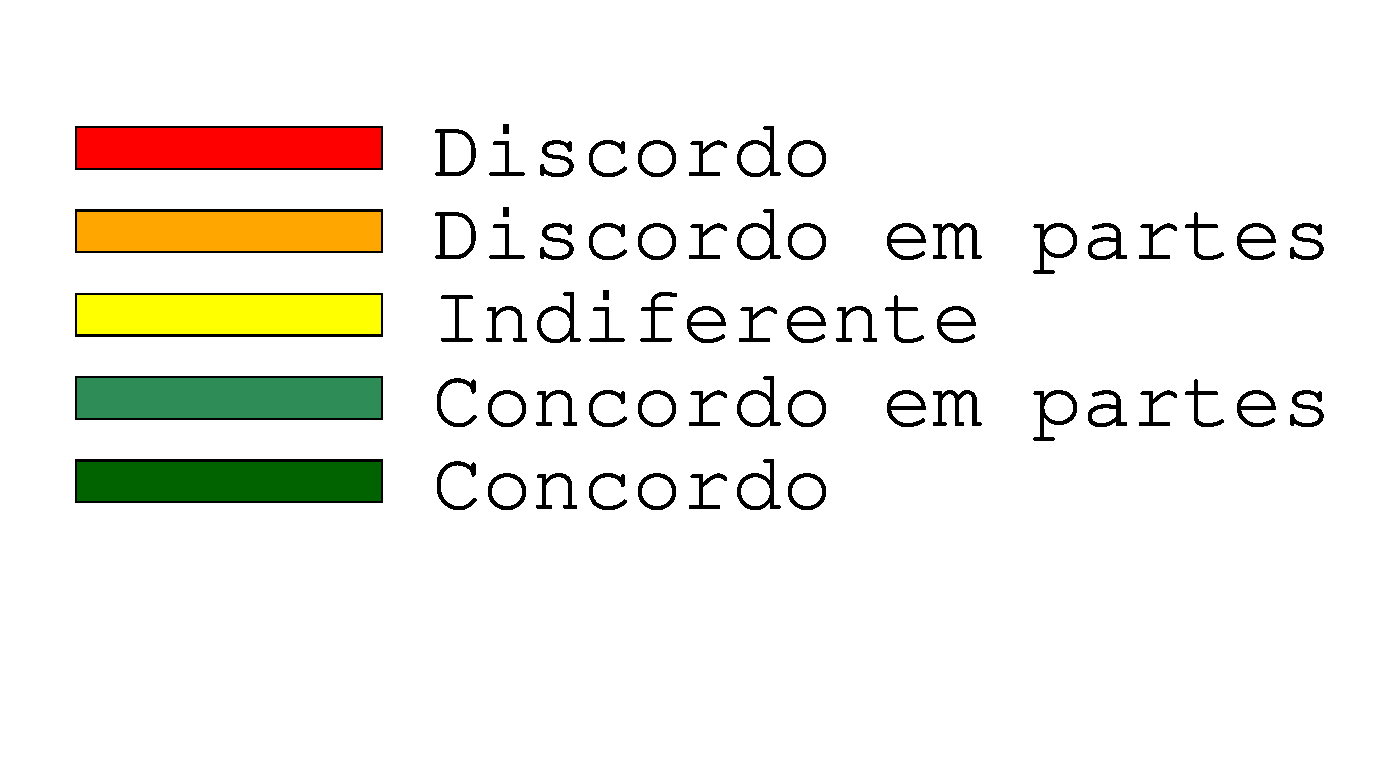
\includegraphics[scale=0.25,trim={50cm 25cm 0cm 0cm},clip]{figura-ref-graficos.eps}
\caption{Legenda para os gráficos em escala Likert} 
\label{figura-ref-graficos}
\end{figure}

Para cada replicação de problema foram construídos gráficos
dos resultados das respostas dos participantes para as afirmativas
de percepção e para a nota atribuída ao problema pelos
participantes em uma avaliação geral.


Nos gráficos sobre as percepções dos participantes
para afirmativas, a disposição nas barras
foi construída para facilitar a leitura por nível de favorabilidade.
A favorabilidade pode ser lida por porcentagem de satisfação,
em $y_1$ à esquerda, ou adicionalmente, por porcentagem de
insatisfação em $y_2$ à direta.
No caso de analisar os resultados em uma perspectiva conservadora ao máximo,
é possível considerar como favorável apenas a concordância
integral, isto é, o participante respondeu ``concordo'' para
a afirmação.
A consideração de concordância em parte como favorável,
isto é, também considerar favorável que
o participante respondeu ``concordo em partes'' para a afirmação,
apresenta um resultado menos conservador em relação ao caso anterior.
E assim por diante, com a consideração da resposta `indiferente'', que
representará o caso de favorabilidade onde não há de alguma forma de
discordância, etc.

Ao longo da discussão, ao mencionar textualmente uma afirmativa de
algum dos formulários, foi incluído entre parênteses a qual barra o texto
está se referindo, por exemplo, ``gosto da metodologia PBL (X)''.

Nos gráficos para os resultados das notas atribuídas pelo participante,
existem duas projeções, sendo uma projeção de barras com
a leitura em $y_1$ à esquerda e uma projeção em curva
em $y_2$ à direita.
Ambas as projeções utilizam $x$ na parte de baixo para as notas
inteiras atribuídas de $0$ a $10$.
Em $y_1$ a leitura tem o significado de quantas respostas, valor absoluto,
que foram atribuídas para uma determinada nota, ou seja,
o tamanho da barra.
No caso de $y_2$ o significado é do percentil igual ou superior
a um determinado valor, isto é,
qual a porcentagem da distribuição das barras que é igual ou superior
a uma determinada nota.

Para as discussões e conclusões apresentadas neste trabalho
sobre percepção foi considerada que uma afirmação obteve
resultado favorável ou positivo
se obteve $70\%$ de satisfação,
sendo favoráveis as percepções com algum nível de concordância,
isto é, o participante respondeu ``concordo''
ou ``concordo parcialmente''.

Nas seções a seguir que detalham os resultados de percepção sobre o problema, 
serão discutidos apenas os pontos principais observados,
positivos e negativos, em torno da favorabilidade para o
resultado positivo dentro dos critérios
definidos no parágrafo anterior.
A discordância integral nas afirmativas será destacada para que
os possíveis pontos de melhoria estejam mais explicitados em meio
aos resultados positivos.

A Tabela~\ref{tabela-ref-graficos2} apresenta
o significado das barras nos gráficos referentes às percepções
dos participantres para as afirmações mencionadas
na Seção~\ref{form-disciplinas} sobre a aplicação da disciplina,
para estudante \textit{concluinte},
e a Figura~\ref{figura-ref-graficos} apresenta a legenda (cor da barra)
nestes gráficos.

\begin{table}[ht]
\caption{Referências para os gráficos de percepção de estudante \textit{concluinte} sobre a disciplina}
\label{tabela-ref-graficos2}
\begin{tabular}{c|p{14.6cm}}
Legenda & Afirmativa respondida pelo participante \\
\hline
CA & \LikertCA\\
\hline
CB & \LikertCB\\
\hline
CC & \LikertCC\\
\hline
CD & \LikertCD\\
\hline
CE & \LikertCE\\
\hline
CF & \LikertCF\\
\hline
CG & \LikertCG\\
\hline
CH & \LikertCH\\
\hline
CI & \LikertCI\\
\hline
CJ & \LikertCJ\\
\hline
CK & \LikertCK\\
\hline
CL & \LikertCL\\
\hline
CM & \LikertCM\\
\hline
CN & \LikertCN\\
\end{tabular}
\end{table}


A Tabela~\ref{tabela-ref-graficos3} apresenta
o significado das barras nos gráficos referentes às percepções
dos participantres para as afirmações mencionadas
na Seção~\ref{form-disciplinas} sobre a aplicação da disciplina,
para estudante \textit{desistente},
e a Figura~\ref{figura-ref-graficos} apresenta a legenda (cor da barra)
nestes gráficos.

\begin{table}[h]
\caption{Referências para os gráficos de percepção de estudante \textit{desistente} sobre a disciplina}
\label{tabela-ref-graficos3}
\begin{tabular}{c|p{14.6cm}}
Legenda & Afirmativa respondida pelo participante \\
\hline
DA & \LikertDA\\
\hline
DB & \LikertDB\\
\hline
DC & \LikertDC\\
\hline
DD & \LikertDD\\
\hline
DE & \LikertDE\\
\hline
DF & \LikertDF\\
\hline
DG & \LikertDG\\
\hline
DG1 & \LikertDGa\\
\hline
DH & \LikertDH\\
\hline
DI & \LikertDI\\
\hline
DJ & \LikertDJ\\
\hline
DO & \LikertDO\\
\hline
DO1 & \LikertDOa\\
\end{tabular}
\end{table}


Para cada semestre de replicação, foram construídos gráficos
de resultados para as respostas dos participantes para as afirmativas
de percepção e para a nota atribuída para a disciplina pelos participantes
em uma avaliação geral.
%Para cada característica de participante, concluinte
%ou desistente, foram construídos quatro gráficos
%de resultados.
%Dois gráficos que exibem os resultados para as respostas
%dos participantes para as afirmativas de percepção,
%para os semestre 2016.1 e 2017.1, enquanto os outros dois gráficos
%exibem os resultados da nota geral atribuída pelos participantes.

Os artifícios utilizados para exibição dos gráficos e
discussão da percepção sobre a disciplina são os mesmos
utilizados nos gráficos e discussão da percepção sobre
o problema.
A disposição nas barras, a referência ao mencionar textualmente
uma afirmativa, valor absoluto e percentil nos gráfico da
nota geral etc.

\section{Semestre 2016.1}
\label{sec-sem-2016}
\resultadoTurma{2016.1}{26}{9}{6}{57,7}{11}{8}{3}

\subsection{Problema 1 -- \ProblemaA}
\perfilProblema{\ProblemaA}{1}{2016.1}{14}
\perfilParticipante{27,9}{20}{51}{35,7}{71,4}{entre o terceiro e o quinto semestre}{}
\figuraPercepcaoParticipante{s1p1}{1}{2016.1}

É possível destacar que para todas as questões a favorabilidade
foi superior aos $70\%$. A favorabilidade foi superior aos $90\%$
para 12 afirmações apresentadas.
Apenas 6 afirmações receberam ao menos uma discordância integral.

A afirmação sobre ideias alternativas no caminho do problema (B)
foi a que teve a maior percepção de concordância por partes dos
participantes.
Entendemos que este resultado é explicado pelo problema
ter apresentado os conceitos de músicas, de forma que
os participantes precisaram realizar relacionamentos entre
os conceitos deste tema com os conceitos de linguagens
formais, e que os participantes perceberam que a depender do
nível de abstração poderá existir um caminho diferente.


A necessidade de recorrer aos materiais de apoio (D),
existência de informações suficientes no texto (K) e
sobre o participante gostar da metodologia baseada
em problemas (X) foram as afirmações com
as menores favorabilidades.
Embora possa parecer existir alguma contradição
sobre os resultados das duas primeiras, vale
ressaltar que os dados referente
a contribuição da sessão tutorial (Q) obtiveram
alta favorabilidade.

\figuraPercepcaoParticipanteNotas{s1p1}{1}{2016.1}{80}{5,00}{7,29}{quase}

\subsection{Problema 2 -- \ProblemaB}
\perfilProblema{\ProblemaB}{2}{2016.1}{12}
\perfilParticipante{28,5}{20}{51}{25,0}{75,0}{entre o terceiro e o quinto semestre}{}
\figuraPercepcaoParticipante{s1p2}{2}{2016.1}

Para 5 afirmações, na percepção dos estudantes, a favorabilidade foi integral.
Em 15 afirmações a favorabilidade superou os $90\%$.
Em apenas uma das afirmações a favorabilidade ficou pouco abaixo dos $70\%$, onde
$66,7\%$ dos participante acreditam que o problema estimulou
o trabalho em grupo (M).
Apenas 5 afirmações receberam ao menos uma discordância integral.

A contribuição dos tutores para a evolução do problema (U) foi a
afirmação melhor avaliada pelos participantes, assim como as demais
afirmações referentes aos tutores (W) e (V) também foram bem avaliadas,
indicando que os participantes aprovaram a participação
dos tutores na condução deste problema.

Para a construção do produto deste problema, os participantes
precisaram se reunir em equipe além das sessões tutoriais, desta forma,
acreditamos que as dificuldades referentes a se reunir fora das sessões tutorias
para trabalhar em grupo (M) estão também representados neste resultado.
Também observamos uma justificativa para este resultado ao analisar a favorabilidade para
a afirmação referente a percepção dos participantes com relação a quantidade
apropriada de estudantes em cada grupo tutorial (S).

\figuraPercepcaoParticipanteNotas{s1p2}{2}{2016.1}{70}{6,00}{7,17}{mais de}

\subsection{Problema 3 -- \ProblemaC}
\perfilProblema{\ProblemaC}{3}{2016.1}{8}
\perfilParticipante{31,4}{20}{51}{28,6}{85,7}{até o quinto semestre}{ para cada três participantes}
\figuraPercepcaoParticipante{s1p3}{3}{2016.1}

Para 7 afirmações, na percepção dos estudantes, a favorabilidade foi integral.
Em três afirmações a favorabilidade ficou abaixo dos $70\%$, mas apenas 2
afirmações receberam ao menos uma discordância integral.

A contribuição das sessões tutorias para o processo
de resolução do problema (Q) obteve a melhor avaliação pelos
participantes.
Entendemos que essa afirmação é bem avaliada sempre que
os participantes conseguem perceber uma informação de
grande relevância para a solução durante a sessão
tutorial, neste caso, a ideia de como manipular a pilha
de forma a manter a proporção exigida pelo problema
surgiu durante uma sessão tutorial.

No que diz respeito a quantidade de pessoas em
cada grupo tutorial (S) ser a afirmação a obter a pior
avaliação a justificativa pode ser obtida quando
é observada em conjunto com a afirmação referente ao
trabalho em equipe (M) que também esteve entre
as piores avaliações para este problema, neste caso,
ambos resultados são explicados pela quantidade de
participantes nas sessões tutoriais.

\figuraPercepcaoParticipanteNotas{s1p3}{3}{2016.1}{90}{6,00}{7,50}{quase}

\subsection{Problema 4 -- \ProblemaD}
\perfilProblema{\ProblemaD}{4}{2016.1}{8}
\perfilParticipante{31,5}{20}{51}{25,0}{87,5}{até o quinto semestre}{}
\figuraPercepcaoParticipante{s1p4}{4}{2016.1}

Para 12 afirmações, na percepção dos estudantes, a favorabilidade foi integral.
Em todas as afirmações a favorabilidade ficou acima dos $70\%$.
Em 4 afirmações foi recebida ao menos uma discordância integral.

A máquina de Turing foi o principal objetivo de aprendizagem para o Problema 4
aplicado no semestre 2016.1, sendo que para os participantes a afirmação
melhor avaliada diz respeito a utilidade dos conhecimentos aprendidos para 
o profissional da área de Computação (I).
Este problema foi muito bem avaliado pelos participantes para todas
as afirmações, mas cabe destacar os resultados para as afirmações que
dizem respeito a necessidade de aprender novos conhecimentos (G) e
motivação dos participantes para resolver o problema (E).

\figuraPercepcaoParticipanteNotas{s1p4}{4}{2016.1}{90}{5,00}{7,50}{quase}

\subsection{Problema 5 -- \ProblemaE}
\perfilProblema{\ProblemaE}{5}{2016.1}{7}
\perfilParticipante{32,3}{20}{51}{28,6}{71,4}{até o quinto semestre}{}
\figuraPercepcaoParticipante{s1p5}{5}{2016.1}

Para 6 afirmações, na percepção dos estudantes, a favorabilidade foi integral.
Em apenas duas afirmações a favorabilidade ficou abaixo dos $70\%$.
Em 9 afirmações foi recebida ao menos uma discordância integral, desta forma,
indicando vários pontos de atenção para a abordagem deste problema
em outras situações.

Este também foi um problema em que os participantes se reuniram em grupo para
construir uma solução, assim, como no Problema 2 no semestre 2016.1, a
afirmação pior avaliada também foi referente ao trabalho em equipe (M) que
indicamos que o resultado também inclui as dificuldades em se reunir além
das sessões tutoriais.

Ideias alternativas (B), utilização de referências bibliográficas (C),
recorrer a materiais não indicados nas referências (D), motivação
para resolver o problema (E), o tempo para resolução (L), a quantidade de
pessoas no grupo da sessão tutorial (S), utilidade do problema para o
processo de ensino e aprendizagem (T), \textit{feedback} dos
tutores (W), além da afirmação sobre o trabalho em equipe (M)
mencionado no parágrafo anterior, foram as afirmações com ao menos
uma discondância integral.
O mais possível é que este resultados sejam justificados pela sobrecarga
adicional que os estudantes possuem no fim do semestre, momento em que
este problema foi aplicado.
Ainda assim, não se deve desconsiderar que estes são pontos
de atenção claros, mas que mesmo em outras metodologias, com pesquisa
semelhante, os resultados da sobrecarga estariam também explicitados.

\figuraPercepcaoParticipanteNotasA{s1p5}{5}{2016.1}{70}{}{7,00}{pouco mais de}

\section{Semestre 2017.1}
\label{sec-sem-2017}
\resultadoTurma{2017.1}{50}{x}{y}{z}{a}{14}{b}


\subsection{Problema 1 -- \ProblemaG}
\label{sec-2017-p1}
\perfilProblema{\ProblemaG}{1}{2017.1}{12}
\perfilParticipante{26,1}{19}{44}{18,2}{72,7}
{até o terceiro semestre}{ para cada seis participantes}
\figuraPercepcaoParticipante{s2p1}{1}{2017.1}

Para 7 afirmações apresentadas a favorabilidade ficou um pouco abaixo dos $70\%$, mas
para 10 afirmações foi superior aos $90\%$.
Em 11 afirmações foi recebida ao menos uma discordância integral.

Neste problema com o objetivo de aprendizagem foi Linguagens
Formais, sendo consenso de percepção dos participantes que
este problema apresenta um conhecimento útil para um profissional
da área de Computação (I).

É possível destacar o excelente resultado para a afirmação que diz respeito a
utilidade do problema no processo de ensino e aprendizagem (T).
A explicação para este resultado está no fato de que os estudantes
conseguiram realizar bem as correlações entre os conceitos
do código Morse, apresentado no problema, com os conceitos de
linguagens formais, que são os objetivos de aprendizagem para
este problema.

Em uma análise mais detalhada dos dados foi possível
detectar que a discordância integral está concentrada
em 3 participantes, onde apenas um destes apresentou
5 discordâncias integrais.
Estes números além de indicar pontos possíveis de
priorização, também podem indicar a necessidade
de um nivelamento maior dos estudantes para a aplicação
da metodologia.

\figuraPercepcaoParticipanteNotas{s2p1}{1}{2017.1}{90}{5,00}{8,25}{quase}

\subsection{Problema 2 -- \ProblemaB}
\perfilProblema{\ProblemaB}{2}{2017.1}{13}
\perfilParticipanteA{24,3}{19}{38}{8,3}{63,6}
{até o terceiro semestre}{ quatro para cada dez}
\figuraPercepcaoParticipante{s2p2}{2}{2017.1}

A favorabilidade ficou um pouco abaixo dos $70\%$ em 6 afirmações apresentadas,
sendo superior aos $80\%$ em 12 afirmações.
Em 14 afirmações foi recebida ao menos uma discordância integral.

Neste problema o objetivo de aprendizagem principal foi
Autômatos Finitos, sendo consenso de percepção dos participantes que
este problema apresenta um conhecimento útil para um profissional
da área de Computação (I) e que é necessário aprender novos
conhecimentos (G).

Apenas um dos participantes respondeu com discordância integral para
8 afirmações, assim, também se faz necessário considerar a
necessidade de nivelamento do grupo, como mencionado
na Seção~\ref{sec-2017-p1}.

Apesar de obter favorabilidade muito próxima aos $70\%$, a afirmação
sobre o participante gostar da metodologia PBL (X) teve como
destaque negativo receber a maior discordância integral nessa
replicação.

\figuraPercepcaoParticipanteNotas{s2p2}{2}{2017.1}{60}{5,00}{7,31}{pouco mais de}

\subsection{Problema 3 -- \ProblemaC}
\perfilProblema{\ProblemaC}{3}{2017.1}{11}
\perfilParticipanteA{25,1}{19}{38}{0}{63,6}
{até o terceiro semestre}{ quatro para cada dez}
\figuraPercepcaoParticipante{s2p3}{3}{2017.1}

A favorabilidade ficou um pouco abaixo dos $70\%$ em apenas uma afirmação,
sendo superior aos $80\%$ para 21 destas afirmações.
Em apenas 2 afirmações foi recebida ao menos uma discordância integral.

Para este caso a percepção dos participantes
sobre a relevância das sessões tutorias no processo
de resolução do problema (Q), assim como no semestre
anterior, obteve favorabilidade integral, com o destaque de
que para este semestre todas as respostas recebidas foram de
total concordância.

A afirmativa pior avaliada diz respeito a percepção dos participantes
sobre o \textit{feedback} dos tutores a cada sessão tutorial (W).
Para este caso, apesar do resultado ainda ser alto, ficou como
um ponto de atenção aos tutores.

A Figura~\ref{aval-s2p3} apresenta o gráfico da
avaliação do participantes para o Problema 3 aplicado no semestre 2017.1.

\begin{figure}[!htb]
\centering
\includegraphics[scale=0.18]{notas-s2p3.eps}
\caption{Avaliação dos participantes do semestre 2017.1 para o Problema 3}
\label{aval-s2p3}
\end{figure}

Assim como no semestre anterior, este problema foi muito bem avaliado
pelos participantes, assim, todas as notas atribuídas foram maiores
ou iguais $7,00$ e uma média de $8,18$.

Entre os problemas que foram replicados em ambos os semestres, este
notadamente é o que apresentou as melhores avaliações pelos participantes
em todos os critérios, evidenciando o potencial da metodologia em uma
disciplina teórica com a utilização de um problema do ``mundo real''.

\subsection{Problema 4 -- \ProblemaD}
\perfilProblema{\ProblemaD}{4}{2017.1}{10}
\perfilParticipanteB{25,7}{19}{38}{11,1}{88,9}
{até o terceiro semestre}{igual}
\figuraPercepcaoParticipante{s2p4}{4}{2017.1}

Para todas as afirmativas a percepção dos participantes obteve favorabilidade
superior aos $70\%$. Em 5 afirmações foi recebida ao menos uma discordância
integral.

O destaque positivo para este problema foi a favorabilidade em relação
a necessidade de recorrer a materiais fora da bibliografia básica (D).
Este é uma característica de estudo muito relevante no desenvolvimento
do estudante que passa a ver a necessidade de explorar fontes diversas
de informação para construir o seu conhecimento.

Como ponto de atenção, apesar de a favorabilidade ser igual aos $70\%$ para
a percepção do participante sobre a adequação do tempo disponível para desenvolver
a solução (L), houve uma quantidade relevante de discordância integral para esta afirmativa.

Este foi outro problema que foi bem avaliado em todos os critérios em ambos
os semestres.
\figuraPercepcaoParticipanteNotas{s2p4}{4}{2017.1}{80}{6,00}{7,31}{quase}

\subsection{Problema 5 -- \ProblemaE}
\perfilProblema{\ProblemaE}{5}{2017.1}{7}
\perfilParticipanteB{27,0}{20}{38}{20,0}{100,0}
{até o terceiro semestre}{semelhante}
\figuraPercepcaoParticipante{s2p5}{5}{2017.1}

Em 3 afirmações a favorabilidade ficou abaixo dos $70\%$ e 5 afirmações
receberam ao menos uma discordância integral.

Em contraste com o resultado que o mesmo problema teve com
os participantes do semestre 2016.1, onde foi a afirmação com a
pior favorabilidade, para os participantes neste semestre de
2017.1, a percepção de que o problema estimula o
trabalho em grupo (M) foi a afirmação melhor avaliada
para o Problema 5.
A diferença de resultado é justificada ao observar
a percepção dos participantes com relação a quantidade
apropriada de estudantes em cada grupo tutorial (S).

A afirmação com a menor favorabilidade diz respeito
a percepção de cumprimento dos objetivos de aprendizagem
pelo participante (F).
Neste ponto cabe destacar que ao apresentar um resultado
negativo para esta afirmação, uma vez que com outros
problemas dentro do mesmo grupo tiveram favorabilidade
melhores, se pode questionar o problema e não
a metodologia.
Também não se pode deixar de considerar o nível de abstração
mais elevado para o entendimento dos conceitos deste
problema em relação aos demais.

\figuraPercepcaoParticipanteNotas{s2p5}{5}{2017.1}{70}{5,00}{7,43}{pouco mais de}


\subsection{Percepção dos concluintes}
\QtdParticipantes{2016.1}{11}{1}{6}
\perfilParticipante{28,8}{20}{49}{50,0}{83,3}{até o quarto semestre}{}
\figuraPercepcaoParticipanteDisciplina{concluintes-2016}{concluintes}{2016.1}
\AprovacaoDisciplina{83,3}{}{aprovação da metodologia para a}%
{a metodologia}{CA}{2016.1}{concluintes}
\AprovacaoDisciplinaC{66,7}{83,3}
\AprovacaoDisciplinaD{100,0}{ter várias avaliações}{CD}
\AprovacaoDisciplinaE{83,3}{avaliações em equipe}{CE}
\AprovacaoDisciplina{100,0}{}{avaliação dos tutores na}%
{os tutores}{CF}{}{}
\AprovacaoDisciplinaG{2016.1}{4}{6}{75,0}{CG}
\AprovacaoDisciplinaA{100,0}{entenderam a metodologia PBL}{CH}
\AprovacaoDisciplinaF{16,7}{é um problema falar em público}{CI}{não}
\AprovacaoDisciplinaB{100,0}{experimentar outras abordagens além das aulas tradicionais}{CJ}{}{}
\AprovacaoDisciplinaA{83,3}{a metodologia PBL ajudou nas avaliações escritas}{CK}
\AprovacaoDisciplinaA{83,3}{a metodologia PBL ajudou a entender melhor os conceitos}{CL}
\AprovacaoDisciplinaF{66,7}{que há um balanceamento satisfatório na distribuição de carga
horária entre sessões tutoriais e aulas expositivas}{CM}{}
\AprovacaoDisciplinaB{83,3}{experimentar outras disciplinas com PBL}{CN}{}{0,0}

\figuraPercepcaoParticipanteDisciplinaNotas{2016-concluintes}{concluintes}{2016.1}{100,0}{}{7,83}{}

\QtdParticipantes{2017.1}{x}{1}{12}
\perfilParticipanteB{22,75}{20}{28}{16,7}{58,3}{até o terceiro semestre}{semelhante}
\figuraPercepcaoParticipanteDisciplina{concluintes-2017}{concluintes}{2017.1}
\AprovacaoDisciplina{100,0}{}{aprovação da metodologia para a}%
{a metodologia}{CA}{2017.1}{concluintes}
\AprovacaoDisciplinaC{75,0}{66,7}
\AprovacaoDisciplinaE{75,0}{ter várias avaliações}{CD}
\AprovacaoDisciplinaE{83,3}{avaliações em equipe}{CE}
\AprovacaoDisciplina{100,0}{}{avaliação dos tutores na}%
{os tutores}{CF}{}{}
\AprovacaoDisciplinaG{2017.1}{9}{12}{55,6}{CG}
\AprovacaoDisciplinaA{75,0}{entenderam a metodologia PBL}{CH}
\AprovacaoDisciplinaF{25,0}{é um problema falar em público}{CI}{não}
\AprovacaoDisciplinaB{91,7}{experimentar outras abordagens além das aulas tradicionais}{CJ}%
{apenas}{8,3}
\AprovacaoDisciplinaA{66,7}{a metodologia PBL ajudou nas avaliações escritas}{CK}
\AprovacaoDisciplinaA{75,0}{a metodologia PBL ajudou a entender melhor os conceitos}{CL}
\AprovacaoDisciplinaF{66,7}{que há um balanceamento satisfatório na distribuição de carga
horária entre sessões tutoriais e aulas expositivas}{CM}{}
\AprovacaoDisciplinaB{66,7}{experimentar outras disciplinas com PBL}{CN}{apenas}{8,3}

\figuraPercepcaoParticipanteDisciplinaNotas{2017-concluintes}{concluintes}{2017.1}{80}{5,00}{7,83}{mais de}

\subsection{Percepção dos desistentes}
\QtdParticipantes{2016.1}{15}{0}{3}
\perfilParticipanteC{24,0}{23}{25}{66,7}{100,0}{até o sétimo semestre}{}
\figuraPercepcaoParticipanteDisciplina{desistentes-2016}{desistentes}{2016.1}
\AprovacaoDisciplina{0,0}{desistentes}{aprovação da abordagem para a}%
{a abordagem}{DA}{}{}
Nenhum dos participantes apresentou como motivo para a desistência a
oposição em ter a presença como critério de avaliação (DB) e
em ter várias avaliações (DD), mas existe oposição por $33,3\%$
em ter a participação nas aulas como critério de avaliação (DC) e em ter
avaliações em equipe (DE).
Os tutores não foram motivadores da desistência (DF) para nenhum
dos desistentes.
Dificuldade de conciliar a disciplina com
o trabalho profissional (DG) e questões pessoais (DG1)
foram os motivos mais apontados para desistência,
com $66,7\%$.
\AprovacaoDisciplinaA{66,7}{entenderam a abordagem \ac{PBL}}{DH}
\AprovacaoDisciplinaH{33,7}{é um problema falar em público}{DI}{não}
\AprovacaoDisciplinaB{66,7}{experimentar outras abordagens além das aulas tradicionais}{DJ}{}{0,0}
Apesar de apenas $33,3\%$ dos participantes ter respondido ter interesse
em cursar a disciplina com abordagem \ac{PBL} (DO1) em outra oportunidade,
não existiu manifestação contrária.
Para $66,7\%$ a carga horária de aulas expositivas deveria ser maior (DO).

\figuraPercepcaoParticipanteDisciplinaNotasA{2016-desistentes}{desistentes}{2016.1}{30}
{5,00}{5,67}{apenas pouco mais de}

\QtdParticipantes{2017.1}{18}{0}{1}
\perfilParticipanteD{masculino}{23}{primeiro}{}{}
\figuraPercepcaoParticipanteDisciplina{desistentes-2017}{desistentes}{2017.1}
O participante apresentou concordância apenas para a desistência ter sido motivada
por não conseguir conciliar a disciplina com o trabalho profissional
dele (DG) e também por outras questões pessoais (DG1).
O participante considera que conseguiu entender a abordagem \ac{PBL} (DH),
que tem interesse em cursar a disciplina em outra oportunidade com
a abordagem \ac{PBL} (DO1), com mais carga horária de aula expositivas (DO) e
que gostaria de experimentar outras abordagens de ensino (DJ).
Não menciona que falar em público seja um problema (DI).

\SemFiguraPercepcaoParticipanteDisciplinaNotas{desistente}{2017.1}

O participante desistente atribuiu nota $9,00$ como avaliação da
disciplina.
A nota atribuída reforça que como os dados de percepção demonstra,
o participante desistiu da disciplina por motivos externos, no caso,
não conseguiu conciliar o trabalho profissional que exerce com
a disciplina (DG).


\section{Avaliações dos objetivos específicos}
\label{sec-avaliacao-hipoteses}
Para avaliação dos objetivos específicos as quais este estudo se propõe,
utilizamos os resultados apresentados neste capítulo.

Para a avaliação dos objetivos específicos deste estudo, uma vez que a
metodologia utilizada exige que alguns critérios sejam
arbitrados, preferimos ser bastante conservadores
na definição dos parâmetros arbitrados.
No caso de um objetivo com apenas uma afirmação, consideramos
como avaliação positiva se a afirmação recebe
resultado positivo dentro dos critérios mencionados na
Seção~\ref{sec-ref-graficos}, ou seja, $70\%$ de favorabilidade,
sendo favoráveis as respostas de concordância.
No caso de mais de uma afirmativa, consideramos
como avaliação positiva em caso de resultado positivo para todas
as afirmativas, dentro dos mesmos critérios de favorabilidade.

Destacamos que a avaliação dos objetivos específicos foi realizada para
cada replicação de problema, ou seja, é possível concluir com
uma avaliação positiva em uma replicação de problema, enquanto pode
não ser possível concluir com uma avaliação positiva em outra replicação
de problema.

% OE1
\AvaliacaoObjetivo{\oeatexto}{oe1ref}{oe}{``\LikertPQ'' (Q)}{}{}{}{}{}

\AprovacaoObjetivo{}{}{todas}{0}{}
\ObjetivoFavorabilidadeDestaque{}{\ProblemaC}{2017.1}{100,0}{}{}
\ObjetivoFavorabilidadeDestaqueContinuidade{2016.1}{100,0}{}
\ObjetivoFavorabilidadeDestaqueDiferencas{2016.1}{25,0}{2017.1}{100,0}
\ObjetivoFavorabilidadeDestaqueOutra{}{\ProblemaD}{2016.1}{100}{}
\ObjetivoFavorabilidadeDestaqueContinuidade{2017.1}{90,0}{}
\AprovacaoObjetivoResultado{}{}{}{}{}{}{}{}{}

% OE2
\AvaliacaoObjetivo{\oebtexto}{oe2ref}{oe}{``\LikertPM'' (M)}{}{}{}{}{}

\AprovacaoObjetivo{}{não}{3}{0}{}
\AprovacaoObjetivoResultado{não}{\ProblemaB}{\ProblemaC}{\ProblemaE}{2016.1}{}{}{}{}
Em nosso trabalho \cite{gavaza2017}, que utilizamos apenas dados do
semestre 2016.1, apesar de não termos definidos parâmetros
de avaliação, percebemos que a percepção dos estudantes com relação
a motivação para o trabalho em equipe também não recebeu as melhores
avaliações.
No semestre 2016.1, como descrito na Seção ~\ref{sec-exp-2016}, foi utilizado
apenas um quadro branco, assim foi formado apenas um grupo com todos
os estudantes.
Para o semestre 2017.1, como descrito na Seção ~\ref{sec-exp-2017}, foram
utilizados quadros adicionais e foram formados grupos menores,
de até dez participantes cada.
\AprovacaoObjetivo{}{}{todas}{0}{2017.1}
\ObjetivoFavorabilidadeDestaque{}{\ProblemaE}{}{100,0}{85,7}{}
% escrever sobre a redução no grupo tutorial e qual a conclusão

% OE3
\AvaliacaoObjetivo{\oectexto}{oe3ref}{oe}{``\LikertPT'' (T)}{}{}{}{}{}

\AprovacaoObjetivo{}{}{todas}{0}{}
\ObjetivoFavorabilidadeDestaque{}{\ProblemaC}{2016.1}{100,0}{50,0}{\ProblemaD}
\ObjetivoFavorabilidadeDestaqueContinuidade{2017.1}{90,9}{80,0}
\ObjetivoFavorabilidadeDestaqueOutra{}{\ProblemaG}{2017.1}{91,7}{91,7}
\ProblemaSemReplica{2016.1}{}
\AprovacaoObjetivoResultado{}{}{}{}{}{}{}{}{}

% OE4
\AvaliacaoObjetivo{\oedtexto}{oe4ref}{}{``\LikertPC'' (C)}{``\LikertPD'' (D)}
{``\LikertPG'' (G)}{``\LikertPK'' (K)}{``\LikertPO'' (O)}{``\LikertPP'' (P)}

\ObjetivoNaoAtende{\ProblemaG}{2017.1}{(C)}{(D)}{(O)}{}{}{}{}
\ProblemaSemReplica{2016.1}{\ProblemaG}
\ObjetivoNaoAtende{\ProblemaB}{2017.1}{(C)}{(D)}{(P)}{}{}{}{}
\ObjetivoAtende{\ProblemaB}{2016.1}{p}
\AprovacaoObjetivo{}{não}{2}{1}{}
\AprovacaoObjetivoResultado{não}{\ProblemaG}{\ProblemaB}{}{2017.1}{}{}{}{}

% OE5
\AvaliacaoObjetivo{\oeetexto}{oe5ref}{oe}{``\LikertPU'' (U)}{``\LikertPV'' (V)}
{``\LikertPW'' (W)}{}{}{}

\ObjetivoNaoAtende{\ProblemaG}{2017.1}{(W)}{}{}{}{}{}{}
\ProblemaSemReplica{2016.1}{\ProblemaG}
\ObjetivoNaoAtende{\ProblemaB}{2017.1}{(W)}{}{}{}{}{}{}
\ObjetivoAtende{\ProblemaB}{2016.1}{p}
\ObjetivoNaoAtende{\ProblemaC}{2017.1}{(W)}{}{}{}{}{}{}
\ObjetivoAtende{\ProblemaC}{2016.1}{p}
\ObjetivoNaoAtende{\ProblemaE}{2017.1}{(W)}{}{}{}{}{}{}
\ObjetivoAtende{\ProblemaE}{2016.1}{p}
A favorabilidade não foi atingida em 4 das 5 replicações no
semestre 2017.1.

% OE6
\AvaliacaoObjetivo{\oeftexto}{oe6ref}{oe}{``\LikertPI'' (I)}{}{}{}{}{}

\AprovacaoObjetivo{}{}{todas}{0}{}
\ObjetivoFavorabilidadeDestaque{}{\ProblemaC}{2017.1}{100,0}{90,9}{}
\ObjetivoFavorabilidadeDestaqueContinuidade{2016.1}{75,0}{}
\MaisDestaque{4}{5}{2017.1}{85,8}{\ProblemaE}
\AprovacaoObjetivoResultado{}{}{}{}{}{}{}{}{}

% OE7
\AvaliacaoObjetivo{\oegtexto}{oe7ref}{oe}{``\LikertPA'' (A)}{``\LikertPB'' (B)}{}{}{}{}

\ObjetivoNaoAtende{\ProblemaE}{2016.1}{(B)}{}{}{}{}{}{}
\ObjetivoAtende{\ProblemaE}{2017.1}{p}
\ObjetivoNaoAtende{\ProblemaG}{2017.1}{(B)}{}{}{}{}{}{}
\ProblemaSemReplica{2017.1}{\ProblemaG}
\AprovacaoObjetivoResultado{não}{\ProblemaE}{}{}{2016.1}{\ProblemaG}{}{}{2017.1}

\subsection{Síntese dos objetivos específicos}
A Tabela~\ref{tabela-ref-objetivos} apresenta
uma síntese das avaliações dos objetivos específicos.
\begin{table}[h]
\caption{Síntese de avaliação dos objetivos específicos}
\label{tabela-ref-objetivos}
\begin{tabular}{p{6.5cm}|c|c|c|c|c|c|c|c|c|c}

\hfil\multirow{2}{*}{Objetivo}\hfill & \multicolumn{5}{c|}{2016.1} &
\multicolumn{5}{c}{2017.1} \\

\cline{2-11}
	 & PA & PB & PC & PD & PE &
           PG & PB & PC & PD & PE \\
\hline
% HE1
\allOK{\oeatexto}
\hline
% HE2
\noAllOKA{\oebtexto}{1}{0}{0}{1}{0}
\noAllOKB{1}{1}{1}{1}{1}
\hline
% HE3
\allOK{\oectexto}
\hline
% HE4
\noAllOKA{\oedtexto}{1}{1}{1}{1}{1}
\noAllOKB{0}{0}{1}{1}{1}
\hline
% HE5
\noAllOKA{\oeetexto}{1}{1}{1}{1}{1}
\noAllOKB{0}{0}{0}{1}{0}
\hline
% HE6
\allOK{\oeftexto}
\hline
% HE7
\noAllOKA{\oegtexto}{1}{1}{1}{1}{0}
\noAllOKB{0}{1}{1}{1}{1}
\hline
\end{tabular}
\legendaTabelaSintese
\end{table}


É possível perceber que apenas o problema ``\ProblemaD'' obteve
avaliação positiva para todos os objetivos específicos em duas
replicações, conforme os critérios definidos, e que o
problema ``\ProblemaA'' obteve avaliação positiva para todos as
objetivos específicos na única replicação, conforme os
critérios definidos.

Existem dois principais resultados negativos facilmente
perceptíveis na síntese de avaliação dos objetivos
específicos.
O resultado para o objetivo específico em relação ao trabalho em equipe
para as replicações no semestre 2016.1 e para o objetivo
específico em relação contribuição positiva dos tutores nas
replicações do semestre 2017.1.
Os dois principais resultados negativos são justificáveis.

No caso do objetivo específico em relação ao trabalho em equipe
para as replicações no semestre 2016.1 o tamanho
do grupo tutorial é o principal argumento
para este resultado.

Entendemos que a divisão de grupos tutoriais menores
nas replicações do semestre 20171.1 contribuiu
positivamente para o trabalho em equipe dos
estudantes e consequentemente para a percepção destes
sobre este trabalho, assim, sugerimos que os
grupos tutoriais devem possuir entre cinco e dez estudantes,
como em nossa replicação do semestre 2017.1, para aumentar
as possibilidades dos resultados estarem dentro de critérios
semelhantes aos nossos.

No caso do objetivo específico em relação contribuição positiva
dos tutores nas replicações do semestre 2017.1 a quantidade de
tutores para o total de estudantes na turma é a justificativa.

Como não foi adotada nenhuma ação com relação ao aumento da
quantidade total de estudantes em relação ao semestre 2016.1,
de 26 para 50, quase o dobro, entendemos que os tutores não
puderam se aproximar mais efetivamente dos estudantes
nas replicações do semestre 2017.1.
Nossa experiência sugere que o ideal é disponibilizar um
tutor para facilitar a sessão tutorial para entre dez e
quinze estudantes.

Os objetivos específicos em relação à percepção dos estudantes sobre
a metodologia estimular a autoaprendizagem e sobre percepção de
conexões entre o conhecimento e o problema entendemos ser
resultados pontuais, que podem ser melhorados com adequações nos problemas
onde os resultados não foram positivos, uma vez que na maioria das replicações
os objetivos específicos em questão foram avaliados positivamente
dentro dos critérios definidos.


\newcommand{\contribuicoesQualitativas}[7]{%
{\ifthenelse{\equal{#5}{}}{O problema ``#1'' foi
replicado apenas no semestre #2 e}{
Na replicação do problema ``#1'' no semestre #2}}
foram recebidas contribuições discursivas%
{\ifthenelse{\equal{#3}{zero}}{}{ de #3
participante{\ifthenelse{\equal{#3}{um}}{}{s}}
sobre o problema{\ifthenelse{\equal{#4}{zero}}{}{ e}}}}%
{\ifthenelse{\equal{#4}{zero}}{}{ de #4
participante{\ifthenelse{\equal{#4}{um}}{}{s}}
sobre a metodologia PBL}}.%
{\ifthenelse{\equal{#5}{}}{}{
No semestre #5
{\ifthenelse{\equal{#6}{zero}}{{\ifthenelse{\equal{#7}{zero}}{não }{}}{}}{}}%
foram recebidas contribuições discursivas%
{\ifthenelse{\equal{#6}{zero}}{}{ de #6
participante{\ifthenelse{\equal{#6}{um}}{}{s}}
sobre o problema{\ifthenelse{\equal{#7}{zero}}{}{ e}}}}%
{\ifthenelse{\equal{#7}{zero}}{}{ de #7
participante{\ifthenelse{\equal{#7}{um}}{}{s}}
sobre a metodologia PBL}}.}}}

\newcommand{\contribuicoesQualitativasDisciplina}[5]{%
Entre os #1 estudantes #2 do semestre #3
{\ifthenelse{\equal{#4}{zero}}{{\ifthenelse{\equal{#5}{zero}}{não }{}}{}}{}}%
foram recebidas contribuições discursivas%
{\ifthenelse{\equal{#4}{zero}}{}{ de #4
participante{\ifthenelse{\equal{#4}{um}}{}{s}}
sobre a metodologia PBL{\ifthenelse{\equal{#5}{zero}}{}{ e}}}}%
{\ifthenelse{\equal{#4}{zero}}{}{ de #5
participante{\ifthenelse{\equal{#5}{um}}{}{s}}
sobre a disciplina}}.%
}

\section{Respostas discursivas}
\label{sec-sem-quali}

\subsection{\ProblemaA}
\contribuicoesQualitativas{\ProblemaA}{2016.1}{dois}{quatro}{}{}{}

Em relação ao problema ambos os participantes mencionam a complexidade.
Um participante diz que há dependência com os conceitos de música
e outro acredita que a complexidade está relacionada com este ser
o primeiro problema ao qual foram submetidos.

A metodologia foi avaliada positivamente, sendo
``interessante'', ``útil'', ``colaborativa'' e ``soluções rápidas''
as qualidades mais mencionadas.
Foi destacada também que a metodologia precisa de
aprimoramentos.

\subsection{\ProblemaB}
\contribuicoesQualitativas{\ProblemaB}{2016.1}{dois}{dois}{2017.1}{seis}{cinco}

Para este problema os participantes mencionaram a não especificação clara
do problema, sobretudo os participantes da replicação do semestre 2016.1.
Apesar de os participantes terem recebido
uma explicação sobre a metodologia e terem participado
do problema anterior com a metodologia PBL, é necessário considerarmos
que os participantes estão envolvidos em um curso tradicional
em que as atividades que executam nas outras disciplinas são normalmente
especificações, ao contrário do que é recomendado nos princípios citados
em \cite{dolmans1997seven} e que foram utilizados para
a construção deste problema.

Ainda sobre o problema, no caso da replicação do semestre 2017.1 a dificuldade
do problema é o assunto mais mencionado.
Embora exista divergência entre os participantes
sobre o acréscimo de dificuldade, a maioria menciona que este
problema é mais difícil que o anterior, no caso, ``\ProblemaG''.

Com relação a metodologia, os participantes da replicação do semestre 2016.1
mencionam a necessidade de mais retorno por parte dos tutores,
embora as avaliações referentes ao tutores tenham sido
os melhores avaliados quantitativamente, como destacamos
na Seção~\ref{sec-sem-2016} na apresentação dos resultados
da replicação deste problema.

Os participantes na replicação deste problema no semestre 2017.1
apresentaram algumas avaliações positivas para a metodologia
e alguns pontos de atenção no que diz respeito ao
comportamento necessário dos estudantes para o bom
andamento da metodologia.
As palavras ``desperta'', ``enriquecedor'', ``bom'' e ``\textit{insights}''
foram mencionadas positivamente em relação a metodologia e ``perdidos''
foi a palavra mencionada negativamente em relação a metodologia.
Foi mencionado que das reuniões alguns estudantes não conseguem
extrair as informações necessárias e que faltou aula teórica
de como fazer o autômato antes da aplicação do problema.

O compromisso dos estudantes é necessário para
o andamento de uma disciplina, independente de qual seja
o método utilizado.
No caso do PBL, as interações entre os envolvidos no processo
se fazem extremamente necessárias, nesse contexto,
foi citado por três participantes na replicação do semestre 2017.1 as dificuldades
com relação ao trabalho em equipe.

\subsection{\ProblemaC}
\contribuicoesQualitativas{\ProblemaC}{2016.1}{um}{um}{2017.1}{três}{dois}

Na replicação deste problema no semestre 2016.1
foi destacado o equilíbrio entre tempo e a dificuldade
que também é observado nos resultados quantitativos
na favorabilidade da afirmativa ``\LikertPL'' (L)
e mencionado uma maior participação
dos estudantes nesta replicação.

No caso da replicação no semestre 2017.1 a dificuldade
do problema é o assunto mais mencionado, onde o problema foi
qualificado com um dificuldade entre média e difícil.
Novamente apontado sobre o texto, acreditamos que o
envolvimento dos participantes em um curso
tradicional pode criar expectativas de que o texto
seja mais ``especificação''.

Sobre a metodologia PBL, na replicação do semestre 2017.1,
é mencionado a vontade em participar e o desafio trazido
pelo problema.
Também foi mencionado que outros estudantes não
demonstravam interesse e que isto de certa forma
contamina os estudantes interessados.

\subsection{\ProblemaD}
\contribuicoesQualitativas{\ProblemaD}{2016.1}{um}{zero}{2017.1}{três}{um}

Na replicação do semestre 2016.1, sobre o problema, foi mencionado
sobre a necessidade de construção mais simples nas aulas
expositivas para melhor entendimento do problema.
Também foi mencionado sobre as inúmeras possibilidades, em consonância
com os resultados qualitativos onde essa característica foi
percebida, em algum nível, por todos os participantes.

Para a replicação do problema no semestre 2017.1, foi mencionado
que este problema trata de um assunto real, assim como
os dados quantitativos, que podem ser observados
na afirmativa ``\LikertPH'' (H).
Também foi citado que a redução na quantidade de membros no grupo
tutorial, ocasionada pela ausência de estudantes, contribuiu
positivamente para as discussões.

Percebemos que alguns estudantes possuem um perfil mais passivo
de aprendizagem ou possuem outras obrigações que os impedem
de se dedicar em buscar conhecimento, nesse contexto,
um dos participantes, na replicação do problema no
semestre 2017.1, menciona a ausência de conhecimento
sobre o assunto como barreira para a aprendizagem.
Este problema foi construído seguindo
os princípios citados em \cite{dolmans1997seven},
portanto, considerando os conhecimentos prévios
dos estudantes, mas como foi considerado um perfil
genérico para estes, uma vez que não foi
traçado previamente os seus perfis, alguns estudantes
podem não ser exatamente contemplados.
A qualidade da metodologia PBL em estimular os estudantes
em buscar o conhecimento, como mencionado no trabalho
\cite{savery2015overview} é mais efetivo quando
existe essa aderência de perfil com o problema.
O resultado quantitativo, referente a motivação dos
participantes (E), é excelente para esta
replicação, assim, em análise conjunta com o
resultado qualitativo entendemos que o perfil
do participante em questão pode não ter sido
atingido pelo problema.

\subsection{\ProblemaE}
\contribuicoesQualitativas{\ProblemaE}{2016.1}{um}{um}{2017.1}{um}{um}

A dificuldade do problema foi mencionada em ambas as replicações, mas
também foi mencionado como interessante.
Com relação a disciplina, foi mencionado, por participante da
replicação do semestre 2016.1, que o problema deveria ser
mais extenso no conteúdo.
No caso de uma disciplina de Teoria da Computação, entendemos
que a construção de um problema com mais conceitos se
torna ainda mais complexa, em todos os sentidos, sobretudo
para conciliar as recomendações
no trabalho \cite{dolmans1997seven}.

\subsection{\ProblemaF}
\contribuicoesQualitativas{\ProblemaF}{2017.1}{dois}{dois}{2016.1}{zero}{zero}

Para este problema foi mencionada a dificuldade e a falta de estímulos
para resolver por ser um assunto mais matemático.
Os conceitos deste problema exigem um nível de abstração bem elevado
dos estudantes, e por maiores que sejam os esforços na construção
do problema não é simples construir um problema capaz de cumprir com
os objetivos de aprendizagem e que ``escondam'' as dificuldades
em meio ao problema.

No que diz respeito a disciplina, é destacado que a dificuldade
em sentir que possui uma resposta é um desmotivante.
Embora para este problema não tenha sido realizada uma replicação
completa da metodologia PBL, um participante mencionou que não
conseguiu se adaptar, neste caso, entendemos que possa estar
comentando também em relação a outros problemas.

\subsection{\ProblemaG}
\contribuicoesQualitativas{\ProblemaG}{2017.1}{dois}{dois}{}{}{}

Foi mencionado sobre o problema ser extenso e
apresentar uma situação diferente das que as pessoas fariam em caso
real.
O resultado quantitativo em relação ao tempo (L)
foi muito bem avaliado nesta replicação, então, entendemos que
para este caso pode ser uma percepção isolada.
No caso da situação apresentar uma situação real (H), o resultado
quantitativo é apenas razoável, o que está de acordo
com o que foi mencionado pelo participante, assim, para utilizar
este problema em outras replicações é interessante realizar adequações
da situação mencionada.

\subsection{Concluintes}
\contribuicoesQualitativasDisciplina{11}{concluintes}{2016.1}{dois}{dois}
\contribuicoesQualitativasDisciplina{}{concluintes}{2017.1}{três}{três}

Os comentários em relação a metodologia PBL foram na maioria elogiosos.
Foi mencionado que a metodologia ajuda no processo de aprendizagem da
disciplina, além de interessante e motivadora.

A aprendizagem mais profunda dos conteúdos e a necessidade de mais
esforço por parte dos estudantes também foram destacadas.
Acreditamos que nesse contexto, o objetivo de fazer com que
os estudantes assumam também a responsabilidade pela a
sua aprendizagem fica explicitada.
Apesar disto, verificamos que algumas afirmativas relacionadas
com estímulos para desenvolvimento de habilidades para autoaprendizagem
não foram das melhores avaliadas em todas as replicações,
como por exemplo, buscar outras referências de estudo (D),
estudar individualmente fora das sessões PBL (O) e buscar
conhecimento por motivação (P), na replicação dos
problemas ``\ProblemaG'' e ``\ProblemaB'' no semestre 2017.1.

Foi mencionado que alguns estudantes durantes as discussões
não participavam e que isto dificultava o andamento da sessão.
De fato, como mencionado nos
trabalhos \cite{savery2015overview} e \cite{albanese2010problem}
e baseados nas percepções durante as replicações, a eficiência da metodologia
também depende da colaboração entre os participantes.

Não está claro em qual contexto o estudante menciona como útil
para a metodologia PBL a criação de máquinas, uma vez que
foi percebido, em praticamente todas as replicações, que
existiram tentativas de criação das máquinas por partes
dos estudantes.
Acreditamos que alguns estudantes, por estarem em um curso
tradicional, podem de certa forma estarem bastante conectados
à imagem do professor tradicional como um repositório de
respostas.
Na metodologia PBL, o professor, no papel de tutor, é o facilitador
do processo, como mencionado em diversos trabalhos, como
\cite{hmelo2004problem} e \cite{savery2015overview}.
Em nossas percepções durante as replicações, percebemos que
parece ser a melhor estratégia para manter a discussão, ter um
espaço para a manifestações com o máximo de liberdade possível,
ainda que inicialmente possa parecer que a intervenção
de alguns estudante não vá contribuir para
a discussão.
O tutor deve intervir, sem contrapor, dentro das possibilidades,
apenas se percebe que a maioria dos estudantes estão se afastando
dos objetivos de aprendizagem.

Um dos participantes menciona que entende não ter se adequado
a metodologia PBL e este seria o motivo da reprovação por conceito,
apesar de ter destacado que a metodologia é ``interessante'' e ``inteligente''.
A nossa percepção, obtida na execução deste trabalho, é que a replicação
da metodologia PBL pode ser beneficiada com um mapeamento menos genérico
do perfil dos participantes, principalmente em cursos em que a maioria
das disciplinas utiliza uma abordagem tradicional para aprendizagem, que
é a situação da instituição de ensino onde replicamos este trabalho.

\subsection{Desistentes}
\contribuicoesQualitativasDisciplina{15}{desistentes}{2016.1}{um}{um}
\contribuicoesQualitativasDisciplina{x}{desistentes}{2017.1}{zero}{zero}


\section{Discussão das hipóteses}

% HG1
\AvaliacaoHipotese{\hatexto}{h1ref}{}{``\LikertPX'' (X)}{}{}{}{}{}

\AprovacaoObjetivo{}{não}{3}{0}{}
\AprovacaoObjetivoResultado{não}{\ProblemaC}{}{}{2016.1}{\ProblemaB}{\ProblemaE}{}{2017.1}
\ObjetivoFavorabilidadeDestaque{}{\ProblemaD}{2016.1}{87,5}{}{}
\ObjetivoFavorabilidadeDestaqueContinuidade{2017.1}{70,0}{}

% HG2
\AvaliacaoObjetivo{\hbtexto}{h2ref}{hg}{``\LikertPF'' (F)}{}{}{}{}{}

\AprovacaoObjetivo{}{não}{1}{0}{}
\AprovacaoObjetivoResultado{não}{\ProblemaE}{}{}{2017.1}{}{}{}{}
\ObjetivoFavorabilidadeDestaque{}{\ProblemaD}{2016.1}{100,0}{37,5}{}
\ObjetivoFavorabilidadeDestaqueContinuidade{2017.1}{70,0}{}

% HG3
\AvaliacaoObjetivo{\hctexto}{h3ref}{hg}{``\LikertPE'' (E)}{}{}{}{}{}

\AprovacaoObjetivo{}{}{todas}{0}{}
\ObjetivoFavorabilidadeDestaque{}{\ProblemaA}{2016.1}{92,9}{42,9}{}
\ProblemaSemReplica{2017.1}{\ProblemaA}
\ObjetivoFavorabilidadeDestaqueOutra{}{\ProblemaG}{2017.1}{91,7}{25,0}
\ProblemaSemReplica{2016.1}{\ProblemaG}
\ObjetivoFavorabilidadeDestaqueOutra{}{\ProblemaB}{2016.1}{91,7}{50,0}
\ObjetivoFavorabilidadeDestaqueContinuidade{2017.1}{77,0}{}
\AprovacaoObjetivoResultado{}{}{}{}{}{}{}{}{}

\subsection{Síntese das hipóteses}
A Tabela~\ref{tabela-ref-hipoteses} apresenta
uma síntese das avaliações das hipóteses.
\begin{table}[h]
\caption{Síntese de avaliação das hipóteses}
\label{tabela-ref-hipoteses}
\begin{tabular}{p{6.5cm}|c|c|c|c|c|c|c|c|c|c}

\hfil\multirow{2}{*}{Hipótese}\hfill & \multicolumn{5}{c|}{2016.1} &
\multicolumn{5}{c}{2017.1} \\

\cline{2-11}
	 & PA & PB & PC & PD & PE &
           PG & PB & PC & PD & PE \\
\hline
% HG1
\noAllOKA{\hatexto}{1}{1}{0}{1}{1}
\noAllOKB{1}{0}{1}{1}{0}
\hline
% HG2
\noAllOKA{\hbtexto}{1}{1}{1}{1}{1}
\noAllOKB{1}{1}{1}{1}{0}
\hline
% HG3
\allOK{\hctexto}
\hline
\end{tabular}
\legendaTabelaSintese
\end{table}


No caso das hipóteses, é possível perceber que apenas
o problema ``\ProblemaD'' obteve validação para todas as hipóteses
em duas replicações, conforme os critérios definidos, e que o
problema ``\ProblemaA'' obteve validação para todas as
hipóteses na única replicação, conforme os
critérios definidos.

Para as replicações pontuais onde a hipótese sobre
a aprovação da metodologia por parte dos estudantes não foi validada,
dentro dos critérios definidos, é possível que algumas adequações
nestes problemas sejam suficientes para
validação da hipótese.

Uma maior contribuição positiva por parte dos tutores pode ajudar
com relação a aprendizagem dos estudantes, assim, entendemos que
a hipótese sobre o problema ser capaz
de cumprir com os objetivos de aprendizagem pode
ser beneficiada com essa contribuição.


\section{Considerações finais}
\label{sec-consideracoes-resultados}
% resumo básico
Neste capítulo foram apresentados os resultados do estudo no contexto de execução onde foi aplicada a
metodologia \ac{PBL} em dez replicações de problemas em duas turmas de estudantes e apresentada a discussão
das hipóteses deste estudo.

% dificuldade em obter respostas
Uma das principais dificuldades deste trabalho foi adesão
por partes dos estudantes em responder os formulários,
como pode ser observado calculando a razão entre
a quantidade de respostas obtidas no formulário de
replicação dos problemas e a quantidade de estudantes
na turma.
A adesão ficou entre $14\%$ e $46\%$, na
quinta replicação do semestre 2017.1 e na primeira
replicação do semestre 2016.1, respectivamente.
Neste cálculo foi considerado a quantidade de estudantes
que iniciaram no semestre, portanto, não foi considerado os
estudantes que eventualmente já haviam desistido
da disciplina.
Acreditamos que a adesão poderia ser melhor se existisse
institucionalmente, desde o ingresso dos estudantes,
ampla divulgação aos estudantes da importância das pesquisas
científicas na construção do conhecimento e que os resultados,
como se propõe este estudo, podem trazer novas oportunidades
para o ensino.

Como foi destacado pelos revisores do nosso trabalho \cite{gavaza2017},
outra questão que devemos observar é que, na metodologia de pesquisa
que adotamos, pode existir uma maior possibilidade
de adesão em responder as pesquisas por partes
dos estudantes ``mais interessados'', portanto, poderiam
estes apresentar uma maior tendência a aceitação.
Embora entendamos a possibilidade desta relação, observamos que
neste estudo também existiram respostas em sentido
contrário, explicitamos um exemplo na discussão da
replicação do problema ``\ProblemaG'', no semestre 2017.1,
na Seção~\ref{sec-2017-p1}, onde exibimos a existência
de participantes que apresentaram discordância integral
para afirmativas.

% não comparativo
O experimental deste estudo não foi construído como comparativo
entre metodologias, portanto, não há indicação, nesse
contexto, para a utilização da metologia deste estudo
em substituição a alguma outra metodologia, inclusive uma
metodologia tradicional.

Além de uma infraestrutura adicional, para um estudo conter
aplicações de abordagens distintas em mais de uma turma,
se faz necessário construir ou investigar critérios de
comparabilidade, que também não foi o propósito deste estudo,
assim, a maioria das afirmativas utilizadas neste estudo
estão focadas em especificidades da metodologia \ac{PBL}.

A indicação para a utilização desta metodologia está
nos excelentes resultados que foram alcançados.

% resultados qualitativos
A discussão qualitativa apresentou diversas das contribuições
dos participantes que foram expostas nos espaços abertos dos
formulários.
Entre as avaliações positivas para a metodologia \ac{PBL},
estiveram presentes contribuições que podem contribuir para
extração de resultados ainda melhores em outras replicações.

% resultados negativos
A validade de algumas das hipóteses não foi confirmada
em todas as replicações.
Os resultados negativos apresentados são pontos de
melhoria que sugeriram necessidades de adaptações
em problemas e na melhorar caracterização do perfil
dos estudantes.

% resultados positivos
A maioria das hipóteses foi confirmada em todas as replicações,
apesar do critério mais conservador utilizado para validação da
hipótese em uma replicação.
Os gráficos foram construídos para facilitar a identificação
do índice de favorabilidade para as afirmativas em estudo, assim,
também é facilitada a percepção geral de que os resultados quase
sempre são favoráveis.

Os resultados apresentados na discussão das hipóteses com
os dados quantitativos estão em consonância com a discussão
qualitativa.


\xchapter{Conclusões}{} %sem preambulo
\label{sec-conclusao}
% É recomendável utilizar `\acresetall' no início de cada capítulo para reiníciar o contator de referências às siglas.
\acresetall
Como foi observado no desenvolvimento deste trabalho, sobretudo
no Capítulo~\ref{cap-revisao}, 
os pesquisadores estão preocupados em ter formas mais
efetivas de motivar os estudantes e construir conhecimento
em disciplinas de Teoria da Computação.
A opção normalmente utilizada é a inclusão de ferramentas
no contexto das aulas expositivas tradicionais.

A utilização da abordagem baseadas em problemas
em uma disciplina teórica, com todas as
particularidades que foram destacadas ao longo desta
dissertação, é um dos diferenciais deste trabalho.
Ainda é possível citar que este trabalho foi realizado
utilizando uma infraestrutura tradicional, onde foram
realizadas apenas algumas adaptações para que fosse
possível aplicar a abordagem, portanto, este
trabalho é facilmente replicável no sentido de que não exige
grandes intervenções de infraestrutura ou de recursos.

Os resultados apresentados neste trabalho são oportunidades
para argumentação na defesa de que é possível a utilização
da abordagem baseada em problemas para motivação de
estudantes e construção de conhecimento em disciplinas
teóricas.
Assim, podemos afirmar que existe viabilidade para
o objetivo de aumentar a motivação e aprendizagem, para redução
de evasão e reprovação.

Outra oportunidade deixada por este trabalho é
a lista extensa de trabalhos futuros, onde alguns estão
apresentados na Seção~\ref{sec-trab-futuros}.

\section{Trabalhos futuros}
\label{sec-trab-futuros}
As avaliações sobre motivação dos estudantes
foram realizadas, neste trabalho, nas perspectivas
destes, portanto, se faz recomendado um estudo futuro
mais detalhado sobre a relação entre o índice
de evasão e motivação de estudantes.

A utilização da abordagem com acompanhamento
para aplicações de ações tempestivas com base nas
percepções dos estudantes pode ser um trabalho futuro
que pode trazer consolidação na utilização da
abordagem, uma vez que permitir aos educadores evoluir
o andamento da disciplina conforme o contexto,
melhorando ainda mais os resultados.

A utilização da abordagem baseada em problemas em
outras disciplinas teóricas, outras instituições
e perfis diferentes de estudantes
é um trabalho futuro quase que obrigatório, uma vez
os resultados deste trabalho precisam ter mais
replicações.

Realizar um trabalho de avaliação de qualidade e
construção dos problemas pode permitir uma melhor
identificação do alinhamento dos conceitos nos
problemas, por este motivo, é justificado este
trabalho futuro.

A realização de trabalhos comparativos são também quase
que obrigatórios para que as vantagens da utilização
da abordagem baseada em problemas e as oportunidades
de melhorias sejam explicitadas.

A percepção de outros educadores sobre os problemas
construídos é um outro trabalho possível.
A principal justificativa para este trabalho seria
ajudar a quebrar a resistência em educadores para
utilização de uma ``nova'' abordagem.

É possível pensar em um trabalho de acompanhamento,
um \textit{tracking}, com estudantes que participaram
da abordagem baseada em problemas, para avaliação
da abordagem no contexto de formação dos estudantes.




% ...
% \include{capituloN}
%

%% Parte pos-textual
\backmatter

% Bibliografia
% É aconselhável utilizar o BibTeX a partir de um arquivo, digamos "biblio.bib".
% Para ajuda na criação do arquivo .bib e utilização do BibTeX, recorra ao
% BibTeXpress em www.cin.ufpe.br/~paguso/bibtexpress
\bibliographystyle{abntex2-alf}
\bibliography{biblio}

% Apendices
% Comente se naoo houver apendices
 \appendix

%\xchapter{Exemplo de Ap^endice}{} %sem preambulo
%\lipsum
% Eh aconselhavel criar cada apendice em um arquivo separado, digamos
% "apendice1.tex", "apendice.tex", ... "apendiceM.tex" e depois
% inclui--los com:
\xchapter{Termo de consentimento livre e esclarecido}{}
\acresetall
\label{termo-ciencia}
Você está sendo convidado(a) a participar, como voluntário(a), do estudo/pesquisa
intitulado(a) aplicação da metodologia PBL no ensino da disciplina MATC94 da UFBA,
conduzida por Luiz Otávio Ramos Gavaza, sob orientação de Laís do Nascimento Salvador
e David Moises Barreto dos Santos.
Este estudo tem por objetivo avaliar a aderência da metodologia PBL para
a disciplina em questão.
Você foi selecionado(a) por ser aluno regularmente matriculado na disciplina em questão.
Sua participação não é obrigatória.
A qualquer momento, você poderá desistir de participar e retirar seu consentimento.
Sua recusa, desistência ou retirada de consentimento não acarretará prejuízo.
O principal risco ao qual você está submetido é o de não entendimento da metodologia
e que será mitigado com uma sessão de exemplo da metodologia.
A sua participação não trará quaisquer vantagens ou prejuízos de qualquer natureza
para você, isso incluí financeiro e notas na disciplina.
Sua participação nesta pesquisa consistirá em realizar as atividades propostas
em sala de aula, responder questionários disponíveis no espaço da disciplina
no Moodle UFBA e eventualmente participar de entrevistas realizadas em ambientes
da UFBA onde poderão ser registrados áudio, de vídeo ou imagem.
Os dados obtidos por meio desta pesquisa serão confidenciais e não serão
divulgados em nível individual, visando assegurar o sigilo de sua participação.
O pesquisador responsável se comprometeu a tornar públicos nos meios acadêmicos
e científicos os resultados obtidos de forma consolidada sem qualquer identificação
de indivíduos participantes.
Caso você concorde em participar desta pesquisa, você deverá realizar a
assinatura digital ou física deste termo.
Segue o email e telefone do pesquisador responsável, onde você poderá tirar
suas dúvidas sobre o projeto e sua participação nele, agora ou
a qualquer momento.
Contatos do pesquisador responsável: Luiz Otávio Ramos Gavaza, mestrando,
lgavaza@ufba.br e $<$telefone omitido$>$.

\xchapter{Formulário de percepção de participante sobre problema}{}
\acresetall
\label{form-problema}
\begin{enumerate}
\item{Idade}
\item{Sexo}
\begin{itemize}
	\item{Feminino}
	\item{Masculino}
\end{itemize}
\item{Ano/Semestre que iniciou o curso}
\AfirmacaoSimNao{Já trancou ou desistiu da disciplina antes?}
\AfirmacaoSimNao{Já trancou ou desistiu de outra
disciplina no curso alguma vez?}
\AfirmacaoLikert{\LikertPA{}}
\AfirmacaoLikert{\LikertPB{}}
\AfirmacaoLikert{\LikertPC{}}
\AfirmacaoLikert{\LikertPD{}}
\AfirmacaoLikert{\LikertPE{}}
\AfirmacaoLikert{\LikertPF{}}
\AfirmacaoLikert{\LikertPG{}}
\AfirmacaoLikert{\LikertPH{}}
\AfirmacaoLikert{\LikertPI{}}
\AfirmacaoLikert{\LikertPJ{}}
\AfirmacaoLikert{\LikertPK{}}
\AfirmacaoLikert{\LikertPL{}}
\AfirmacaoLikert{\LikertPM{}}
\AfirmacaoLikert{\LikertPN{}}
\AfirmacaoLikert{\LikertPO{}}
\AfirmacaoLikert{\LikertPP{}}
\AfirmacaoLikert{\LikertPQ{}}
\AfirmacaoLikert{\LikertPR{}}
\AfirmacaoLikert{\LikertPS{}}
\AfirmacaoLikert{\LikertPT{}}
\AfirmacaoLikert{\LikertPU{}}
\AfirmacaoLikert{\LikertPV{}}
\AfirmacaoLikert{\LikertPW{}}
\AfirmacaoLikert{\LikertPX{}}
\item{Fazendo uma avaliação geral do problema, que nota você
atribuiria a ele? Atribua uma nota de 0 a 10. (0 - 10)}
\item{Espaço para exposição livre sobre o problema:}
\item{Espaço para exposição livre sobre percepção do método PBL:}
\end{enumerate}

\xchapter{Formulário de percepção sobre a disciplina de participante concluinte}
\acresetall
\label{form-disciplina-concluinte}
\begin{enumerate}
\item{Idade}
\item{Sexo}
\begin{itemize}
	\item{Feminino}
	\item{Masculino}
\end{itemize}
\item{Ano/Semestre que iniciou o curso}
\AfirmacaoSimNao{Já trancou ou desistiu da disciplina antes?}
\AfirmacaoSimNao{Já trancou ou desistiu de outra
disciplina no curso alguma vez?}
\AfirmacaoLikert{\LikertCA{}}
\AfirmacaoLikert{\LikertCB{}}
\AfirmacaoLikert{\LikertCC{}}
\AfirmacaoLikert{\LikertCD{}}
\AfirmacaoLikert{\LikertCE{}}
\AfirmacaoLikert{\LikertCF{}}
\AfirmacaoLikertA{\LikertCG{}}
\item{Qual você considera o maior motivador desta disciplina MATC94 neste semestre?}
\begin{itemize}
\item{A metodologia da disciplina.}
\item{A minha presença em sala fazer parte da avaliação.}
\item{Ser avaliado pela participação em todas as aulas.}
\item{Ter várias avaliações.}
\item{Os trabalhos em equipe.}
\item{A motivação pelos tutores.}
\item{Outra razão não listada (por favor, mencione no espaço aberto abaixo).}
\end{itemize}
\AfirmacaoLikert{\LikertCH{}}
\AfirmacaoLikert{\LikertCI{}}
\AfirmacaoLikert{\LikertCJ{}}
\AfirmacaoLikert{\LikertCK{}}
\AfirmacaoLikert{\LikertCL{}}
\AfirmacaoLikert{\LikertCM{}}
\AfirmacaoSimNao{Você participou da sessão tutorial de exemplo?}
\AfirmacaoLikert{\LikertCN{}}
\item{Fazendo uma avaliação geral do problema, que nota você
atribuiria a ele? Atribua uma nota de 0 a 10. (0 - 10)}
\item{Espaço para exposição livre sobre percepção do método PBL:}
\item{Espaço para exposição livre sobre a disciplina:}
\end{enumerate}

\xchapter{Formulário de percepção sobre a disciplina de participante desistente}
\acresetall
\label{form-disciplina-desistente}
\begin{enumerate}
\item{Idade}
\item{Sexo}
\begin{itemize}
	\item{Feminino}
	\item{Masculino}
\end{itemize}
\item{Ano/Semestre que iniciou o curso}
\AfirmacaoSimNao{Já trancou ou desistiu da disciplina antes?}
\AfirmacaoSimNao{Já trancou ou desistiu de outra
disciplina no curso alguma vez?}
\AfirmacaoLikert{\LikertDA{}}
\AfirmacaoLikert{\LikertDB{}}
\AfirmacaoLikert{\LikertDC{}}
\AfirmacaoLikert{\LikertDD{}}
\AfirmacaoLikert{\LikertDE{}}
\AfirmacaoLikert{\LikertDF{}}
\AfirmacaoLikertA{\LikertDG{}}
\AfirmacaoLikert{\LikertDGa{}}
\item{Qual você considera o maior motivador para você desistir de
cursar a disciplina MATC94 neste semestre?}
\begin{itemize}
\item{A metodologia da disciplina não me agradou.}
\item{Não gosto que a minha presença em sala faça parte da avaliação.}
\item{Não gosto de ser avaliado pela participação em todas as aulas.}
\item{Não gosto de ter várias avaliações.}
\item{Não gosto de trabalhos em equipe.}
\item{Os tutores não me motivaram suficientemente.}
\item{Não consigo conciliar a disciplina com o trabalho profissional.}
\item{Tive questões pessoais (exceto trabalho).}
\item{Outra razão não listada (por favor, mencione no espaço aberto abaixo).}
\end{itemize}
\AfirmacaoLikert{\LikertDH{}}
\AfirmacaoLikert{\LikertDI{}}
\AfirmacaoLikert{\LikertDJ{}}
\AfirmacaoLikert{\LikertDO{}}
\AfirmacaoSimNao{Você participou da sessão tutorial de exemplo?}
\item{Em quantas sessões tutoriais você esteve presente?}
\begin{itemize}
\item{0}
\item{1}
\item{2}
\item{3}
\item{4}
\item{5 ou mais}
\end{itemize}
\AfirmacaoLikert{\LikertDOa{}}
\item{Fazendo uma avaliação geral do problema, que nota você
atribuiria a ele? Atribua uma nota de 0 a 10. (0 - 10)}
\item{Espaço para exposição livre sobre percepção do método PBL:}
\item{Espaço para exposição livre sobre a disciplina:}
\end{enumerate}

\newcommand{\tituloProblema}[2]{\textbf{\\#1. #2\\}}
\xchapter{Problemas}{}
\acresetall
\label{cap-problemas-textos}
\section{\ProblemaA}
\tituloProblema{1}{Problema}
Um certo colecionador de arte dispõe de partituras e gravações de
músicas, as quais ele precisa catalogar e processar mediante computador.
O colecionador em questão é muito exigente com o tratamento do seu material e
garante que para cada música na sua coleção, a partitura corresponde exatamente com
a gravação correspondente.

Algumas das partituras que o colecionador possui são para apenas um
instrumento.
Outras são para vários instrumentos.
Cada partitura para um instrumento pode ser vista como uma sequência de
símbolos musicais.
No caso das partituras para vários instrumentos, elas podem ser vistas
como sequências, mas de símbolos compostos: cada elemento da sequência é formado por um número finito
de símbolos musicais.
Cada música pode ter um número arbitrário de símbolos.

Veja a seguir exemplos de partituras.

Um instrumento:\\
\begin{abc}[name=um]
X:1
M:2/4
K:G
[L:1/4] G/A/ | B d | d B | c c |
\end{abc}

Note que cada nota pode ser vista de forma independente como um símbolo (escrito em um pentagrama). No exemplo a seguir, correspondente a uma partitura para três instrumentos, cada um deles possui uma representação similar à vista acima: Cada instrumento possui o seu próprio pentagrama e em cada um deles, os símbolos são superpostos em cada tempo.

Três instrumentos:\\
\begin{abc}[name=tres]
X: 1
M: 3/4
L: 1/4
V:1 name="Flauta" clef=treble
V:2 name="Baixo" clef=treble
V:3 name="Piano" clef=treble
K:Gm
%
[V:1] |: b d' b/g/ | ^f d a
[V:2] |: G B G | d ^f d 
[V:3] |: G/A/ b  B | d A c
\end{abc}

No caso das partituras para vários instrumentos, elas
também podem ser vistas como sequências, mas de símbolos
compostos: cada elemento da sequência é formado
por um número finito de símbolos musicais, sendo um
em cada instrumento.

Apesar de bastante exigente, este colecionador não entende muito bem sobre linguagens,
mas ele gostaria de ter um sistema automatizado que pudesse criar novas composições
a partir das que já possui.

O colecionador ficou sabendo que os alunos desta turma de Introdução as Linguagens Formais
e Teoria da Computação da UFBA estão estudando sobre linguagens formais, então decidiu pedir
ajuda para que eles idealizassem o sistema.

Ele disponibilizou toda a coleção e listou algumas restrições que o sistema
deve atender para que ele fique satisfeito.

\begin{enumerate}
\item O colecionador quer que ao menos duas músicas sejam utilizadas como base para gerar uma nova música,
onde apenas símbolos existentes nas músicas utilizadas como base podem ser utilizadas para uma nova composição;
\item O colecionador gostaria que o sistema fosse capaz de criar músicas para uma quantidade variada de instrumentos;
\item Em ao menos $10\%$ e no máximo $20\%$ das superposições dos símbolos, isto é, quando a nova composição for para mais de um instrumento,
o colecionador gostaria de ouvir a mesma nota em todos os instrumentos da nova composição;
\item O colecionador quer que pequenos trechos das músicas utilizadas como base estejam
presentes nas novas composições;
\item O colecionador quer ter certeza que as novas composições contemplam o máximo
de operações existentes em linguagens formais estudadas pelos alunos, então pediu para
que eles assim fizessem, além de incluir detalhadamente ao menos um exemplo de cada operação
no relatório.
\end{enumerate}

\tituloProblema{2}{Produto}
Uma nova coleção de músicas com no mínimo 10 composições geradas conforme as exigências do colecionador
para demonstrar que é capaz de desenvolver o sistema idealizado, bem como, um relatório no modelo de
artigos da SBC que descreva com o máximo de detalhes a idealização de funcionamento do sistema, onde deverá
constar quais as operações executadas pelo sistema para criação das músicas e incluir ao menos
um exemplo de cada uma das operações sob linguagens formais utilizadas pelo sistema idealizado.

\tituloProblema{3}{Cronograma}
4 sessões tutoriais e 1 aula expositiva.

\tituloProblema{4}{Recursos para aprendizagem}
RAMOS, M. V. M.; JOSÉ NETO, J.; VEGA, I. S. \textbf{Linguagens Formais: Teoria, Modelagem e Implementação}. Editora Bookman, 2009.\\

\noindent
MENEZES, Paulo Blauth. \textbf{Linguagens formais e autômatos}. 6. ed. Bookman, 2011.\\

\noindent
https://hudlac.wordpress.com/notacao-musical-abc\\

\noindent
http://abcnotation.com

\tituloProblema{$*$}{Referências}
Este problema é baseado nas notas de aula do professor Martin Musicante\footnote{\scriptsize{https://sigaa.ufrn.br/sigaa/public/docente/portal.jsf?siape=1221251}} do DIMAP - UFRN.

\newpage
\section{\ProblemaB}
\tituloProblema{1}{Problema}
A empresa \textit{Refrigerantes e Salgados S.A.} resolveu desenvolver novas soluções
para as suas máquinas de vender refrigerantes e salgados
baseadas em autômatos finitos.

A ideia surgiu quando um dos representantes de vendas da empresa estava conversando
com um grupo de alunos da disciplina de Teoria da Computação da UFBA.
Eles perceberam que os autômatos finitos e expressões regulares
atendem as necessidades das máquinas e que são
de simples configuração.

%O representante de vendas resolveu que iria fornecer alguns materiais aos alunos para
%que eles idealizassem as máquinas.

%Foi entregue aos alunos sensores capazes de identificar as moedas e notas brasileiras.
%Os alunos receberam também um sistema capaz de ser programado exatamente como um
%autômato finito

O representante de vendas falou aos alunos que soube que a equipe de tecnologia
da empresa utiliza uma ferramenta chamada de JFLAP\footnote{http://www.jflap.org}
para testar outras soluções que utilizam autômatos finitos.

As máquinas devem ser configuradas para vender no mínimo três produtos e
receber notas de R\$ 2,00 e R\$ 5,00.

O representante de vendas disse aos alunos que para ajudar na divulgação
das novas máquinas irá realizar uma promoção, onde as máquinas deverão
considerar aleatoriamente a possibilidade de dar um troco de R\$ 2,00
como prêmio para o caso de o valor inserido pelo cliente ser exatamente
o preço do produto selecionado.

O representante de vendas soube da equivalência entre autômatos finitos
e expressões regulares, logo solicitou que seja construída uma expressão
regular geral para representar à máquina.

\tituloProblema{2}{Produto}
Um arquivo com um autômato finito que contenha a máquina de vender
refrigerantes e salgados de forma que a equipe de tecnologia da
empresa \textit{Refrigerantes e Salgados S.A.} possa testar, ou seja, no JFLAP,
a expressão regular, bem como, um relatório no modelo de
artigos da SBC que descreva com o máximo de detalhes a idealização de funcionamento do
sistema da máquina de vender refrigerantes e salgados, onde deverá
constar quais as operações executadas pelo sistema para receber o pagamento pelo cliente e entregar o
produto escolhido e ao menos 2 exemplos de funcionamento, tanto com autômatos
como com expressões regulares.

\tituloProblema{3}{Cronograma}
2 sessões tutoriais e 1 aula expositiva.

\tituloProblema{4}{Recursos para aprendizagem}
RAMOS, M. V. M.; JOSÉ NETO, J.; VEGA, I. S. \textbf{Linguagens Formais: Teoria, Modelagem e Implementação}. Editora Bookman, 2009.\\

\noindent
MENEZES, Paulo Blauth. \textbf{Linguagens formais e autômatos}. 6. ed. Bookman, 2011.\\

\tituloProblema{$*$}{Referências}
Este problema é baseado nas notas de aula do professor Martin Musicante\footnote{\scriptsize{https://sigaa.ufrn.br/sigaa/public/docente/portal.jsf?siape=1221251}} do DIMAP - UFRN.

\newpage
\section{\ProblemaC}
\tituloProblema{1}{Problema}
Um dos problemas que afetam as rodovias brasileiras são os buracos.
Muitos são os motivos que podem causar este problema, sendo a alternância de chuva e sol
um dos motivos que pode acelerar o desgaste do asfaltamento e consequentemente gerar buracos.
Outro motivo é o tráfego intenso de veículos, em particular a frequência com que veículos
pesados empregam as estradas.

Na estrada de Aratu, em Salvador, alguns buracos foram identificados pelos
técnicos da Superintendência de Infraestrutura de Transportes da Bahia (SIT-BA).
Os técnicos desta Superintendência acreditam que
podem reduzir a pressão sobre o asfaltamento, desta forma, melhorar o
problema dos buracos, se conseguirem aplicar um controle de
tráfego.

A ideia é separar os veículos em categorias leve e pesado, onde os
veículos até $6$ (seis) toneladas são leves e acima deste peso são pesados.

Os técnicos informaram que a proporção atual de veículos que trafegam na
estrada durante um dia é de $3$ (três) veículos pesados
para cada $5$ (cinco) veículos leves.

O controle de tráfego a ser utilizado deverá, a cada dia, gradativamente,
reduzir a proporção de veículos pesados trafegando na estrada até que a média
ao final do dia seja no máximo $1$ (um) veículo pesado
para cada $5$ (cinco) veículos leves.

Você pode considerar que existe uma balança na entrada da estrada para realizar a pesagem
dos veículos.
Também pode considerar que há uma rota alternativa mais longa em que os veículos
só serão encaminhados por este caminho para atender as restrições
do controle de tráfego, uma vez que se deseja obter o máximo de vasão
possível na estrada principal obedecendo as restrições.

\tituloProblema{2}{Produto}
(i) Autômatos de Pilha necessários para utilização no controle de tráfego descrito;
(ii) um relatório no modelo de artigos da SBC que descreva com o máximo de detalhes a idealização de funcionamento deste
sistema de controle de tráfego;
e (iii) construir gramáticas livre de contexto equivalentes aos autômatos construídos na solução.
As dificuldades ou não possibilidade de construção de gramática para algum dos autômatos construídos
deverá constar no relatório mencionado no item (ii).

\tituloProblema{3}{Cronograma}
4 sessões tutoriais e 1 aula expositiva.

\tituloProblema{4}{Recursos para aprendizagem}

RAMOS, M. V. M.; JOSÉ NETO, J.; VEGA, I. S. \textbf{Linguagens Formais: Teoria, Modelagem e Implementação}. Editora Bookman, 2009.\\

\noindent
MENEZES, Paulo Blauth. \textbf{Linguagens formais e autômatos}. 6. ed. Bookman, 2011.\\

\newpage
\section{\ProblemaD}
\tituloProblema{1}{Problema}
Um dos problemas que afetam as rodovias brasileiras são os buracos.
Muitos são os motivos que podem causar este problema, sendo a alternância de chuva e sol
um dos motivos que pode acelerar o desgaste do asfaltamento e consequentemente gerar buracos.
Outro motivo é o tráfego intenso de veículos, em particular o peso com que veículos
pesados empregam nas estradas durante o pernoite.

Na estrada de Aratu, em Salvador, alguns buracos foram identificados pelos
técnicos da Superintendência de Infraestrutura de Transportes da Bahia.
Os técnicos desta Superintendência acreditam que
podem reduzir a pressão sobre o asfaltamento, desta forma, melhorar o
problema dos buracos, se conseguirem aplicar uma melhoria no controle de tráfego
da rodovia.

Os veículos são categorizados em: leves, pesados e muito pesados.
Veículos de até $6$ (seis) toneladas são leves;
acima de $6$ (seis) e abaixo de $10$ (dez) toneladas são pesados;
e de $10$ (dez) ou mais toneladas são muito pesados.

Já existem sensores nas entradas e nas saídas da estrada que permitem identificar a
categoria dos veículos que entram e saem da rodovia.

Os técnicos esperam uma solução que, a partir das informações dos
sensores, seja capaz de realizar a contagem de quantos veículos
de cada categoria passaram a noite estacionados na estrada (pernoite) e também apontar
a categoria que teve mais veículos no pernoite.

\tituloProblema{2}{Produto}
(i) Um arquivo com uma máquina de Turing que contenha a solução para o
problema; e (ii) um relatório no modelo de artigos da SBC que descreva com o máximo
de detalhes a idealização de funcionamento do sistema de controle de tráfego com a
melhoria de identificar quais as categorias que estão passando a noite na estrada.

\tituloProblema{3}{Cronograma}
2 sessões tutoriais e 2 aulas expositivas.

\tituloProblema{4}{Recursos para aprendizagem}

RAMOS, M. V. M.; JOSÉ NETO, J.; VEGA, I. S. \textbf{Linguagens Formais: Teoria, Modelagem e Implementação}. Editora Bookman, 2009.\\

\noindent
MENEZES, Paulo Blauth. \textbf{Linguagens formais e autômatos}. 6. ed. Bookman, 2011.\\

\noindent
HOPCROFT, John E.; ULLMAN, Jeffrey D.; MOTWANI, Rajeev. \textbf{Introdução à teoria de autômatos, linguagens e computação}. Editora Campus, 2002.\\

\noindent
SIPSER, Michael. \textbf{Introdução à teoria da computação}. Thomson Learning, 2007.

\newpage
\section{\ProblemaE}
\subsection{Problema}
Todos os compiladores da linguagem C tomam como entrada um código fonte de um
programa e produzem como saída um código executável.
Os compiladores podem ser bastante sofisticados. Por exemplo, eles
podem detectar erros de sintaxe, podem também indicar alguns erros de
semântica (como o uso de ``='' em uma situação que normalmente pede-se ``==''),
eles podem otimizar o código resultante em termos de tempo e/ou memória consumidos.

O quanto inteligente um compilador pode ser?
Por exemplo, ele poderia detectar que todos os valores de entrada negativos
levam o seguinte programa a entrar em um \textit{loop} infinito?

\lstinputlisting{apendice/problemas/problema5/codigo1.c}

Talvez compiladores não sejam assim tão sofisticados, mas será
que seriam capazes de responder uma questão geral, como:
\\ \textbf{``Um programa P pára quando
lhe é fornecida uma determinada entrada I?''}

Suponha que o compilador possa responder tal questão, então poderíamos extrair
do programa a parte que responde a esta pergunta e
encapsular o segmento de código numa função chamada \textit{Halts}.


%Talvez compiladores não sejam assim tão sofisticados, mas será que poderiam responder
%a uma questão geral, como ``Um programa P pára quando lhe é fornecida uma determinada entrada I?'' ?
%Suponha que o compilador é capaz disto, então poderíamos extrair do programa a parte que responde a esta pergunta e
%encapsular o segmento de código numa função chamada Halts.
Uma vez que tanto o programa e a sua
entrada são simplesmente uma sequência de caracteres, \textit{Halts} pode ser
especificado como se segue:

\lstinputlisting{apendice/problemas/problema5/halts.c}

Agora vamos escrever algo meio estranho, um novo programa com o seguinte código:

\lstinputlisting{apendice/problemas/problema5/diagonal.c}

\subsection{Produto}
Um relatório no modelo de artigos da SBC que descreva com o máximo
de detalhes o funcionamento do programa \textit{diagonal} recebendo como entrada
o código fonte do próprio programa \textit{diagonal}.
No relatório você deverá (i) caracterizar este problema como de decisão;
(ii) justificar se este é um problema decidível ou indecidível; e (iii)
idealizar o funcionamento deste problema com a formalização Máquina de Turing.

\subsection{Cronograma}

2 sessões tutoriais e 1 aula expositiva.

\subsection{\large{Recursos para aprendizagem}}

\noindent
HOPCROFT, John E.; ULLMAN, Jeffrey D.; MOTWANI, Rajeev. \textbf{Introdução à teoria de autômatos, linguagens e computação}. Editora Campus, 2002.\\

\noindent
SIPSER, Michael. \textbf{Introdução à teoria da computação}. Thomson Learning, 2007.\\

\noindent
GREENLAW, Raymond; Hoover, H. James. \textbf{Fundamentals of the Theory of Computation - Principles and Practice}. Morgan Kaufmann Publishers, 1998.\\

%\section*{Referências}

%Este problema é baseado nas notas de aula do professor Martin Musicante\footnote{\scriptsize{https://sigaa.ufrn.br/sigaa/public/docente/portal.jsf?siape=1221251}} do DIMAP - UFRN.

\newpage
\section{\ProblemaF}
\subsection{Problema}
Já ouviram falar que existe um prêmio de 1 milhão de dólares a cerca dessa questão (NP=P?)?
Um algoritmo $A$ é dito ``polinomial'' se existe algum
polinômio $p$ tal que $A$ sempre termina (com a resposta correta)
depois de no máximo $p(n)$ operações elementares, para quaisquer dados
com tamanho total n.
O tamanho pode ser medido em bits ou bytes, tanto faz.
Por exemplo, existe um algoritmo que ordena qualquer lista de números
inteiros, com $n$ bits de tamanho, em menos de $c \times n^{2} + d$ operações, para
certas constantes $c$ e $d$.
Esse algoritmo portanto é polinomial.

Por outro lado, o algoritmo que conta de 1 em 1 desde 0 até um número
$x$ dado não é polinomial; pois, se o limite dado $x$ é um número de $n$
bits, o algoritmo executa pelo menos $2^n$ operações --- e não existe
nenhum polinômio $p(n)$ que seja maior que $2^n$ para todo $n$.

No problema ``P = NP?'', a letra ``P'' representa o conjunto de todas as
funções (``problemas'') que podem ser calculadas por algoritmos
polinomiais.
Por exemplo, a função $f(x,y) = x \times y$ está em P, porque o
algoritmo padrão (da escola primária) para calcular o produto de dois
números é polinomial.
Outro exemplo de função que está em P é a função $h(x)$ = \{1 se $x$ é
primo; $0$ se $x$ é composto\}.

Ninguém conhecia um algoritmo polinomial para calcular essa função, até que,
uns 15 anos atrás, encontrou-se um que efetua menos
de $c \times n^{14} + d$ operações, para certas
constantes $c$ e $d$\footnote{Pesquise sobre o teste de primalidade AKS}.
Lembre que $n$ é o \textbf{número de bits} do argumento $x$, e não o valor
máximo de $x$!

Por outro lado, NP representa o conjunto de todas as funções que podem
ser \textbf{conferidas} por algoritmos polinomiais.
Por exemplo, a função $g(x)$ = \textit{(fatores primos de x)} está em NP,
porque existe um algoritmo polinomial que, dado $x$ e uma lista de números,
verifica se esses números são todos primos (vide acima), e se o produto deles
é igual a $x$.
Mas ninguém sabe ainda se existe um algoritmo polinomial para
\textbf{encontrar} esses fatores primos, dado apenas $x$.

A pergunta ``P = NP?'' pode portanto ser traduzida assim:
  \textit{``será que para toda função que pode ser \textbf{conferida} por um
  algoritmo polinomial também pode ser \textbf{calculada} por um
  algoritmo polinomial?''}

Se a resposta for ``sim'' (isto é, se P=NP), então existem algoritmos
polinomiais para encontrar os fatores primos de um número, para
escolher um conjunto de caixas num armazém cujo peso total é
exatamente uma tonelada, e para muitos outros problemas interessantes
--- que obviamente estão em NP, mas ninguém sabe se estão em P.

O que se sabe é que existe um certo conjunto de ``funções chave'' no
conjunto NP (chamadas de funções ``NP-completas''), tais que se
qualquer uma dessas funções pode ser calculada por um algoritmo polinomial, então
todas as funções de NP também podem ser, e portanto P = NP.

O exemplo do armazém acima, em particular, é uma função NP-completa: se alguém
conseguir encontrar um algoritmo polinomial para resolver esse
problema, ganha o tal milhão de dólares.

Essa questão tem sido intensamente investigada pelos teóricos da
computação há uns 40 anos, mas ninguém conseguiu encontrar nem mesmo
uma migalha de pista de uma dica para uma intuição de como começar a
atacar esse problema.

Muitos apostam que NP é maior que P, alguns
apostam que são iguais, mas no fundo todos estão apenas declarando
seu desejo, ou apostando no escuro.


%  > Alguém poderia me dar exemplos de implicações práticas dessa
%  > teoria sobre a nossa área de computação? Ou seja, essa teoria
%  > realmente nos afeta do ponto de vista prático?

Mas então, quais seriam as implicações práticas dessa teoria sobre
a nossa área de computação?
Ou seja, essa teoria realmente nos afeta do ponto de vista prático?

Houve uma época em que se acreditava que ``existe algoritmo
polinomial'' era sinônimo de ``existe algoritmo rápido o bastante
para ser usado na prática''.
Por essa razão, muitos teóricos da computação ainda
consideram que encontrar um algoritmo polinomial para uma 
função $f$ é um grande feito; e desistem de procurar um algoritmo
eficiente quando descobrem que $f$ é NP-completa.

Porém, hoje as pessoas estão aos poucos se dando conta de que essa
crença não tem base. Um algoritmo que fatora qualquer número de
$n$ bits em $n^{10^{10^{10}}}$ operações é polinomial pela definição, mas é
absolutamente inútil na prática, mesmo extrapolando o aumento da
velocidade dos computadores por vários séculos.
Por outro lado, um algoritmo que fizesse isso com $n + 1,0000000000000000000000000001^{n}$ ou
$n^{(1+log(log(log(log(log(log(n)))))))}$ operações seria maravilhosamente
rápido e útil, apesar de não ser polinomial.
Estes exemplos mostram porque a questão ``P = NP?'' é tão
difícil.

Os algoritmos polinomiais incluem tanto os que fazem
$n^{1,000000000000000000001}$ passos quanto os que fazem $n^{14}$ 
ou $n^{10^{10^{10}}}$, e os não-polinomiais incluem tanto os que fazem 
$n^{(1+log(log(log(log(log(log(n)))))))}$ passos quanto os que fazem $2^{n}$
ou $10^{10^{10^{n}}}$. 
Portanto, a diferença entre os dois conjuntos (polinomiais e não
polinomiais) não é ``muito eficiente'' contra ``absurdamente lento'' (como
se costumava dizer), mas uma sutileza matemática que só se manifesta
quando $n$ tende (realmente) para infinito.
Aliás, se o tamanho dos dados tiver qualquer limite fixo, por exemplo
$2^{64}$ bits ou $10^{10^{10}}$ bits, então toda função pode ser calculada por um algoritmo
polinomial --- e o problema "P = NP?" não faz mais sentido.
%Portanto, respondendo à sua pergunta: até onde sabemos, "P=NP?" é um
%problema de matemática "pura", como o Último Teorema de Fermat ou a
%Conjetura de Poincaré --- e tão relevante para o projeto de algoritmos
%eficientes quanto esses dois. Ou até menos.

A razão pela qual os teóricos da computação continuam investigando a
questão ``P = NP?'' (além dos dólares) é que ela é basicamente a
única questão sobre velocidade de algoritmos em que é possível provar
alguma coisa. Isso porque a classe dos algoritmos polinomiais é
fechada por composição. Isto é, se $A$ é um algoritmo polinomial, e
trocarmos uma operação qualquer de $A$ por uma chamada de outro
algoritmo polinomial $B$, então o resultado continua sendo um algoritmo
polinomial (mas talvez com grau maior).
Esta propriedade facilita muito o estudo teórico das classes P e NP.

Infelizmente, classes que seriam mais interessantes na prática ---
como por exemplo ``algoritmos que executam no máximo $1000 \times n^{2}$
operações'', ou ``no máximo $10^{8}$ operações para entradas de tamanho
$1000$'' --- não são fechadas por composição. E, por essa causa, não
existe teoria nenhuma sobre essas classes de algoritmos.
Ou seja, na teoria da computação, ainda estamos como o tal bêbado
procurando as chaves --- não onde perdeu, mas onde tem mais luz...

\subsection{Produto}
Você deverá discutir e responder, em sessões tutorias,
sobre as questões abaixo enumeradas.

%\emph{\textbf{Neste espaço serão apresentadas, em sala de aula, na sessão tutorial, as questões mencionadas.}}

\begin{enumerate}
\item{``Dado um número natural $n$, encontrar um número natural $p$, maior que 1
e menor que $n$, que seja divisor $n$ ou constatar que tal $p$ não existe.''
Qual a classe deste ``problema''? P, NP ou NP-Completo? Como provar a
classe deste problema?}

\item{Poderíamos afirmar que um problema é NP, se executando em um supercomputador,
o melhor algoritmo conhecido, para uma entrada $n$ de 128 bits, forem necessárias
cerca de 48 horas para encontrar
uma solução correta?}

\item{Qual o conceito matemático que permite agrupar problemas distintos dentro de uma mesma classe?}

\item{Em termos de Máquina de Turing, como poderíamos enunciar um problema NP?}

\item{É possível afirmar que ``resolver problemas NP requerem necessariamente tempo exponencial''?}

\end{enumerate}

\subsection{Recursos para aprendizagem}

\noindent
%HOPCROFT, John E.; ULLMAN, Jeffrey D.; MOTWANI, Rajeev. \textbf{Introdução à teoria de autômatos, linguagens e computação}. Editora Campus, 2002.\\

\noindent
GAREY, Michael R.; JOHNSON, David S. \textbf{Computers and intractability}. New York: wh freeman, 2002.\\

\noindent
SIPSER, Michael. \textbf{Introdução à teoria da computação}. Thomson Learning, 2007.\\

%\noindent
%GREENLAW, Raymond; Hoover, H. James. \textbf{Fundamentals of the Theory of Computation - Principles and Practice}. Morgan Kaufmann Publishers, 1998.\\

\subsection*{Referências}

Este problema é baseado em uma explicação do
professor Jorge Stolfi\footnote{\scriptsize{http://www.ic.unicamp.br/~stolfi}} do IC - UNICAMP
para o problema ``P = NP?'' em 18 de Abril de 2005.

\newpage
\section{\ProblemaG}
\subsection{Problema}
Vocês naufragaram em uma ilha deserta e o prazo do projeto de programação está terminando.
Vocês codificaram o programa em uma linguagem de programação de alto nível utilizando computadores
portáteis, mas não sabem como transmiti-lo.
No último momento um barco de pesca salva vocês, que percebem que existe um telégrafo no barco, então levantam três perguntas:
\begin{enumerate}
    \item Podemos telegrafar o código do programa por alfabeto \textit{Morse}?
    \item E o programa executável, é possível transmitirmos utilizando o alfabeto \textit{Morse}?
    \item Quais os tipos de linguagens que podemos geralmente codificar utilizando o alfabeto \textit{Morse}?
\end{enumerate}

Para trazer um pouco de dificuldade para quem eventualmente interceptar as mensagens transmitidas
utilizando o telégrafo, vocês decidem que dentro das possibilidades de transmissão do código do programa
e do executável irão incluir uma espécie de criptografia simplificada utilizando as operações
em linguagens formais.

\begin{figure}[!htb]
\centering
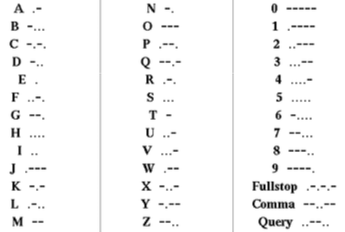
\includegraphics[scale=0.5]{apendice/problemas/problema1a/fig2.png}
\caption{Alfabeto \textit{Morse}}
\label{fig2}
\end{figure}

\subsection{Produto}
Um relatório no modelo de artigos da SBC com uma discussão detalhada sobre as três perguntas levantadas
e sobre a criptografia simplificada.
\subsection{Cronograma}

1 sessão tutorial e 1 aula expositiva.

\subsection{Recursos para aprendizagem}

\noindent
RAMOS, M. V. M.; JOSÉ NETO, J.; VEGA, I. S. \textbf{Linguagens Formais: Teoria, Modelagem e Implementação}. Editora Bookman, 2009.\\

\noindent
MENEZES, Paulo Blauth. \textbf{Linguagens formais e autômatos}. 6. ed. Bookman, 2011.\\

\subsection*{Referências}

Este problema é baseado no texto da Wilhelmiina Hamalainen\footnote{\url{https://www.researchgate.net/profile/Wilhelmiina_Haemaelaeinen}}.

\newpage
\section{\ProblemaH}
\subsection{Problema}
Os alunos da disciplina de Introdução as Linguagens Formais e Teoria da Computação normalmente
utilizam os computadores disponíveis em um dos laboratórios de informática da UFBA para
realização das atividades da disciplina.

Acontece que em um dia, os computadores de um destes laboratórios
de informática da UFBA começaram a apresentar um comportamento inesperado.

A primeira pessoa a relatar esse problema foi a Drissa.
Ela sentou de frente ao computador, como normalmente faz, mas ao digitar o próprio nome notou
que na tela estava escrito Qaxllo.
Ela tomou um susto sem entender o que estava acontecendo, então, como é amiga do Lucas, resolveu falar
com ele.
O Lucas estava sentado no computador ao lado, então ele tentou digitar Drissa no computador
que estava e percebeu que na tela apareceu Prsaaq.
O Lucas também tentou escrever o próprio nome e viu escrito na tela Dxwqa.

Então, Drissa e Lucas resolveram falar do problema para toda a turma, uma vez que não entenderam o
que estava acontecendo.
Em pouco tempo foi percebido que todos os computadores daquele laboratório estavam afetados
pelo problema.

A turma conversou rapidamente e percebeu que talvez este problema não seja muito difícil de resolver, então,
não precisariam esperar pelo atendimento do STI da UFBA, desta forma, resolveram fazer uma reunião para
discutir este problema e encontrar uma solução.

Quando todos já estavam saindo do laboratório para discutir o problema, o Angelmário, bastante atencioso,
alertou que não poderiam sair sem antes coletar mais informações para resolução do problema.
Então, assim foi feito, a Deuana e o Rodrigo foram os responsáveis por coletar o máximo de informações
possíveis.
Eles digitaram os nomes de todos os alunos da turma em cada um dos computadores e fizeram uma tabela de
correspondencia com o que era apresentado na tela.
Enquanto isso a Taiane disse que iria verificar se todos os cabos estavam
corretamente encaixados, ela constatou que todos os cabos estavam encaixados nos lugares certos.

\subsection{Produto}
Uma foto que demonstre que o problema está solucionado, bem como, um relatório que descreve os passos
para identificação e solução do problema, além de anexar todos os arquivos que julgar necessário.

\subsection{Cronograma}

1 sessão tutorial.

\subsection{Recursos para aprendizagem}
Não foram indicados recursos adicionais de aprendizagem.

\newpage
\section{\ProblemaI}
\subsection{Problema}
Os estudantes da disciplina de Introdução as Linguagens Formais e Teoria da Computação da UFBA
souberam na primeira aula da disciplina que será utilizada uma metodologia de ensino baseada
em problemas, então, eles resolveram pesquisar um pouco sobre a metodologia.

Os estudantes se reuniram para conversar sobre as coisas que tinham pesquisado.
Um dos estudantes disse que saber inferir informações implícitas em problemas é muito relevante
para que consigam obter bons resultados.
Outro estudante resolveu contar uma história e os demais ficaram atentos nos mínimos detalhes.

O estudante que conta a história diz que tudo começou na festa de aniversário da Alice.
Não, não a Alice do País das Maravilhas, mas uma amiga dele chamada de Alice:\\

--- Que tal preparar-nos umas tortas saborosas?---perguntou o Rei de Copas à Rainha de Copas num dia fresco de verão.

--- Fazer as tortas sem pimenta?---perguntou a Rainha.

--- Pimenta!---exclamou o Rei, incrédulo---Quer dizer que você usa pimenta em suas tortas?

--- Não muita---respondeu a Rainha.

--- E suponho que ela tem sido roubada!

--- É claro!---disse a Rainha---Encontre a pimenta e, quando descobrir quem a roubou, corte-lhe...

--- Vamos, vamos!---disse o Rei.

--- Bem, a pimenta tinha que ser encontrada, é claro. Agora, como todos vocês sabem, as pessoas que roubam pimenta nunca dizem a verdade.

--- O quê?!---disse Alice (não a Alice do País das Maravilhas, mas a Alice dessa festa)---Nunca ouvi falar disso antes!

--- Não ouviu?---perguntei-lhe, com falsa surpresa.

--- É claro que não! E tem mais, não acredito que ninguém mais tenha ouvido! Algum de vocês ouviu falar disso antes?

Todas as crianças abanaram a cabeça negativamente.

--- Bem,---disse eu---para fins desta história, vamos presumir que as pessoas que roubam pimenta nunca dizem a verdade.

--- Está bem---disse Alice, meio relutante.

--- Então, continuando a história, o suspeito mais óbvio era a cozinheira da Duquesa.

No julgamento, ela fez apenas uma declaração:

--- Eu sei quem roubou a pimenta!

--- Supondo que as pessoas que roubam a pi\-men\-ta sempre mentem, a cozinheira é culpada ou inocente?\\

PORTANTO, QUEM ROUBOU A PIMENTA?\\

Bem, os suspeitos seguintes do Rei foram a Lebre de Março, o Chapeleiro Louco e o Leirão. Os soldados foram mandados às casas deles, mas nenhuma pimenta foi encontrada. Mesmo assim, eles poderiam estar escondendo-a em algum lugar, de modo que foram detidos, com base nos princípios gerais.

No julgamento, a Lebre de Março afirmou que o Chapeleiro era inocente e o Chapeleiro afirmou que o Leirão era inocente. O Leirão resmungou uma declaração qualquer enquanto dormia, mas ela não foi registrada.

Como se constatou, nenhum inocente fizera uma afirmação falsa, e (como estamos lembrados) as pessoas que roubam pimenta nunca fazem afirmações verdadeiras. Além disso, a pimenta foi roubada por apenas uma criatura. Qual dos três é o culpado, se é que foi um deles?\\

ENTÃO, QUEM ROUBOU A PIMENTA?\\

--- Ora, ora, esse é realmente um caso difícil---disse o Rei.

Os suspeitos seguintes, curiosamente, foram o Grifo, a Falsa Tartaruga e a Lagosta.

No julgamento, o Grifo afirmou que a Falsa Tartaruga era inocente, e a Falsa Tartaruga disse que a Lagosta era culpada.
Mais uma vez, nenhum inocente mentiu e nenhum culpado disse a verdade.

Quem roubou a pimenta?

\subsection{Produto}
Um relatório no modelo de artigos da SBC para discutir se a cozinheira da história é culpada ou
inocente, se a Lebre de Março, o Chapeleiro Louco, o Leirão, o Grifo, a Falsa Tartaruga ou Lagosta
roubaram a pimenta.
É necessário detalhar cada inferência utilizada, por exemplo, ao inocentar ou acusar alguém, mostrar
quais as inferências e fatos utilizados para tal conclusão.

\subsection{Cronograma}
1 sessão tutorial.

\subsection{Recursos para aprendizagem}
Não foram indicados recursos adicionais de aprendizagem.

\section*{Referências}
Este problema é baseado no texto do Raymond Smullyan extraído do livro ``Alice no País dos Enigmas''.


\newcommand{\discursivaA}{%
\item{\textit{\textbf{Espaço para exposição livre sobre o problema:}}}}

\newcommand{\discursivaB}{%
\item{\textit{\textbf{Espaço para exposição livre sobre percepção do método PBL:}}}}

\newcommand{\discursivaC}{%
\item{\textit{\textbf{Espaço para exposição livre sobre a disciplina:}}}}

\newcommand{\discursivaProblema}[4]{%
\item{\textbf{Problema #1 - #2}}
\begin{itemize}
		{
		\discursivaA
		\begin{enumerate}
			#3
		\end{enumerate}
		}
		{
		\discursivaB
		\begin{enumerate}
			#4
		\end{enumerate}
		}
\end{itemize}}

\newcommand{\discursivaProblemaA}[3]{%
\item{\textbf{Problema #1 - #2}}
\begin{itemize}
		{
		\discursivaA
		\begin{enumerate}
			#3
		\end{enumerate}
		}
\end{itemize}}

\newcommand{\discursivaDisciplina}[3]{%
\item{\textbf{Estudantes #1}}
\begin{itemize}
		{
		\discursivaB
		\begin{enumerate}
			#2
		\end{enumerate}
		}
		{
		\discursivaC
		\begin{enumerate}
			#3
		\end{enumerate}
		}
\end{itemize}}

\xchapter{Respostas discursivas}{}
\acresetall
\label{apendice-qualitativo}

\begin{itemize}
\item{Semestre 2016.1}
	\begin{itemize}
	\discursivaProblema{1}{\ProblemaA}%
	{
	\item{O problema escolhido é muito complexo para
	uma tarefa inicial do curso e que tem dependencia real com a musica.}
	\item{Talvez, por ser o primeiro problema, o desempenho na
	maioria dos grupos foi regular.}
	}%
	{
	\item{Fazer um trabalho com uma equipe ruim foi a para mais complicada.}
	\item{A metodologia é interessante porém, como estamos tentando
	fazer, necessita de aprimoramentos. A alternância entre aula teórica
	e sessões tutorial me pareceu mais eficaz do que somente sessões
	tutorial.
	No mais a metodologia parece ser bem promissora se bem trabalhada.}
	\item{Gostei do método de ensino.
	Já sabia como funcionava, mas foi minha primeira participação em um.
	As reuniões foram bem úteis e o ambiente foi muito colaborativo.}
	\item{O PBL é muito interessante, pois, estimula o trabalho
	colaborativo que por consequência leva a soluções mais rápidas.}
	}
	
	\discursivaProblema{2}{\ProblemaB}%
	{
	\item{O problema deve ter mais regras como preços da
	maquina ou valores aceitos para amarrar o problema ao conteúdo.}
	\item{Achei que a descrição do problema não ficou claro,
	um exemplo bem claro é que fala somente sobre o troco aleatório
	e não sobre o troco quando a entrada é acima do valor do produto.}
	}%
	{
	\item{o método está de acordo, mas o \textit{feedback} dos trabalhos está insuficiente.}
	\item{Essa segunda atividade foi melhor que a primeira, acho que a
	turma está conseguindo entender e discutir melhor.}
	}

	\discursivaProblema{3}{\ProblemaC}%
	{
	\item{o tempo e dificuldade estavam bem equilibrado.
	Poderia se dificultar um pouco se houvesse mais tempo ou uma equipe. Se a proporção fosse independente do carro.}
	}
	{
	\item{Os alunos têm participado mais das aulas.}
	}

	\discursivaProblemaA{4}{\ProblemaD}%
	{
	\item{O problema foi útil para aprendizagem, no entanto é
	necessário realizar a construção de outras máquinas antes
	de pedir uma de forma avaliativa.
	A máquina do problema não era difícil, porém, antes de
	fazer uma máquina que abrange tantas possibilidades,
	seria mais produtivo construir algumas mais simples em
	sala, para que todos tivessem a oportunidade de adquirir
	o conhecimento mais básico, além da teoria passada nas
	aulas expositivas.}
	}

	\discursivaProblema{5}{\ProblemaE}%
	{
	\item{O problema da parada é muito complicado para um
	período de tempo curto, além de ter poucos encontros.
	Em vez de fazer encontros para cada problema e fixar
	na resolução individual e com encontros programados,
	poderia fazer uma apresentação de alguns problemas
	maiores e ao longo do semestre encontros mais
	distantes para a resolução do problema.}
	}
	{
	\item{O PBL é muito bom quando bem aplicado.
	Acho que a quantidade de problemas poderia ser menor
	e a dificuldade dos problemas poderiam ser maiores,
	ex: passaria um problema de autômato finito até autômato
	com pilha, com mais encontros, ou até maquina de turing...
	Para que assim a resolução do problema envolva diversos
	assuntos, e que depois venha o conteúdo fazendo o
	fechamento do método PBL.
	E a mesma coisa poderia ser utilizada para os
	outros assuntos.}
	}

	\discursivaDisciplina{concluintes}%
	{
	\item{Acho que seria muito útil a criação de máquinas em sala,
	não apenas sua exposição e explicação de como funciona.}
	\item{O método PBL reque mais esforço do aluno e um trabalho
	em conjunto de todos os participantes.
	O ideal para usar o método PBL é que os participantes estejam
	motivados para resolver o problema e achar este motivador é
	o que pode fazer a diferença.}
	}
	{
	\item{Acho que mais aulas expositivas seria uma boa ideia.
	Foram muitas atividades avaliativas, concordo em número de
	atividades, mas não que todas sejam pontuadas.
	Para última prova, como disse em sala, aconselho que seja
	menos conteúdo ou que tenha um peso maior.}
	\item{A disciplina foi ótima.}
	}
	
	\discursivaDisciplina{desistentes}%
	{
	\item{Achei interessante o PBL, mas achei que deveria ter
	sempre antes de expor um problema, fornecer uma base/start
	para que o estudante não perca muito tempo buscando algo sem
	sentido à ser aplicado ao problema e nos debates em sala,
	pois facilmente acaba fugindo do assunto, com isso a expansão
	do cenário.
	Sobre este último ponto, estas atividades de resolução de
	problemas, costumam demandar um longo periodo de análise.
	Sei sobre isto na prática, porque 2h ou 3h para mim não é
	nada quando se trata de problemas para se resolver.
	Como muitos estudantes possuem outras matérias na maioria
	das vezes, meio que é preciso ter algum resultado no tempo
	restrito de estudo, isto principalmente para quem trabalha,
	que é no caso do turno noturno.}
	}%
	{
	\item{Gosto da disciplina, mas acho que um caso geral que é
	normal de acontecer é de não saber o perfil da turma no momento
	de aplicar uma metodologia, as cobranças dia/aula foi o mais
	complicado mesmo, pois era algo que demandava de você ter sempre
	algo produzido, o que poucas vezes acontecia, porque como eu
	citei no quadro anterior, as 3h de dedicação da disciplina não
	adiantava, porque eu não conseguia fazer uma abordagem precisa,
	ficando bastante perdido, ainda mais com mais disciplinas.
	A questão não é dizer que uma disciplina é mais importante que
	a outra em termo de aprendizado, mas o curso atual de sistemas
	de informação, obriga você a priorizar as disciplinas,
	infelizmente, devido ao fluxograma e suas matérias
	pré-requisitos.
	Por fim, existe um contexto a cada nova turma.
	Acho que uma pesquisa inicial de perfil de turma, no inicio
	da disciplina, ajude a melhor conciliar a metodologia, mesmo
	a UFBA demonstrando o que muitos estudantes acham que
	``ela não está ligando para quem trabalha''.}
	}
	\end{itemize}

\item{Semestre 2017.1}
	\begin{itemize}
	\discursivaProblema{1}{\ProblemaG}%
	{
	\item{Achei esse problema muito extenso, gostaria de um
	\textit{feedback} para saber se realmente fiz corretamente,
	ainda mais que foi individual, não sei se conseguir
	entender realmente.}
	\item{O problema trazia pessoas que tinham acabado de
	ser resgatadas de um acidente, mas ao invés de passar
	mensagem às suas famílias, o que seria o mais lógico
	racional e irracionalmente, eles focam em enviar mensagem
	criptografada pro trabalho de um sistema criado.}
	}
	{
	\item{É interessante que as equipes sejam formadas e
	mantidas ao longo da disciplina e que recomendem esse
	grupo fixo e que alguém pegue telefone nome e email de
	todos, para facilitar posteriormente.}
	\item{Houve bastante dificuldade de entendimento
	do que era requerido.
	O problema deixou as possibilidades de resposta tão
	abertas que o grupo se perdeu.
	Nenhuma outra disciplina utiliza esse método,
	então é necessária uma maior atenção aos alunos na
	interpretação do que se requer.}
	}

        \discursivaProblema{2}{\ProblemaB}%
	{
	\item{Não ficou claro para mim o objetivo em relação
	com o escopo da disciplina}
	\item{Creio que apenas este problema em si não despertou
	a motivação necessária e tempo hábil, levando em consideração
	a exigência de outras matérias e período de primeiras
	avaliações para a conclusão de um bom trabalho.
	A construção da máquina de estados é maravilhosa,
	mas ainda um pouco confusa quando requer uma grande
	quantidade de estados.}
	\item{Tive mais facilidade com esse do que o anterior}
	\item{Foi bastante chocante a diferença de nível pro problema anterior.
	Isso dificultou o aprendizado.}
	\item{O problema foi bom, só que em alguns momentos as
	sessões se tornam cansativas e as pessoas ficam dispersas.}
	\item{Talvez a forma com que o problema que iremos submeter,
	seja a deficiência do método de aprendizado.
	Nem todos grupos chegam a uma solução que seja clara para
	todos os componentes.
	Existem componentes muito mais avançados do que outros na
	questão do desenvolvimento da solução e essa diferença não
	deixa claro o ``produto bruto'' das reuniões.
	As respostas do grupo não ficam claras de forma geral.}
	}
	{
	\item{É um método muito bom para atividades e desenvolvimento em grupo.
	Para submeter atividades individuais só favorece aqueles que tem
	conhecimento mais avançado e conseguem sozinhos resolver o problema
	desde o inicio, pois das reuniões alguns alunos não extraem
	as informações, tornando as reuniões de certa forma, indiferentes.}
	\item{O método é enriquecedor sem o processo massante de alguns
	aprendizados, a aula me desperta e faz ter \textit{insights} para a
	resolução de alguns problemas que antes não conseguiria identificar.}
	\item{Ficamos um pouco perdidos sobre o que fazer,
	o que era/como fazer autômato.
	Faltou uma aula teórica mais demonstrativa antes, de como fazer
	funcionar um autômato.}
	\item{Acredito que o quadro não fique responsável apenas
	para uma pessoa, faz com que as outras não se sintam
	intrusas do grupo e queiram participar de fato.}
	\item{Outro ponto importante é que as vezes não existe a
	cooperação por parte dos colegas em relação as
	funções (mesa, quadro...), sendo assim muitas vezes uma pessoa
	repete a função várias vezes e outros pegam o ``bonde'',
	e não se comprometem com a disciplina, dizendo que é por
	causa do trabalho, família, enfim de modo geral não
	se compromete com a matéria e com a equipe que ele
	faz parte. }
	}
        \discursivaProblema{3}{\ProblemaC}%
	{
	\item{A grande dificuldade talvez esteja em já pensar
	em soluções sem ter o mínimo de conhecimento sobre como resolver.
	Isso dificulta a ação de similar o que o problema quer passar,
	só sendo possível nas últimas aulas, quando o limite de tempo
	já está prestes a estourar.}
	\item{Achei que o problema teve uma dificuldade média de solução,
	mas foi de difícil interpretação.
	O texto continha muitas metáforas desnecessárias
	(balança, via secundária para desvio) que desviavam
	a atenção do problema principal e atrapalhavam sua solução.
	A dificuldade média se deve a não ter sido fácil para a
	maioria entender como as proporções 3:5 e 2:5 seriam atendidas,
	mas depois que o segredo foi desvendado,
	vimos que o autômato era bastante simples.}
	\item{Foi o problema mais complicado, mas também o que se aprende mais.}
	}
	{
	\item{OK.}
	\item{Funcionou muito bem para o meu aprendizado,
	pois senti mais vontade de participar das aulas e me senti
	em muitos momentos desafiado a expor claramente meu pensamento, 
	a escutar com paciência a ideia do outro e a solucionar o problema.
	Porém, não vi o mesmo acontecer com outras pessoas.
	Algumas delas tinham sempre uma postura passiva ou
	desinteressada, o que em alguns momentos era
	frustrante, mesmo para mim.
	Fico a refletir se isso aconteceria por esse não ser
	o melhor método de aprendizagem para essa pessoas,
	ou por razões pessoais como falta de motivação ou
	interesse com o curso ou disciplina.
	Talvez a metodologia tenha até ajudado essas pessoas
	de alguma forma, mas quanto a isso não posso afirmar.}
	}
        \discursivaProblema{4}{\ProblemaD}%
	{
	\item{É um problema real, então foi interessante lidar com ele.}
	\item{Nesse problema específico, tive dificuldades em conseguir
	entender o que era pedido, visto que não tinha nenhum conhecimento
	prévio sobre MT, o que criou uma barreira para o aprendizado,
	ao invés de incentivar a aprendizagem.}
	\item{Não sobre o problema, mas sobre a formação da equipe.
	Teoricamente teriam as mesmas pessoas, portanto, mesma quantidade
	de membros na equipe.
	Mas não sei se foi impressão minha mas aparentava ter menos pessoas
	nas sessões tutoriais.
	Nesse problema minha equipe teve um desempenho melhor no
	entendimento e resolução do problema.
	Acredito que o fato de ter menos gente influenciou em
	as discussões acontecerem de forma mais otimizada,
	já que todos participavam.}
	}
	{
	\item{É bom para aprender entre colegas.}
	}

        \discursivaProblema{5}{\ProblemaE}%
	{
	\item{Difícil, mas interessante.}
	}
	{
	\item{Como nunca havia participado desse método,
	sinto que fiquei pra trás por não acompanhar os
	estudos atentamente desde o início.}
	}
        
	\discursivaProblema{6}{\ProblemaF}%
	{
	\item{N=NP? Pergunta de 1 milhão de dólares.
	Quando resolvida irá solucionar o problema do
	caixeiro viajante.
	Como o assunto é puramente matemático não invocou
	muita vontade de resolver.}
	\item{Tive um pouco de dificuldade para entender.}
	}
	{
	\item{Não me adaptei ao método.}
	\item{Não consegui chegar a uma reposta que eu tivesse certeza,
	mesmo olhando todos os materiais disponíveis e extras,
	o método PBL traz isso de procurarmos as respostas,
	mas se eu não consigo encontrar acaba me desmotivandoe
	nas sessões tutoriais mesmo com dicas,
	eu me sinto um pouco perdida no conteúdo.}
	}

	\discursivaDisciplina{concluintes}%
	{
	\item{Eu não me adequei ao método.
	Não consegui absorvê-lo.
	Por isso perdi na disciplina. :(
	É um método interessante e inteligente, mas não é para mim.}
	\item{Foi interessante e desafiador ter contato com um
	método tão diferente do usual.
	A maioria das sessões teve como efeito me motivar para
	solucionar os problemas e assim aprender mais profundamente
	o conteúdo da disciplina, porém, tal efeito não durou
	até o final do semestre, e com certeza não se estendeu
	a todos os estudantes matriculadas na disciplina.
	Nas rodas de discussão sempre houveram alguns alunos
	desinteressados e a cada aula o número de desinteressados
	aumentava, o que tornava difícil proegredir com as discussões.
	Além disso, o cansaço causado pela faculdade e o
	aumento da complexidade e dificuldade dos desafios
	contribuiram para que as sessões perdessem
	sua produtividade.}
	\item{A metodologia é perfeita pra aprendizagem na matéria.}
	}
	{
	\item{Disciplina que não entendi muito bem.
	As aulas práticas me deram uma luz, sem elas,
	minhas notas seriam mais baixas do que foram.
	Consegui aprender apenas quando estava no grupo.}
	\item{A pessoa fica meio perdida se faltar alguma
	aula de sessão tutorial, comprometendo as outras.
	Percebi colegas se atrapalhando muito
	ao fim da matéria.
	A presença se torna algo muito importante mais do
	que nos outros cursos pois se a pessoa faltar num
	dia perderia o assunto e no outro perderia a atividade.
	Talvez o assunto devesse ser revisado no dia da
	atividade em grupo.}
	\item{Foco na parte final do conteúdo, uma vez que
	é do de mais difícil compreensão}
	}

	\end{itemize}

\end{itemize}

% \include{apendice2}
% ...
% \include{apendiceM}

%% Fim do documento
\end{document}
%------------------------------------------------------------------------------------------%
